\documentclass[11pt]{book}
\usepackage{amsmath,amssymb,amsfonts}
\usepackage[spanish]{babel}
\usepackage{iiit_thesis}
\usepackage{cite}
\usepackage{times}
\usepackage{graphicx}
\usepackage{setspace}
\usepackage{enumitem}
\usepackage{tabularx}
\usepackage{subfig}
\usepackage{notoccite}
\usepackage{afterpage}
\usepackage{xcolor}
\usepackage{algorithm}
\usepackage{algpseudocode}
\usepackage{multirow}
\usepackage[hidelinks]{hyperref} 
\usepackage[toc,page]{appendix}
\usepackage{comment}
\usepackage{pdfpages}
\usepackage{siunitx}
%\usepackage{subcaption}
\usepackage{float}
\usepackage{MnSymbol}
\usepackage[labelfont=bf]{caption}
\captionsetup{labelfont=bf}

%\usepackage[table,xcdraw]{xcolor}


\newcommand{\img}[4]{\begin{figure}[H]\centering \includegraphics[width=#2\textwidth]{#1} \caption{#3} \label{#4} \end{figure}}

%roman sections
%\renewcommand{\thechapter}{\Roman{chapter}}
%\renewcommand\thesection{\thechapter.\Roman{section}}
\renewcommand\thesubsection{\Alph{subsection}}

%fontsize of chapter
\usepackage{titlesec}    
\titleformat{\chapter}[display]
{\normalfont%
    \centering\LARGE% %change this size to your needs for the first line
    \bfseries}{\centering\chaptertitlename\ \thechapter}{20pt}{%
    \huge %change this size to your needs for the second line
    }
    
%header

\newcounter{anexo}[section]
\newenvironment{anexo}{\refstepcounter{anexo}\par\medskip\noindent
   \textbf{ANEXO~\theanexo.} \rmfamily}{\medskip}
 \renewcommand{\theanexo}{\Alph{anexo}}
\newcounter{apendice}[section]
\newenvironment{apendice}{\refstepcounter{apendice}\par\medskip\noindent
   \textbf{APÉNDICE~\theapendice.} \rmfamily}{\medskip}
 \renewcommand{\theapendice}{\Alph{apendice}}



\graphicspath{{images/}{./}} % To include images in other directories

%------------------------------------------------
% To reduce separation in itemize and enumerate
% \setlist[itemize]{noitemsep} % can include 'nolistsep' also
% \setlist[enumerate]{noitemsep}

%------------------------------------------------
% Settings for Abbreviations and Symbols list
\usepackage[style=super,automake,nogroupskip,nopostdot,symbols,sort=standard,toc=false]{glossaries-extra}
\setglossarystyle{super}
\setabbreviationstyle[acronym]{long-short}
  % \centering
  \renewenvironment{theglossary}%
    {\tablehead{}\tabletail{}%
     \begin{supertabular}{p{4cm}p{\glsdescwidth}}}%
    {\end{supertabular}}%
\makeglossaries
\loadglsentries{acronyms}

%-------------------------------------------------
\long\def\symbolfootnote[#1]#2{\begingroup%
\def\thefootnote{\fnsymbol{footnote}}\footnote[#1]{#2}\endgroup}
\renewcommand{\baselinestretch}{1.2}
\onecolumn
%
\makeatletter
\def\ignorecitefornumbering#1{%
     \begingroup
         \@fileswfalse
         #1%                     % do \cite comand
    \endgroup
}
\makeatother

%-------------------------------------------------
% Custom commands
\newcommand{\p}{\mathbb{P}}
\newcommand{\gt}{\gamma_{\text{th}}}
\newcommand\txtblue[1]{{\color{blue}#1}}
%--------------------------------------------------------





\begin{document}
\renewcommand{\tablename}{Tabla}
\pagenumbering{roman}
%% TITLE PAGE
\thispagestyle{empty}
\begin{center}

%\vspace*{2cm}
{
\includegraphics[width=5cm]{figures/UBA_logo.png}\\}
\vspace*{2mm}
{\large Universidad de Buenos Aires\\}
{\large Facultad de Ciencias Exactas y Naturales\\}
{\large Departamento de Física\\}
%\vspace*{5mm}
%{ Intendente Güiraldes 2160, Buenos Aires, Argentina\\}
%\vspace*{5mm}


\vspace*{2cm}
{\huge \bf Transformación de la memoria autobiográfica: análisis de cambios en el discurso}

%\bf
% \vspace*{2.2cm}
% {\large A thesis submitted in partial fulfillment\\}
% {\large  of the requirements for the degree of \\}

\vspace*{1cm}
{\it {\large Tesis de Licenciatura  en Física} 
}

\vspace*{0.8cm}


\vspace*{6mm}
{\Large Corina Révora\\}
%{\large LU: 283/18\\
%{\small \tt cori.revora@gmail.com}}

\vspace*{10mm}
{\large Dirección: Luz Bavassi\\}
{\large Co-Dirección: Lauta Kaczer\\}


\vspace*{5mm}
{\large Marzo 2024\\}
\end{center}

\newpage

{\large TEMA:  Transformación de la memoria autobiográfica: análisis de cambios en el discurso}\newline
%\vspace*{0.01cm}\newline

{\large ALUMNA: Corina Révora}\newline
%\vspace*{0.02cm}\newline

{\large LU: 283/18}\newline
%\vspace*{0.02cm}\newline

{\large LUGAR DE TRABAJO: Laboratorio de Neurociencias de la Memoria (IFIByNE, UBA-CONICET). }\newline
%\vspace*{0.02cm}\newline

{\large DIRECCIÓN: Luz Bavassi (UBA/CONICET y algo mas?) y Laura Kaczer (UBA/CONICET algo mas?)}\newline

%\vspace*{0.02cm}\newline
{\large FECHA DE INICIACIÓN: Marzo 2023}\newline
%\vspace*{0.02cm}\newline

{\large FECHA DE FINALIZACIÓN: Marzo 2024}\newline
%\vspace*{0.02cm}\newline

{\large FECHA DE EXAMEN: algundia/03/2024 }\newline
%\vspace*{0.02cm}\newline

{\large INFORME APROBADO POR: }

\vspace*{1.5cm}
\begin{center}
    \renewcommand{\arraystretch}{4.5} % Ajusta la altura de las filas
    \large % Tamaño de fuente más grande para el contenido de la tabla
    \begin{tabular}{|p{7cm}|p{7cm}|}
        \hline
        \multirow{1}{7cm}[2em]{ Autor} & \multirow{1}{5cm}[2em]{ Jurado} \\
        \hline
         \multirow{1}{7cm}[2em]{ Director} & \multirow{1}{5cm}[2em]{ Jurado} \\
        \hline
        \multirow{1}{7cm}[2em]{ Profesor de la Tesis de Licenciatura} & \multirow{1}{5cm}[2em]{ Jurado}\\
        \hline
    \end{tabular}
\end{center}




%------------------------------------------------
%\newpage
\thispagestyle{empty}
\vspace*{1.5cm}
\begin{center}
{\Large International Institute of Information Technology Hyderabad\\}
{\Large Hyderabad, India\\}
\vspace*{3cm}
{\Large \bf CERTIFICATE\\}
\vspace*{1cm}
\noindent
\end{center}
This is to certify that work presented in this thesis proposal titled \textit{\textbf{Title of the research thesis}} by \textit{Name of the author} has been carried out under my supervision and is not submitted elsewhere for a degree.

\vspace*{3cm}
\begin{tabular}{cc}
\underline{\makebox[1in]{}} & \hspace*{5cm} \underline{\makebox[2.5in]{}} \\
Date & \hspace*{5cm} Advisor: Dr. Firstname Lastname
\end{tabular}
\mastersthesis
% \renewcommand{\baselinestretch}{1.5}
%
% ABSTRACT PAGE
%\chapter*{Resumen}
%\label{ch:abstract}
%% \begin{itemize}
%     \item 
%     \item  
%     \item 
%     \item 
%     \item 
% \end{itemize}

\textbf{Palabras Clave:} Memoria Autobiográfica, Procesamiento de Lenguaje Natural, Entrevista Autobiográfica, Evaluación Automatizada, Aprendizaje No Supervisado
%
\tableofcontents
%\listoffigures
%\let\cleardoublepage\clearpage
%\listoftables
%\printglossary[type=\acronymtype,title=Abbreviations,nonumberlist]
%\printunsrtglossary[type=symbols]

%--------------------------------------------------------
% 'List of Publications'
%\chapter*{Lista de Publicaciones Relacionadas}
%\label{ch:relatedPubs}
%\begin{enumerate}[label={[P\arabic*]}]  
    \item Author1, Author2, and Author3, \textbf{``Title of the paper published in the conference or journal"}, in proceedings of {\it IEEE International Symposium on the name of the conference or journal}, 2020.
    
    \item Author1, Author2, and Author3, \textbf{``Title of the paper published in the conference or journal"}, in proceedings of {\it IEEE International Symposium on the name of the conference or journal}, 2020.

    \item Author1, Author2, and Author3, \textbf{``Title of the paper published in the conference or journal"}, in proceedings of {\it IEEE International Symposium on the name of the conference or journal}, 2020.
    
\end{enumerate}
\noindent
Related co-author publications:
\begin{enumerate}[start=3,label={[P\arabic*]}]
    \item Author1, Author2, and Author3, \textbf{``Title of the paper published in the conference or journal"}, in proceedings of {\it IEEE International Symposium on the name of the conference or journal}, 2020.
    
    \item Author1, Author2, and Author3, \textbf{``Title of the paper published in the conference or journal"}, in proceedings of {\it IEEE International Symposium on the name of the conference or journal}, 2020.

\end{enumerate}

%\chapter*{Agradecimientos}
%\begin{itemize}
    \item familia 
    \item la gente del labo
    \item a la facultad
    \item luz y lau
    \item compas de carrera y menciones: gabi por los labos? sony el puercoespin, carli y rosen, toddys
    \item gente que me haya tutelado: gabi capelutto 
\end{itemize}

%--------------------------------------------------------
%\chapter{Introducción}
%\label{ch:intro}
%
%----------------------------------------------
\section{:)))))}

Cosas sobre memorias autobiográficas, mira tesis de Juani y Constanza
Citar los papers de los que sacamos medidas al contar sobre estas medidas para justificar las herramientas que usamos para analizar
Al final escribir objetivos


%---------------------------------------------------------



%--------------------------------------------------------
\chapter{Materiales y métodos}
\label{ch:ch2}
\section{Participantes}\label{paracitar}
Acá tengo que contar la edad de los participantes, el género y esas cosas como estan en los papers
\section{Entrevista Autobiográfica}
aca tengo que contar el experimento que vinieron 65 personas a contar relatos libres de memorias autobiográficas sobre cuatro eventos del 2022 y un evento de control que era la memoria no consolidada. Cómo se seleccionaron los eventos? PONER LA ELECCIÓN DE LOS EVENTOS EN APÉNDICE: Los eventos se seleccionaron buscando los eventos mas relevantes del 2022 en diarios, tendencias de google y tendencias de tw. Se realizó una encuesta con los 30 eventos del 2022 a 100 personas contar estas 100 personas la edad y esas cosas. Mostrar gráfico de intensidad vs valencia de los eventos seleccionados, cuánto recordaron de cada uno en presencial solo de menores de 30. 
Del experimento tengo que contar que venian a hablar, antes se les hacia el cuestionario de Memorias autobográficas el día antes. El día de la entrevista al llegar se les mostraba una instrucción donde se les contaba de que constaba el experimetnto y se relataba que contaran de sobre sus vivencias propias el día que se enteraron del evento sobre el que se les iba a preguntar. Se arrancaba con un relato control para que entraran en calor, el relato no consolidado y dsp se preguntaba en orden aleatorio por los otros 4 eventos. Las ques se presentaban con diapositivas que pasaban ellos. Se grababa un audio de los relatos. Después de la entrevista se hacía las mismas preguntas que se hicieron para seleccionar los eventos: cuáto recordaron y la intensidad y valencia del sentimiento al recordar. Esto se repitió nuevamente 5 meses después a esta entrevista retornaron un x porciento de los participantes nuevamente demografía de los mismos.
Los relatos se grababan y transcribian usando whisper el paquete large, después pasaban por una corrección humana ya que whisper asegura un 98 porciento correcta al transcripción. Se corregía las palabras y la puntuación.
\section{Herramientas NPL}

Para analizar los relatos se introdujeron herramientas de NLP (tengo q hablar de NLP en la intro) buscando cuantificadores de los relatos que nos dejen estudiar los mismos separanado por bla y bla. Lo primero que se hizo fue descartar outliers contando la cantidad de palabras únicas en los relatos descartando a las personas a 3 MADs de distancias de la media (CITAR PAPER SUEÑOS DE ITBA DONDE HACEN ESTO), dejo cuántas personas tienen cada relato? No, mejor solo pongo el porcentaje que descarta esto. Las variables se separaron en 4 categorías, ponerlas con subindices y explicarlas. contenido sentimiento estructurales y memoria.
\section{Reducción de dimensionalidad y clustering}
aca contar de PCA (de TSNE no pero decir que se probaron otros algoritmos de reducción de dimensionalidad y se decidió por este). Contar de clustering, decir que se usaron otros métodos pero daban todos parecidos entre kmedoids kmeans y jerarquico con average y se decidió por kmeans porque era levemente mejor. Contar del índice R (ve performance con data externa), las matrices de confusión, silhouette (ve performance con respecto a lo interno).

Toca explicar el quilombo que hice para separar, que primero fue presencial vs filler, de silhouette se define k, de R el nro de PCs, y viendo las PCs se toman las variables mas significativas de estas PCs, explicar el criterio de cómo se eligen esas variables, y que se hace un barrido. Se tienen las PCs que maximizan esta separación. Se ve que pasa en el segundo con ESTAS PCs.
Después se busca separar cfk, ar y campeones, primero buscamos usando todas las vars nro pcs vs k silhouette y se definió k, dsp  n vs nro pcs una matriz del R pare definir n y nro PCs. Se tienen las PCs que maximizan la separación en el primer tiempo. Se ve que pasa en el segundo tiempo con ESTAS PCs.

Se pasa a comparar los dos tiempos las PCs que separaban cfk ar y camp se usan para comparar en el primer tiempo vs en el segundo usando ANOVA a ver si hay diferencias entre las medias. Se hizo condición a condición.

%--------------------------------------------------------
\chapter{Resultados}
\label{ch:ch3}
\section{Participantes}
las caracteristicas de los participantes en tablas demográficas o gráficos (?? no me cierra. También el resultado del cuestionario. También cuestioario preentrevista de ellos. Se podría hacer estadística de si cambió esto haciendo anova de medidas repetidas. Le tengo que pasar los datos a Lau. Aclarar que todavía de todos los participantes, después descarto los OUTLIERS y que no todos los participantes respondieron la posetentrevista, dar el porcentaje que lo hizo. De nuevo, sin poner filler.


\section{Variables de las herramientas de NPL}
 
 El segundo tiempo ver qué hago, puedo poner en apéndice o si veo que se ven parecidos decir que no tiene diferencias significativas el gráfico.

Se buscó los diferentes cuantificadores mencionados en la sección \colorbox{yellow}{CITAR} para los relatos de la primer y segunda entrevista por separado. A continuación se muestran los resultados de algunas de los cuantificadores obtenidos para la primer entrevista, los de la segunda entrevista \colorbox{yellow}{o se pueden buscar en el apéndice o que son resultados similares} \colorbox{yellow}{en metodos no me tengo que olvidar de mencionar que se descartan los outliers}

\begin{comment}
Esto está desactivado temporalmente.
\begin{figure}[H]
    \centering
    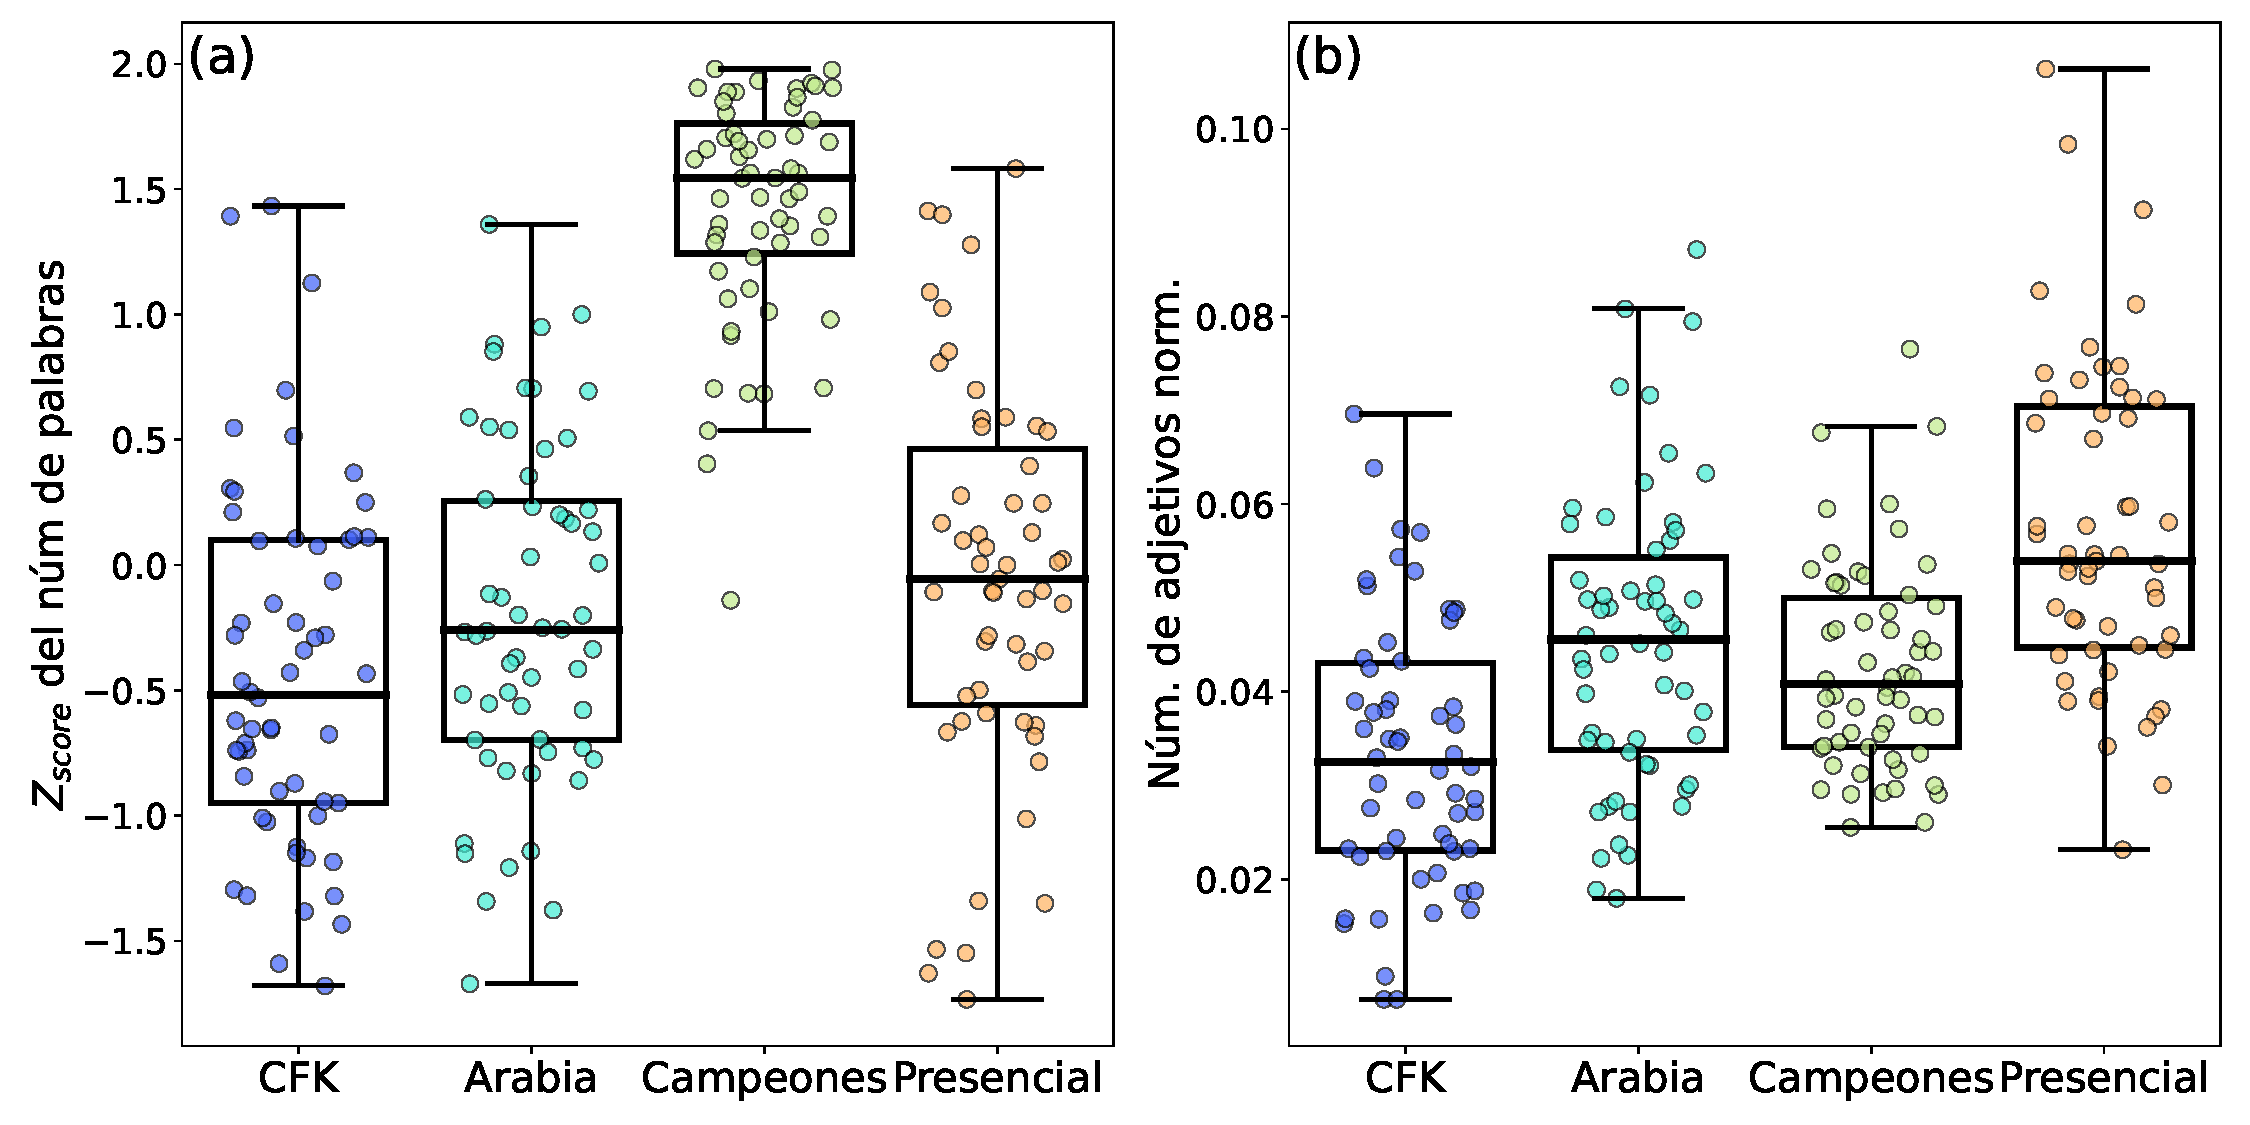
\includegraphics[width = 15cm]{figures/ch03/Herramientas NPL/Primer tiempo/Sin control/contenido_boxplot.pdf} 
    \caption{\textbf{(a)}  \textbf{(b)}}
\label{fig:cap3_vars_contenido}
\end{figure}

\begin{figure}[H]
    \centering
    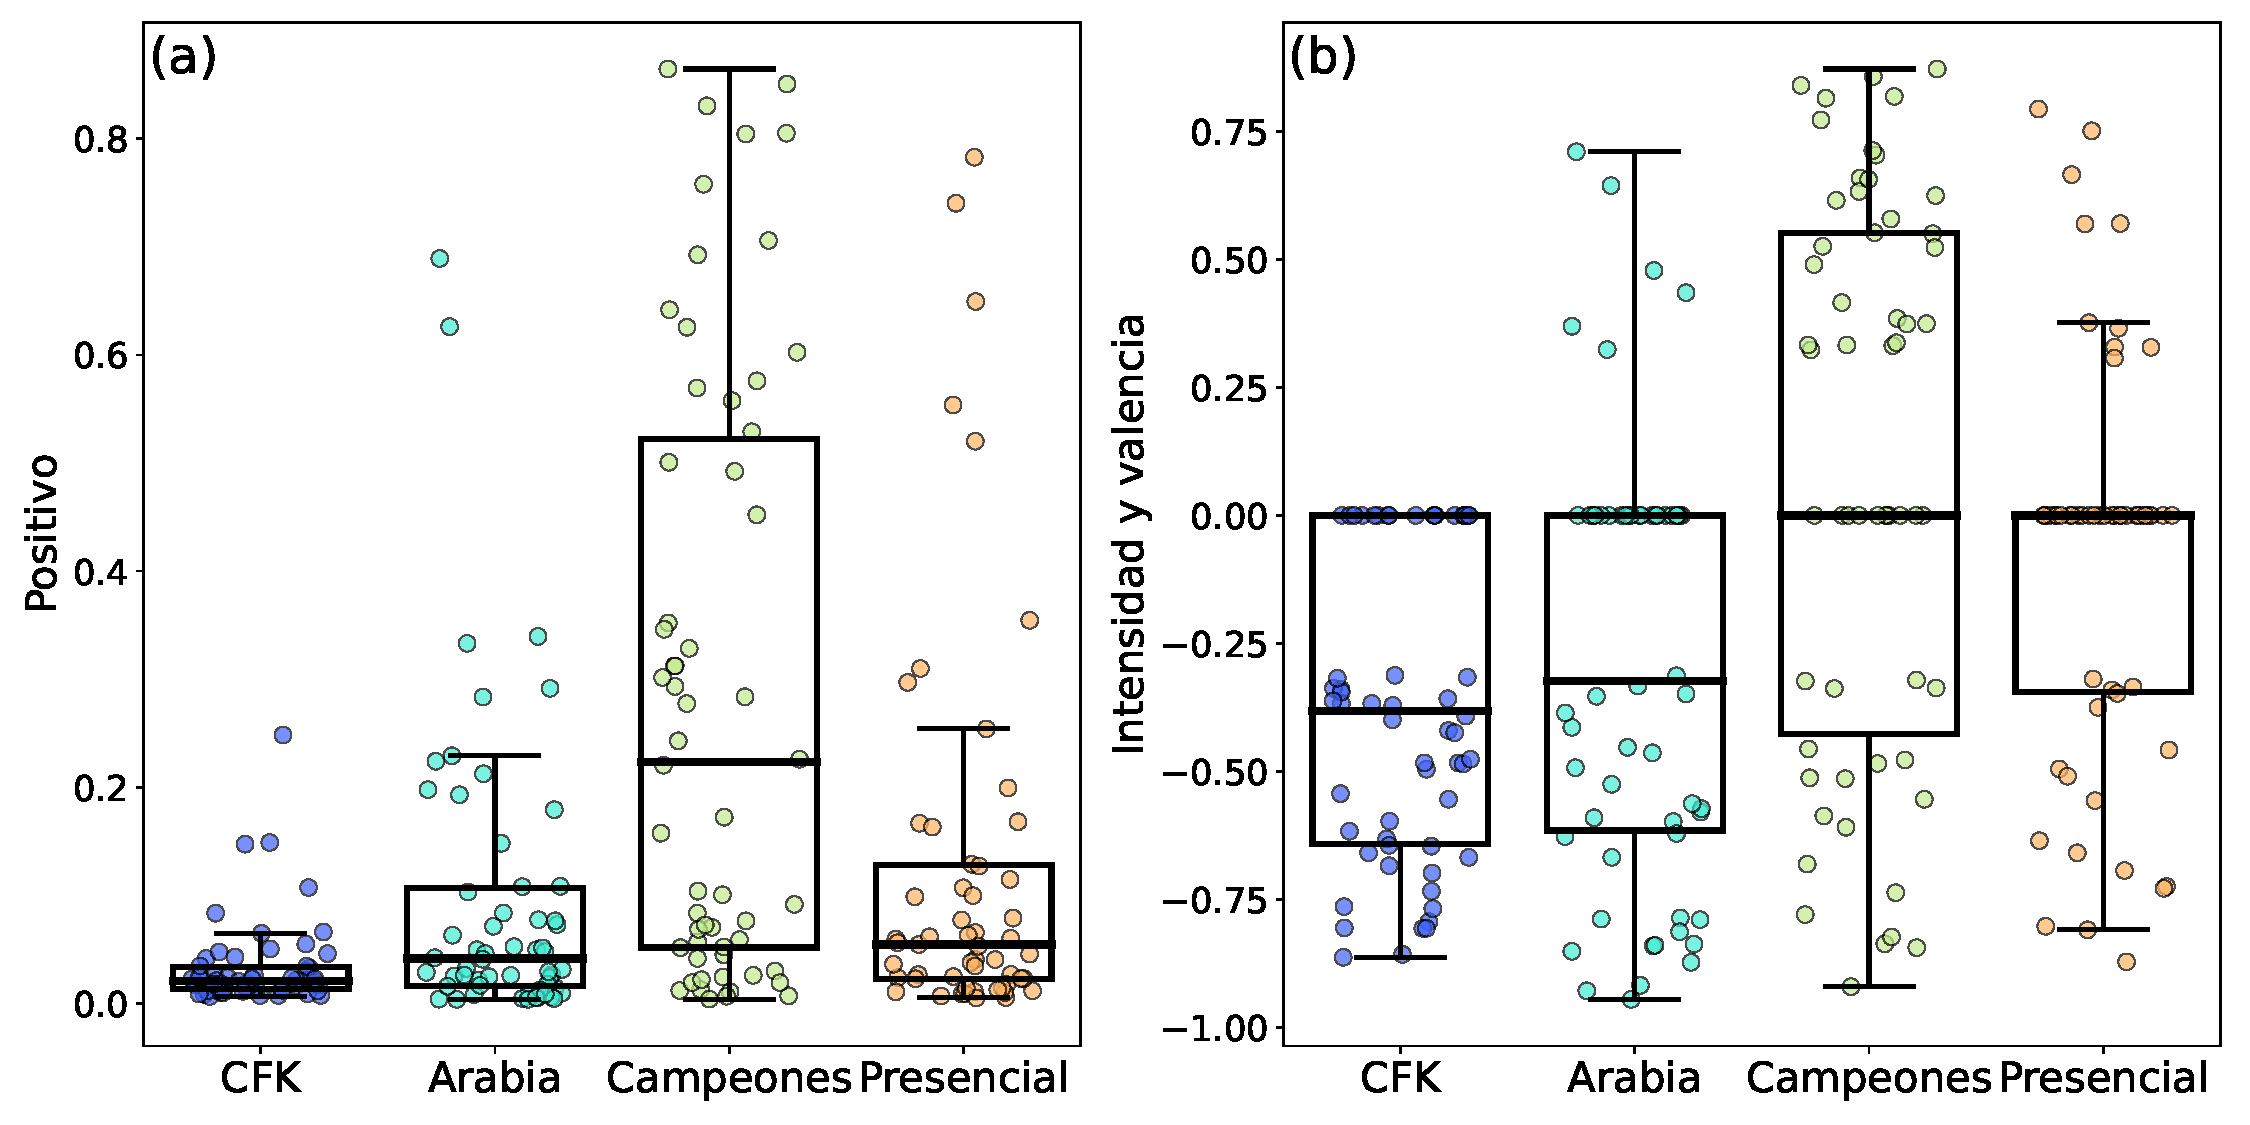
\includegraphics[width = 15cm]{figures/ch03/Herramientas NPL/Primer tiempo/Sin control/sentimiento_boxplot.pdf} 
    \caption{\textbf{(a)}  \textbf{(b)}}
\label{fig:cap3_vars_sentimiento}
\end{figure}

\begin{figure}[H]
    \centering
    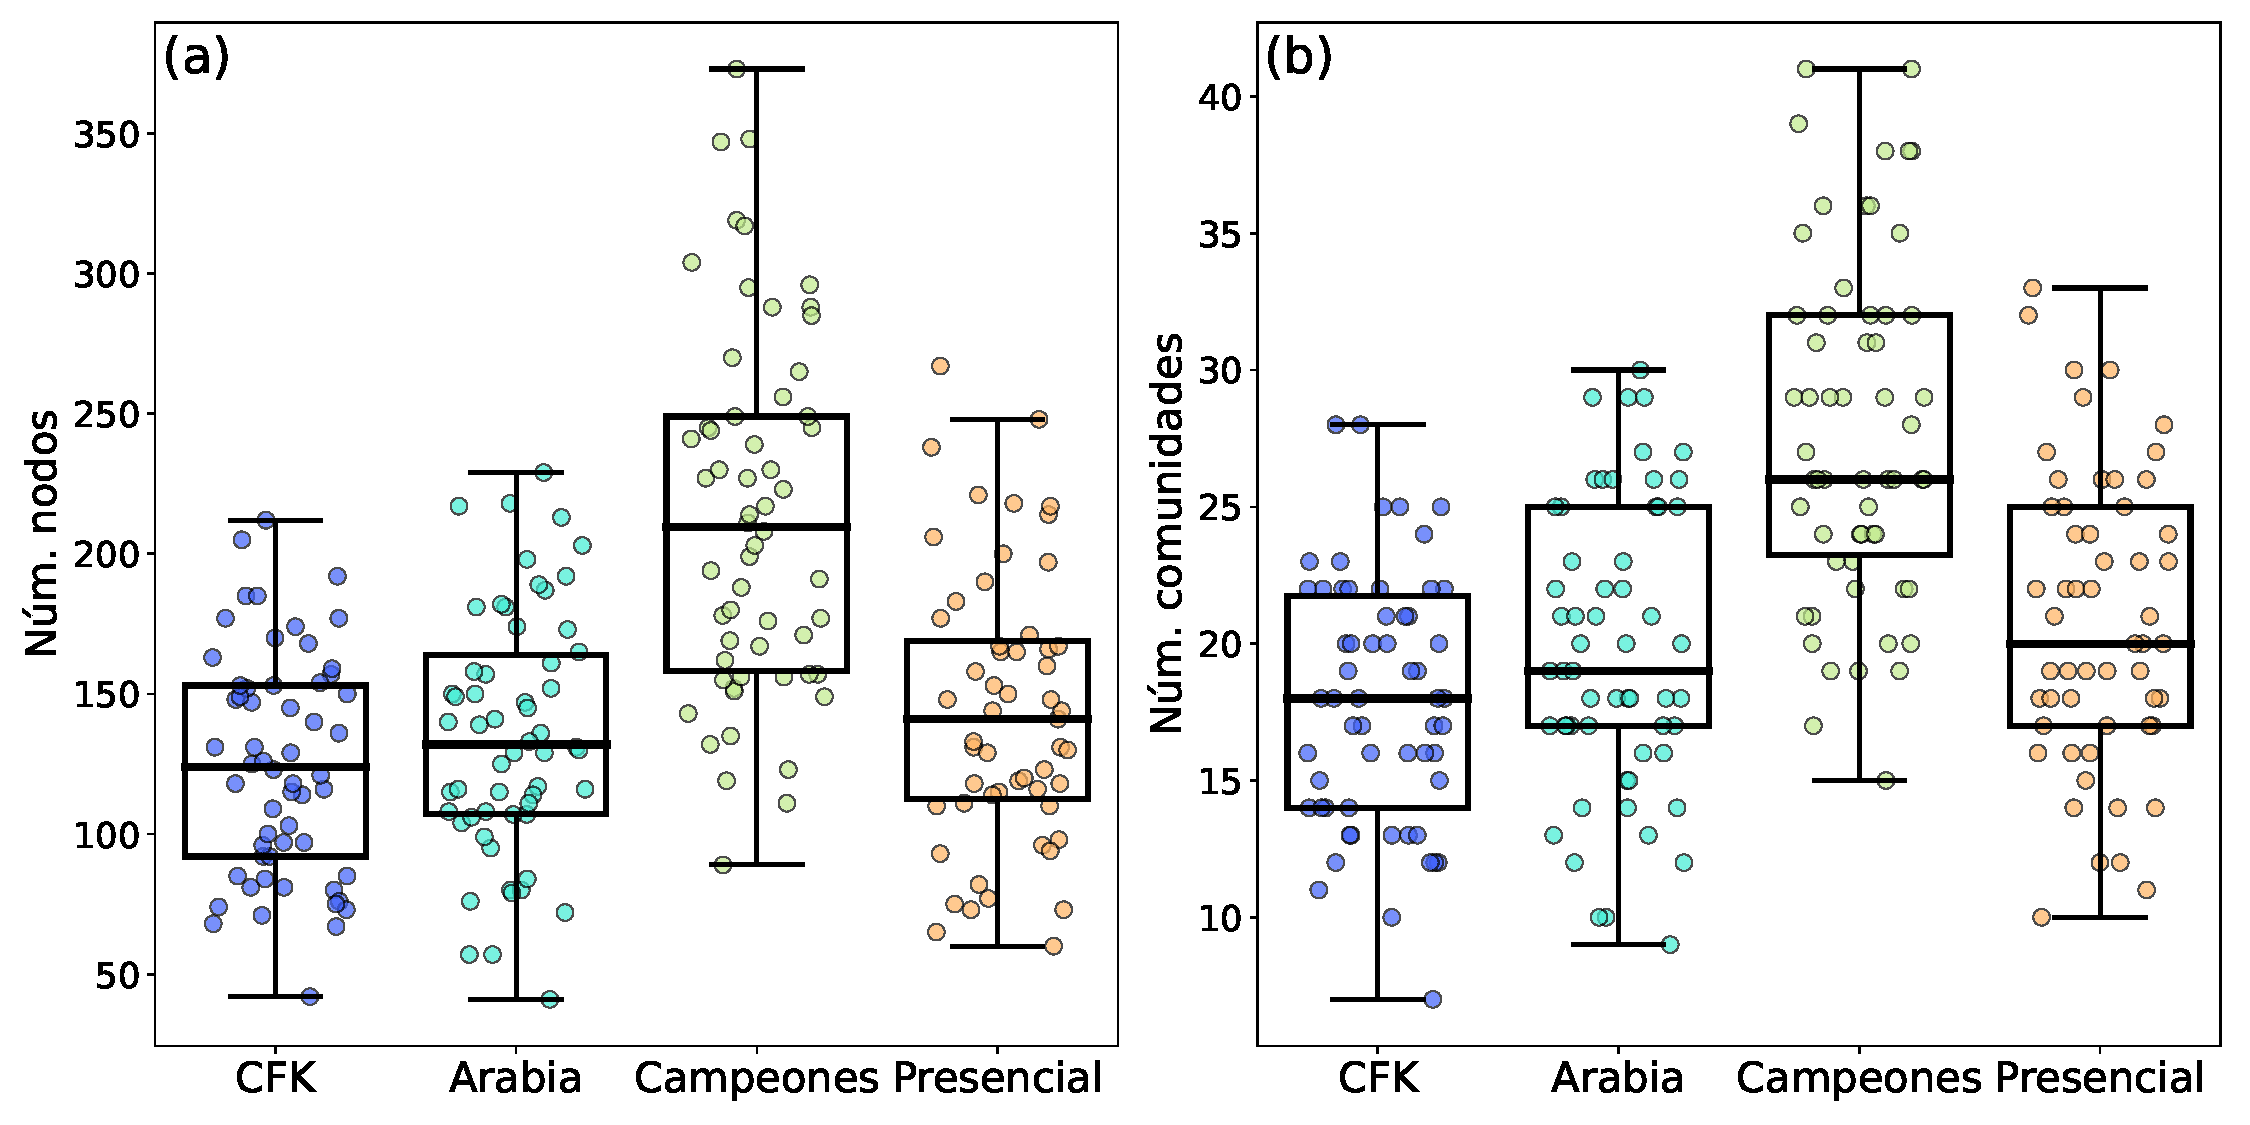
\includegraphics[width = 15cm]{figures/ch03/Herramientas NPL/Primer tiempo/Sin control/estructurales1_boxplot.pdf} 
    \caption{\textbf{(a)}  \textbf{(b)}}
\label{fig:cap3_vars_sentimiento}
\end{figure}


\begin{figure}[H]
    \centering
    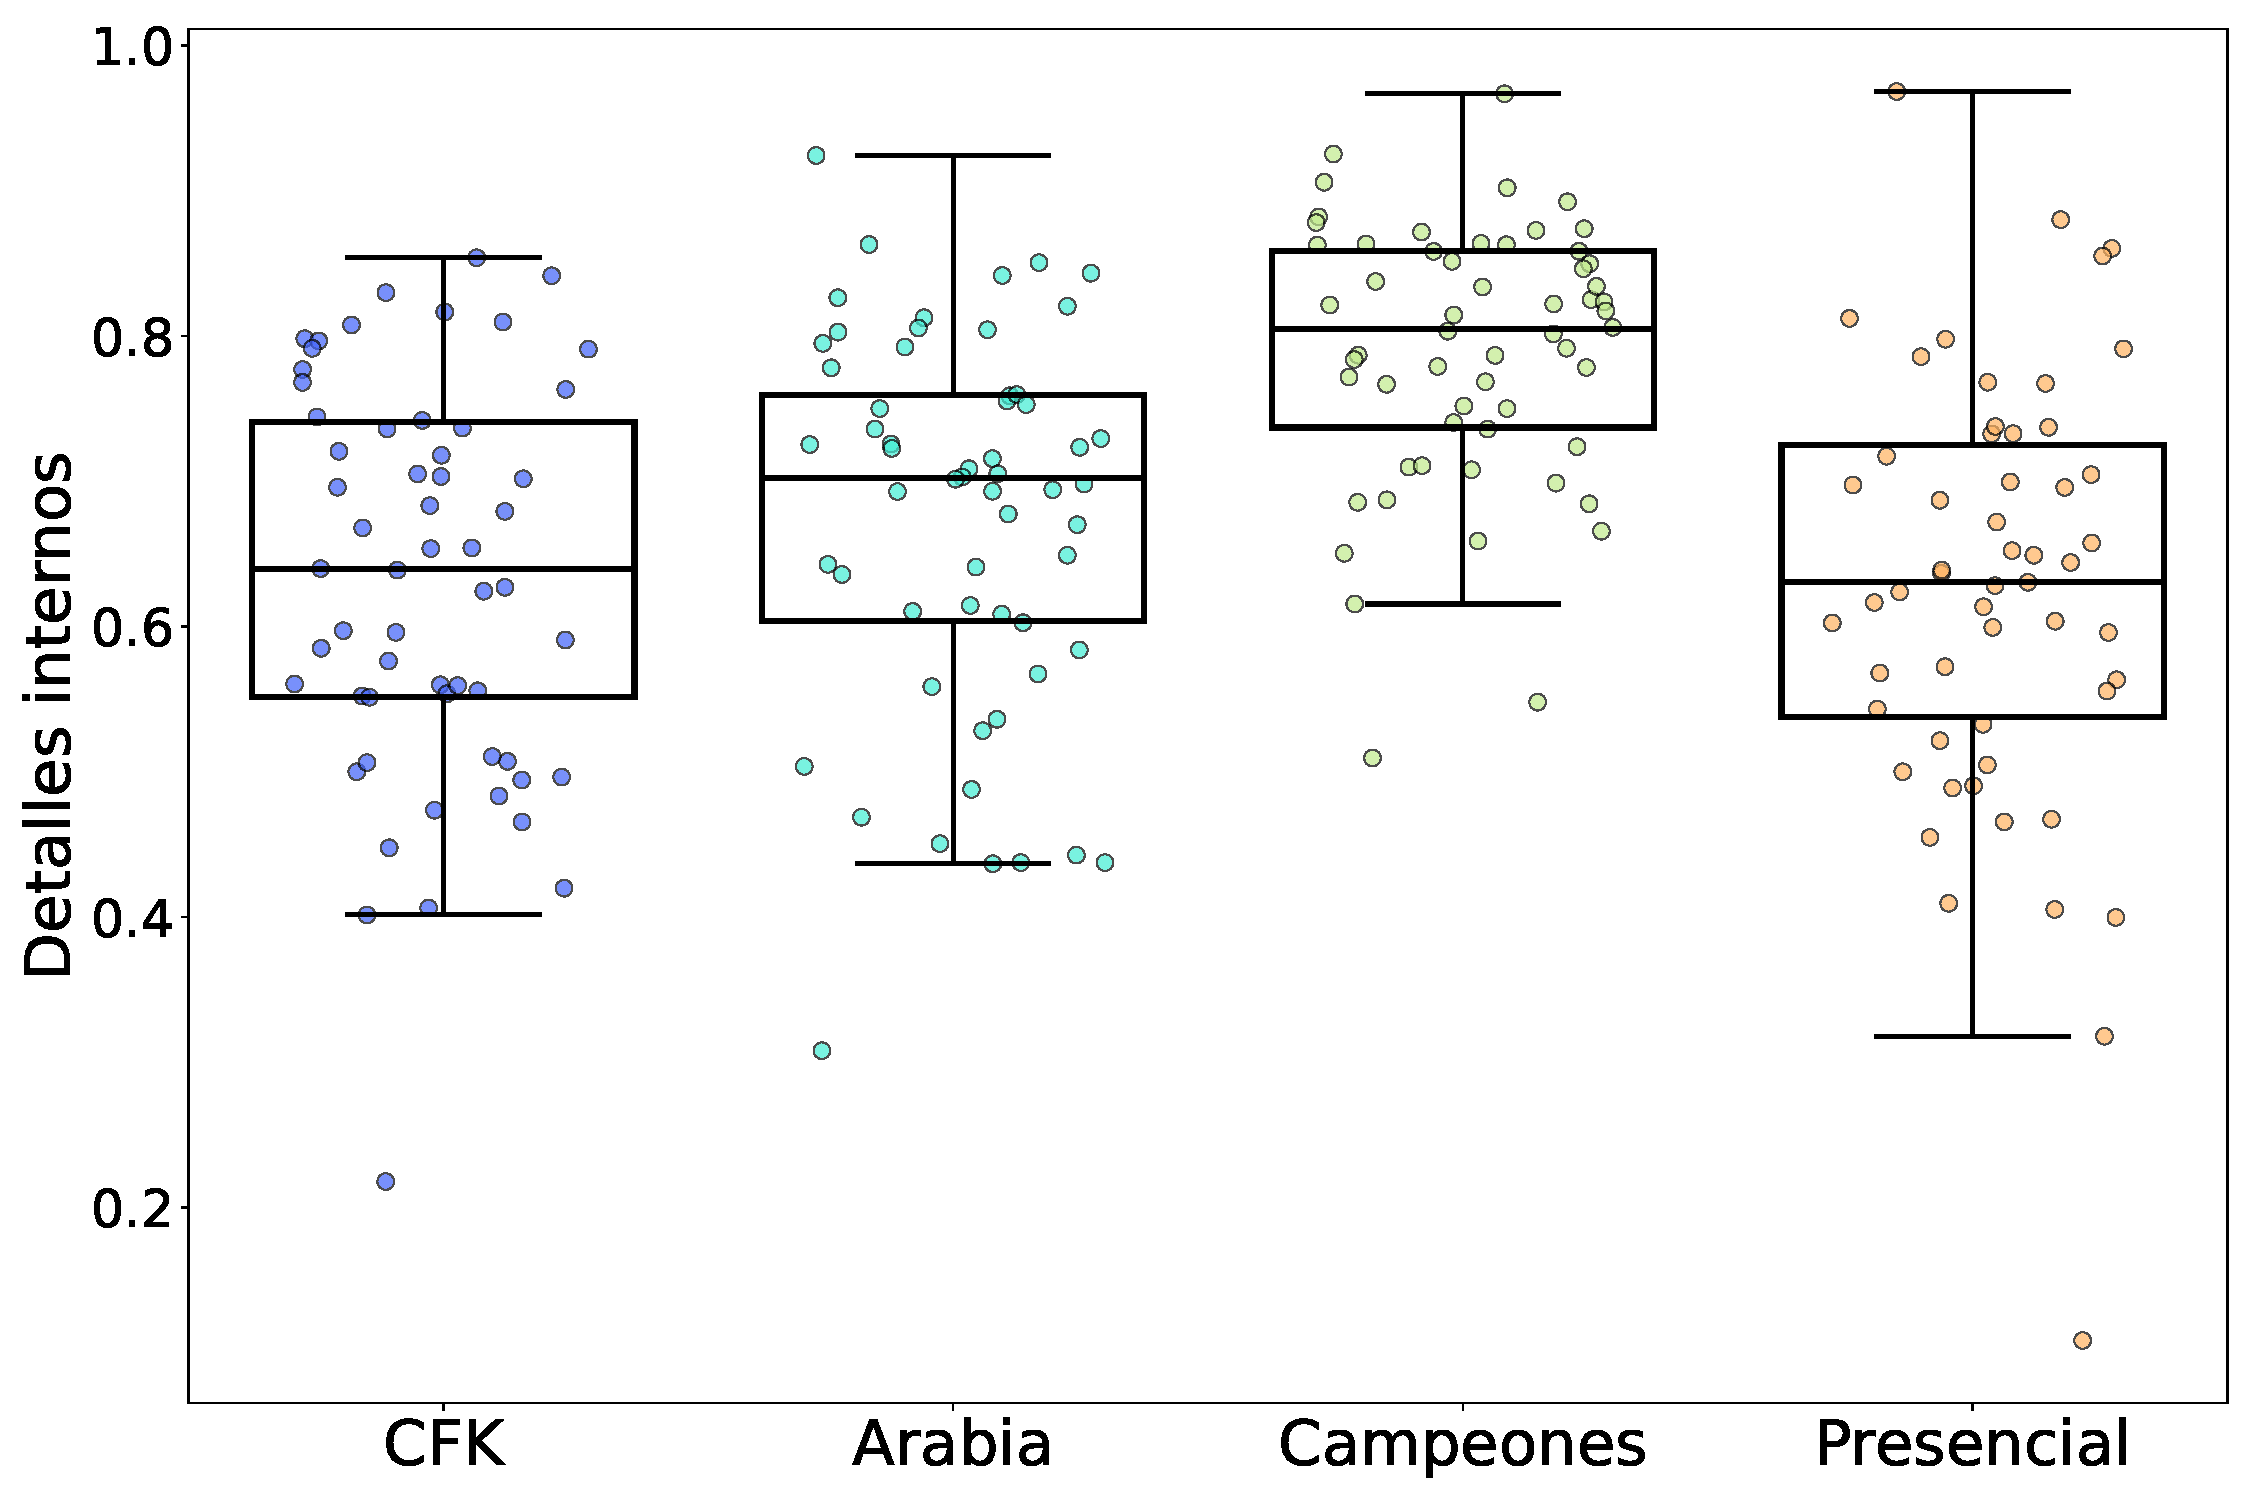
\includegraphics[width = 11cm]{figures/ch03/Herramientas NPL/Primer tiempo/Sin control/memoria_boxplot.pdf} 
    \caption{\textbf{(a)}  \textbf{(b)}}
\label{fig:cap3_var_memoria}
\end{figure}
\end{comment}
Para los cuantificadores de contenido se graficó para cada condición las variables del número de palabras únicas, número de adjetivos y número de pronombres en primera persona como se puede observar en la Figura \ref{fig:cap3_vars_contenido} (a), (b) y (c), respectivamente. Como se observa en la  Figura \ref{fig:cap3_vars_contenido} (a) los participantes hablaron en promedio en la condición campeones, el cual era el relato mas intenso en la validación externa. Luego en presencial hablaron como en su media, y en CFK y Arabia hablaron por debajo de su media. El análisis de ANOVA reportó que hay diferencias significativas entre las medias de los grupos (F$_{3, 138}$ = 61,45, p $<$ 3$\times$10$^{-25}$, $\eta_g^2$ = 0,56). El posterior análisis de Tuckey encontró que la diferencia significativa se da entre el grupo campeones con los demás, en todos los casos con p $<$ 9$\times$10$^{-15}$. \colorbox{yellow}{tengo que aclarar que usé oneway anova en métodos, pero cómo se dice oneway anova en español?, y no debería chequear que los datos sigan una distribución normal?} 
\colorbox{yellow}{aclarar en métodos que se tuvo en cuenta corrección al pval para pasar significancia de tuckey por repetir con varios grupos}
Para el número de adjetivos se observa en la Figura \ref{fig:cap3_vars_contenido}(b) el mayor uso en la condición presencial y el menor uso en la condición de CFK, se hallaron diferencias significativas entre las medias de los grupos (F$_{3, 138}$ = 20,16, p $<$ 7$\times$10$^{-11}$, $\eta_g^2$ = 0,22), en particular entre presencial y CFK con todos las demás condiciones y entre ellas (p $<$ 3$\times$10$^{-3}$). 
Para finalizar con las variables de contenido se graficó el número de palabras en primera persona en la Figura \ref{fig:cap3_vars_contenido}(c). Se puede observar que presencial por mas que es el único relato no colectivo \colorbox{yellow}{hablar de relatos colectivos en intro} es el que menor cantidad de pronombres de primera persona tiene. Del análisis de ANOVA se obtienen diferencias significativas entre las medias (F$_{3, 138}$ = 14,74, p $<$ 3$\times$10$^{-8}$, $\eta_g^2$ = 0,17). El posterior análisis de Tuckey dió que las diferecias son entre la condición presencial con las demás tres condiciones ( p $<$ 4$\times$10$^{-5}$).

\begin{figure}[H]
    \centering
    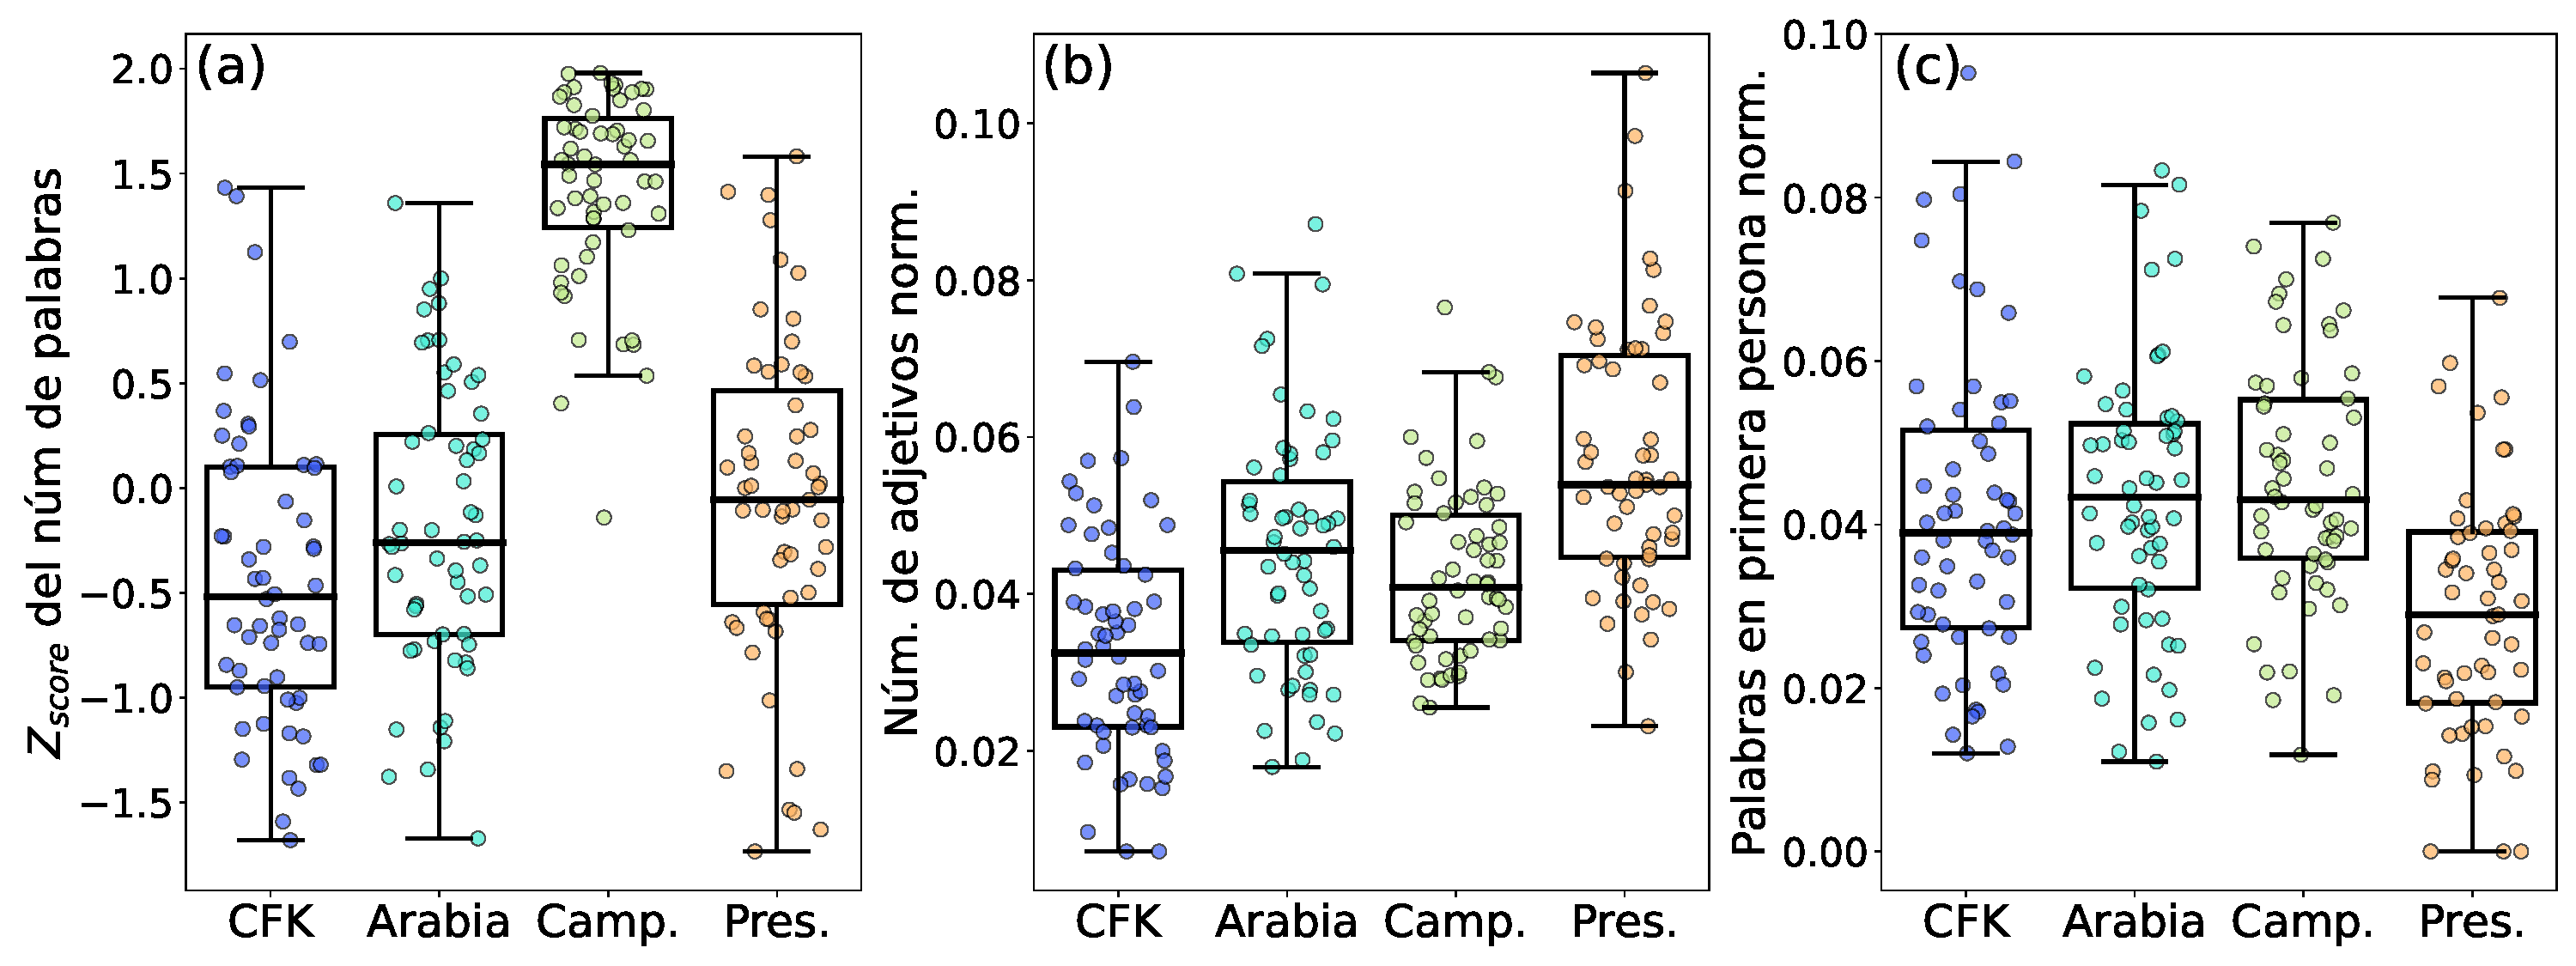
\includegraphics[width = 15cm]{figures/ch03/Herramientas NPL/Primer tiempo/Sin control/contenido_op2_boxplot.pdf} 
    \caption{Boxplots para las distintas condiciones para variables de contenido. En particular en \textbf{(a)} el número de palabras únicas normalizadas con el $Z_{score}$ con los relatos de un mismo sujeto en las diferentes condiciones,  \textbf{(b)} el número de adjetivos normalizado por el número de palabras totales del relato, \textbf{(c)} el número de palabras en primera persona normalizado por el número de palabras en el relato.}
\label{fig:cap3_vars_contenido}
\end{figure}

Continuando con los cuantificadores de sentimiento se graficó en la Figura \ref{fig:cap3_sent_barras} la probabilidad promedio (entre todos los sujetos) de que una condición sea positiva, negativa o intensa (la suma de las dos anteriores). Se puede observar que solo hay diferencias significativas en la intensidad para la condición de presencial respecto de las otras tres, siendo este el menos intenso de todos los relatos. En tanto a la probabilidad de que el relato sea negativo, no se obtuvo diferencia significativas entre las condiciones de CFK y Arabia, ni entre las condiciones de campeones con presencial. Se obtuvo que el primer par son las condiciones mas negativas. Por último la probabilidad de que el relato sea positivo solo no dio diferencias significativas entre las condiciones de Arabia y presencial. Se obtuvo que el relato mas positivo es campeones y el menos positivo es CFK.

\begin{figure}[H]
    \centering
    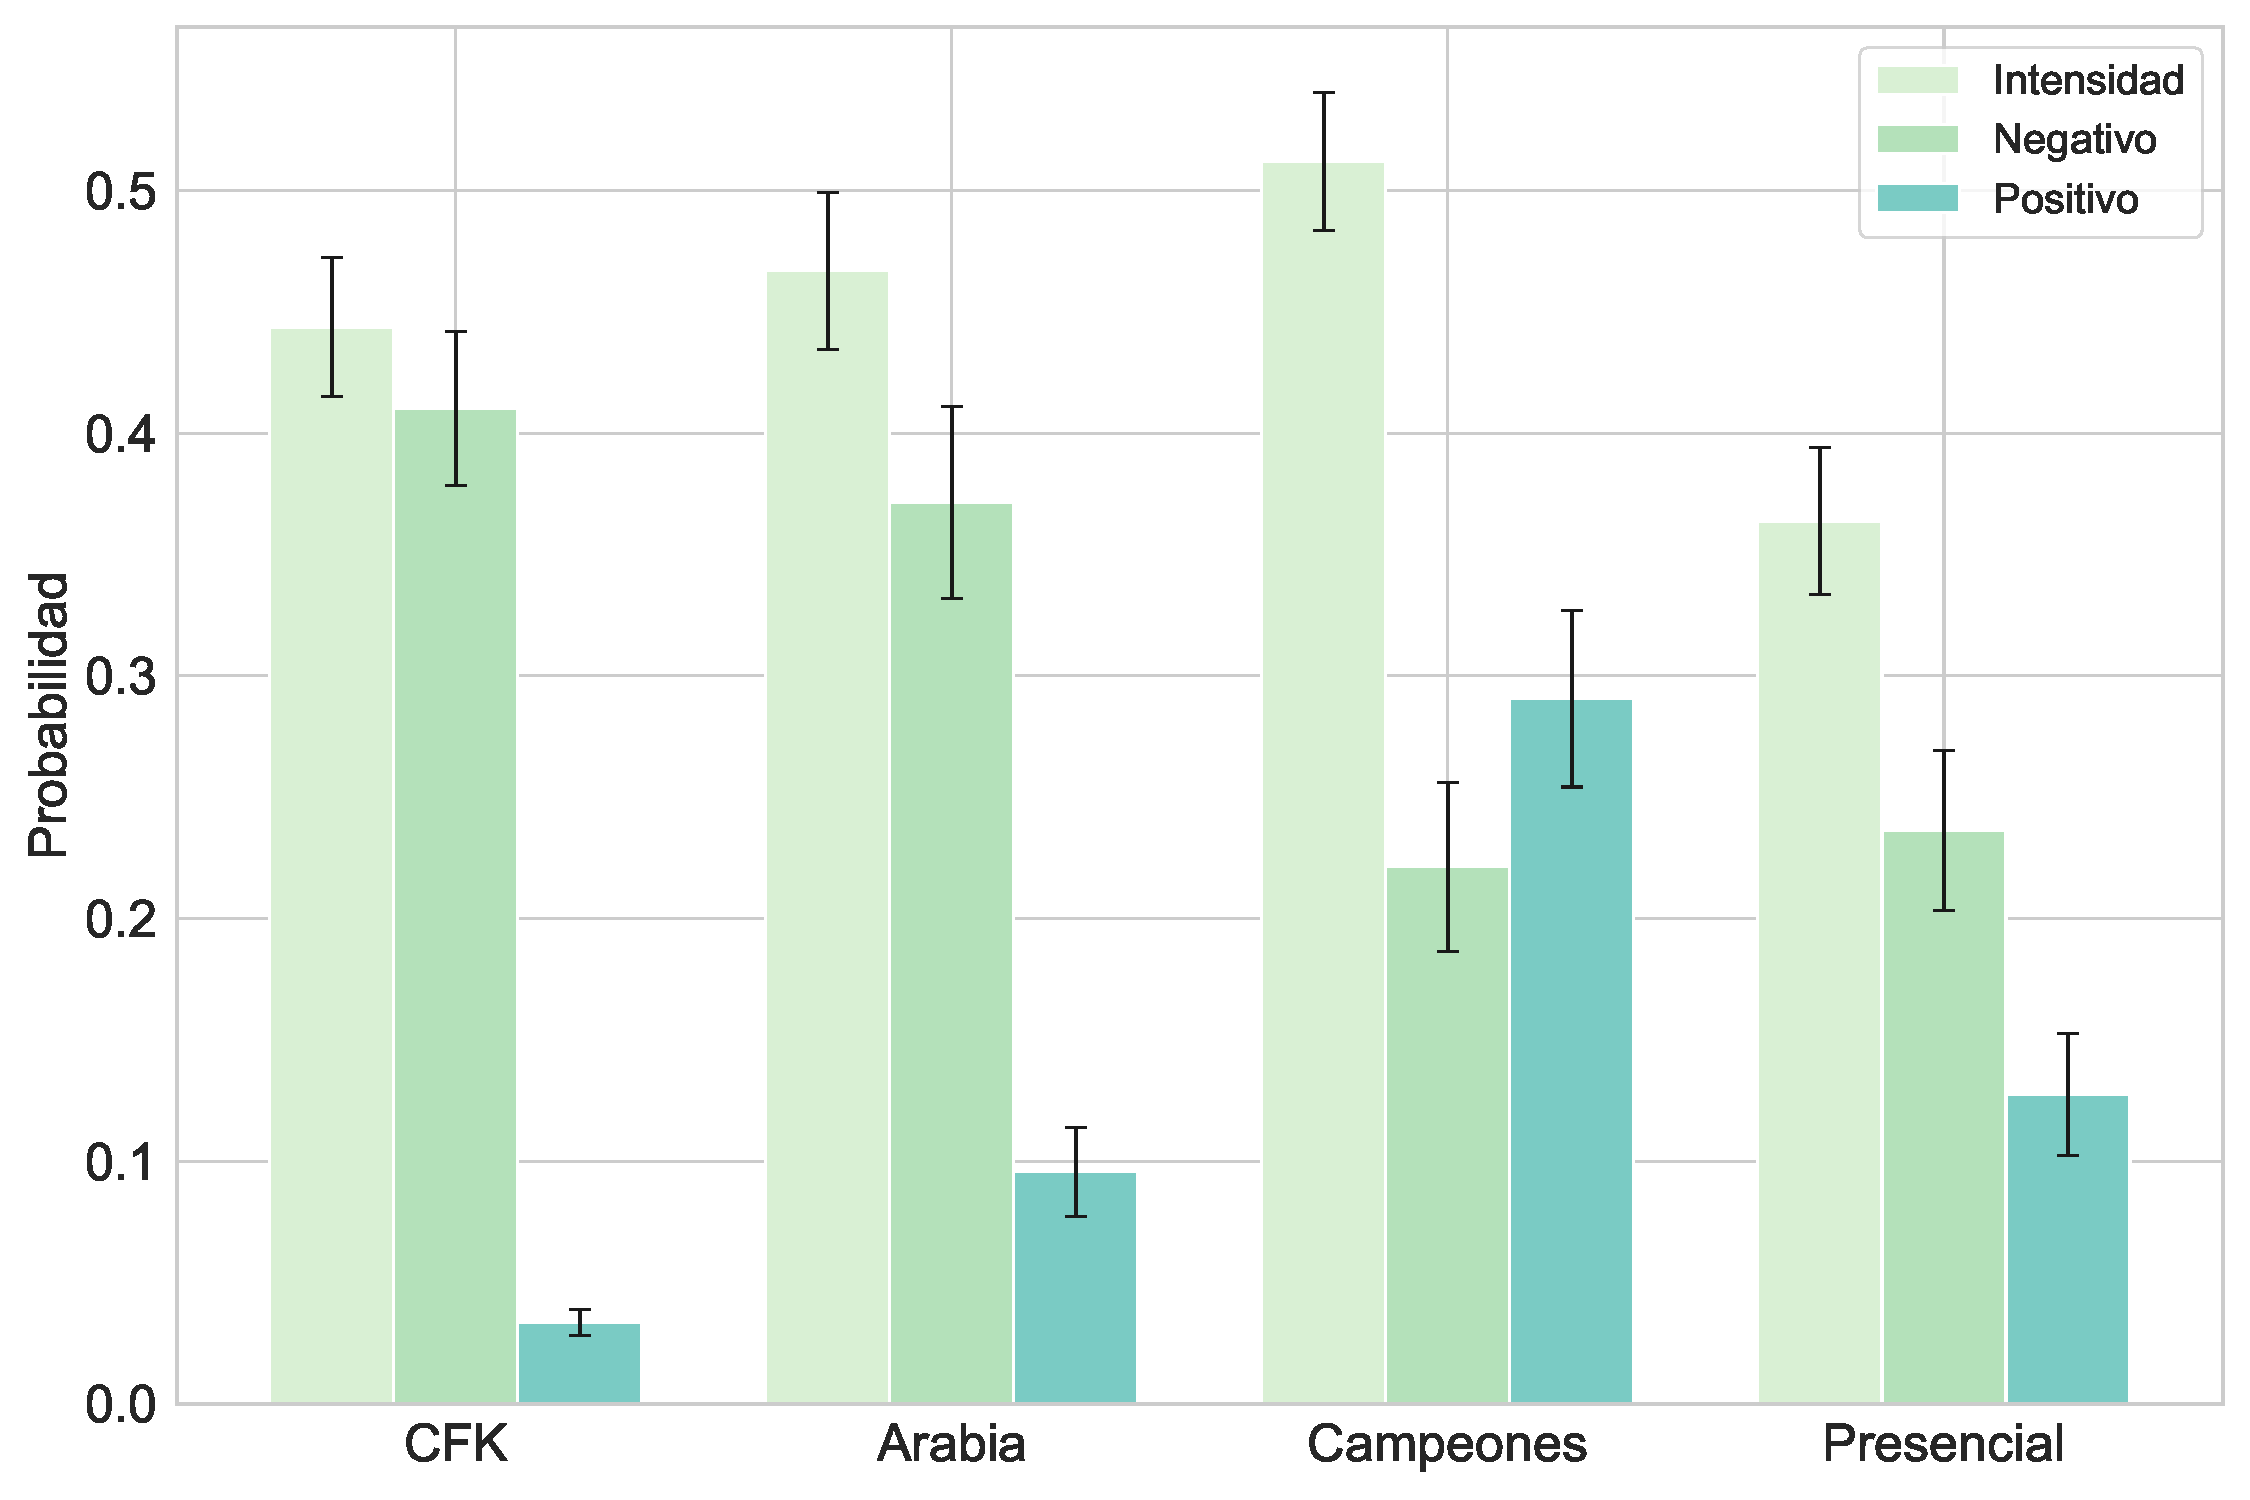
\includegraphics[width = 15cm]{figures/ch03/Herramientas NPL/Primer tiempo/Sin control/pysentimiento_tresbarras.pdf} 
    \caption{Gráfico de la probabilidad de promedio (entre sujetos) de que las condiciones sean positivas negativas o intensas (la suma de las últimas dos) dado de las herramientas de NPL. Estos cuantificadores fueron obtenidos como se indica en \colorbox{yellow}{citar métodos donde explique esto}.}
\label{fig:cap3_sent_barras}
\end{figure}

Luego se realizaron boxplots para algunas de los cuantificadores de sentimiento, los mismos se pueden observar en la Figura \ref{fig:cap3_vars_sentimiento}. En particular, en la Figura \ref{fig:cap3_vars_sentimiento}(a) se observa la variable que denota la probabilidad de que un realto sea positivo. Al igual que se observaba en la Figura \ref{fig:cap3_sent_barras} se tiene que condición mas positiva es campeones y la menos positiva CFK. Existen diferencias significativas entre las medias de los grupos (F$_{3, 138}$ = 16,55, p $<$ 9$\times$10$^{-7}$, $\eta_g^2$ = 0,21) en particular entre campeones y CFK con las otras dos condiciones y entre ellas ( p $<$ 3$\times$10$^{-3}$).

Luego en la Figura \ref{fig:cap3_vars_sentimiento}(b) se observa los boxplots de la variable de intensidad y valencia para las cuatro condiciones. En la misma se puede observar una alta probabilidad densidad de puntos en el cero que denota los relatos que tenian mayor probabilidad de ser neutros. Luego se puede ver que campeones es la condición con mayor cantidad de relatos positivos, sin embargo su mediana al igual que la de presencial es nula. Para los relatos de CFK y Arabia se obtienen medianas negativas. El análisis de ANOVA dió que hay diferencias significativas entre las medias (F$_{3, 138}$ = 10,11, p $<$ 5$\times$10$^{-6}$, $\eta_g^2$ = 0,14) y el posterior analisis de Tuckey reveló que las mismas son entre la condición campeones con CFK y Arabia ( p $<$ 0,0014) y entre CFK y presencial (p $<$ 0,0006).

El último cuantificador de sentimiento graficado es la intensidad y se observa en la Figura \ref{fig:cap3_vars_sentimiento}(c), al igual que como se obserba en la Figura \ref{fig:cap3_sent_barras} la condición menos intensa resulta ser presencial. El análisis de ANOVA muestra diferencia significativa entre las medias (F$_{3, 138}$ = 3,64, p $<$ 0,01, $\eta_g^2$ = 0,05), la prueba de Tuckey muestra que la diferencia significativa se da entre las condiciones campeones y presencial (p $<$ 0.0035).

\begin{figure}[H]
    \centering
    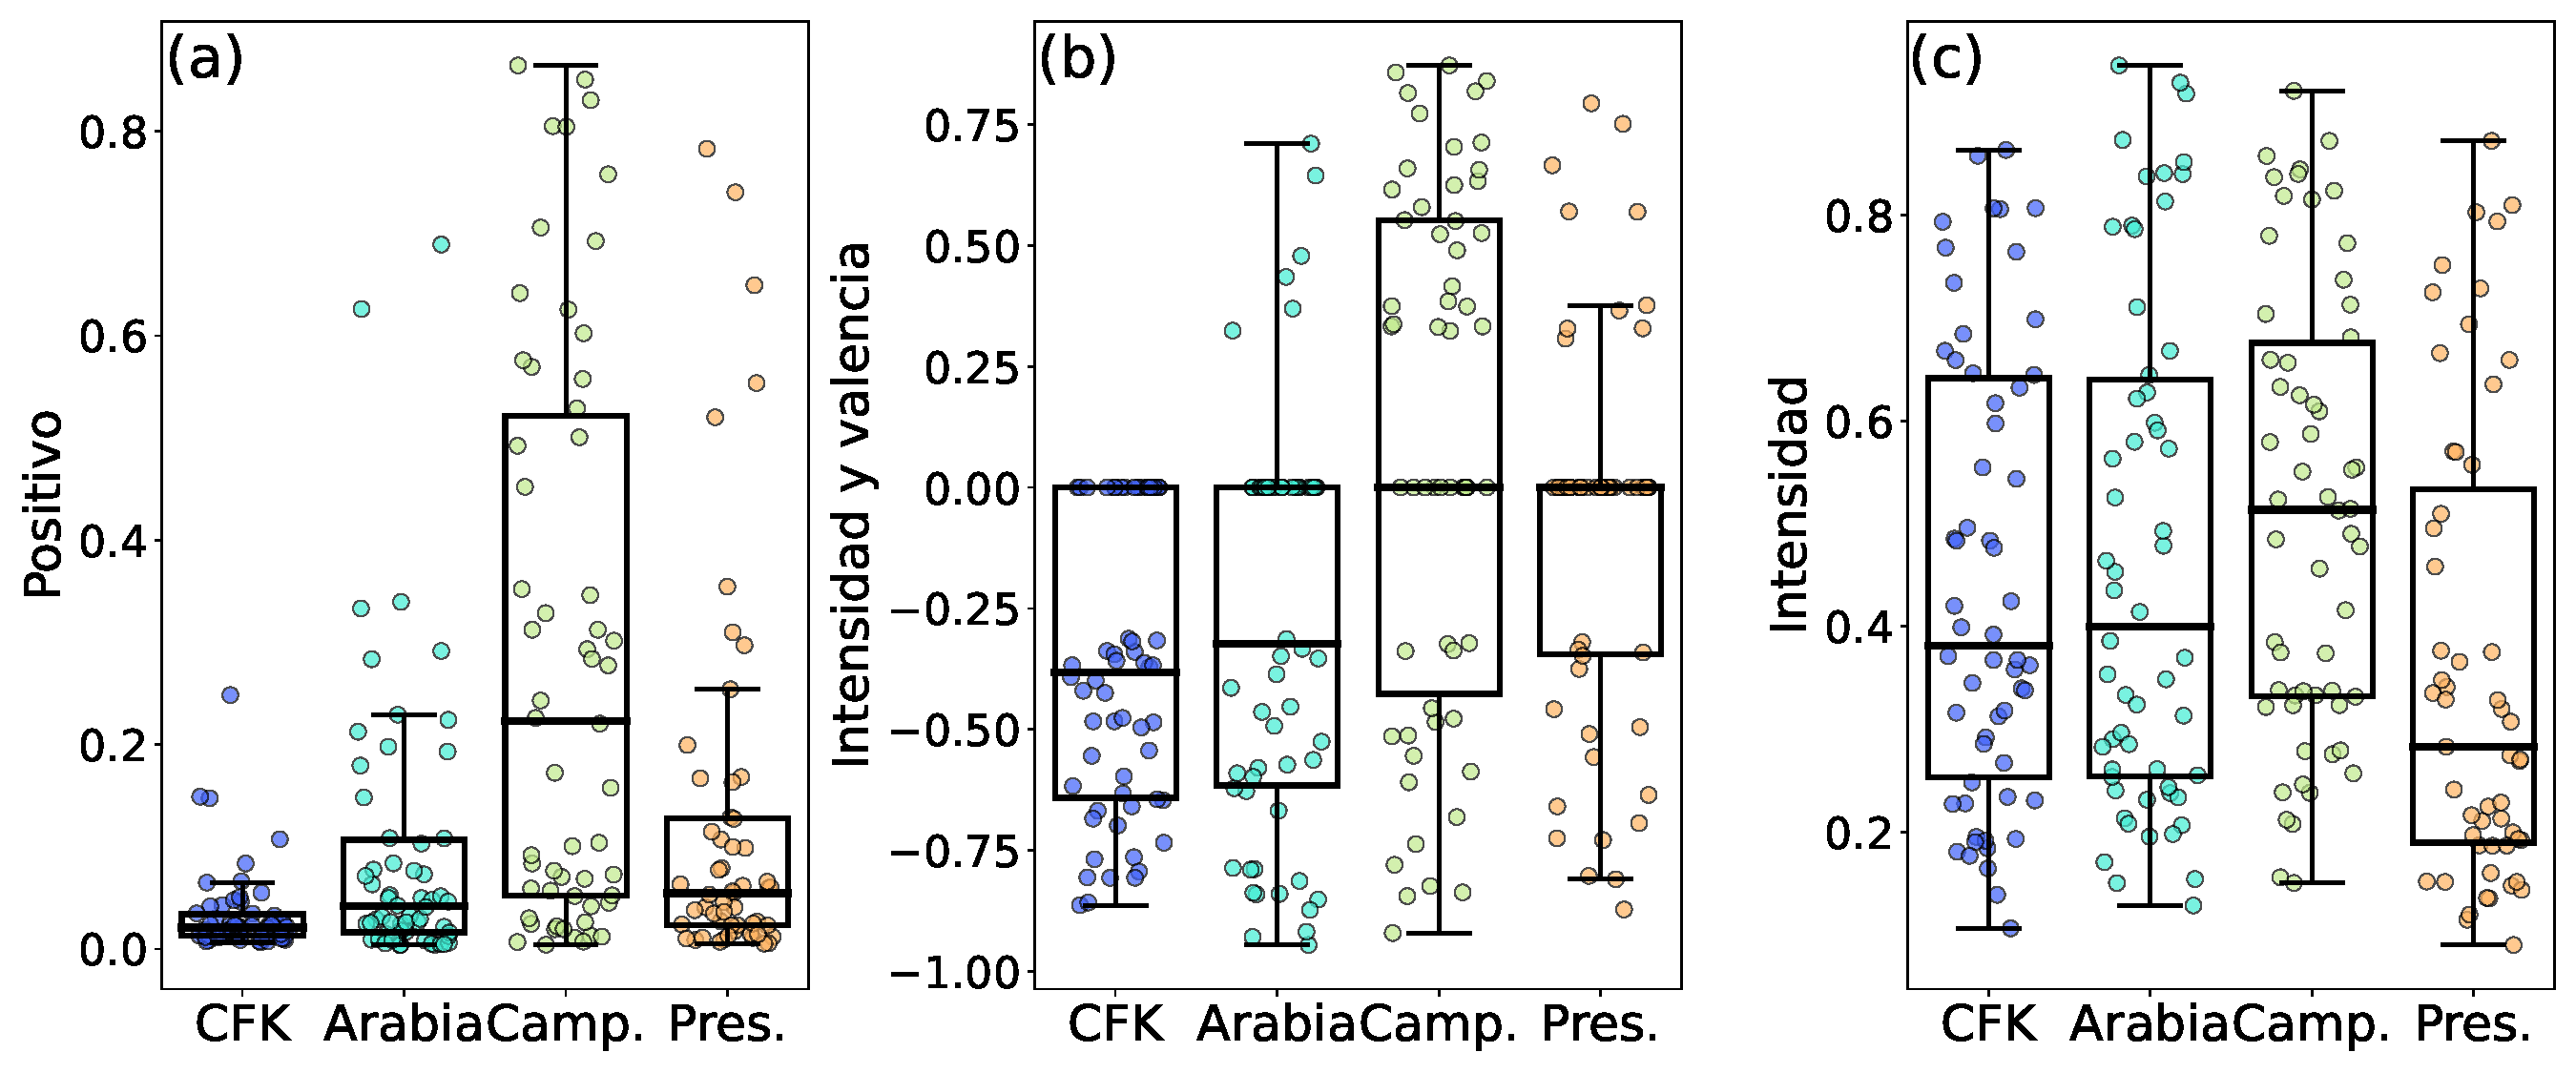
\includegraphics[width = 15cm]{figures/ch03/Herramientas NPL/Primer tiempo/Sin control/sentimiento_op2_boxplot.pdf} 
    \caption{Boxplots para las distintas condiciones para variables de sentimiento. En particular en \textbf{(a)} la probabilidad de que el relato sea positivo. En \textbf{(b)} la valencia por la intensidad. En \textbf{(c)} la intensidad del relato (suma de la probabilidad de negativo mas positivo).}
\label{fig:cap3_vars_sentimiento}
\end{figure}

Continuando con las variables estructurales, inicialmente se observó si la coherencia disminuye con la distancia entre las oraciones al calcularla. Se construyó un modelo nulo promedio como se explicó en \colorbox{yellow}{citar} y se calculó la coherencia promedio entre los sujetos para cada condición. Esto es lo que se puede observar graficado en la Figura \ref{fig:cap3_coherencia_d}, donde la línea punteada negra denota el modelo nulo promedio. Se observa que la coherencia efectivamente disminuye al aumentar la distancia entre oraciones y además se ve un comportamiento sostenido en la distancia donde la coherencia media de la condición Arabia es la mayor y la de presencial la menor. \colorbox{yellow}{Esto podría deberse al hecho de que presencial es el mas lejano en el tiempo, asi como también el menos intenso.}


\begin{figure}[H]
    \centering
    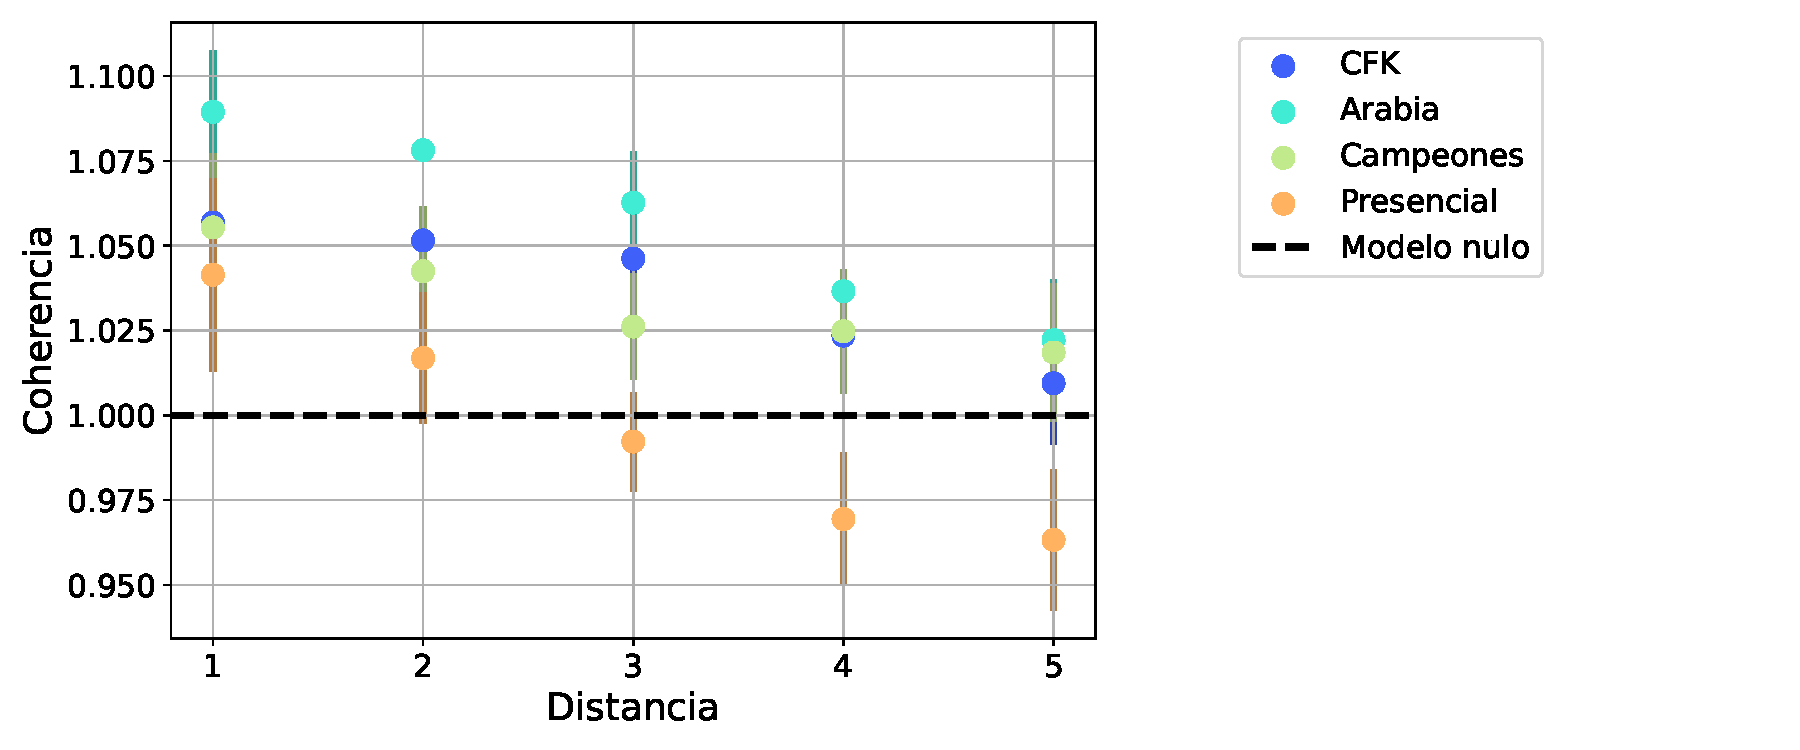
\includegraphics[width = 15cm]{figures/ch03/Herramientas NPL/Primer tiempo/Sin control/coherencia_vs_t_conmodelonulo.pdf} 
    \caption{Coherencia promedio (entre los sujetos) para cada condición en función de la distancia entre las oraciones utilizada para calcularla. La linea negra punteada denota el modelo nulo promedio.}
\label{fig:cap3_coherencia_d}
\end{figure}

En la Figura \ref{fig:cap3_vars_estructurales} (a), (b) y (c) se pueden observar tres cuantificadores estructurales. En (a) la coherencia utilizando una distancia de 3 (es decir, calculando la coherencia del relato entre oraciones que se encuentran separadas por tres de ellas). En (b) el número de nodos de la componente fuertemente conexa del grafo hecho a partir del relato, y en (c) el número de comunidades de la misma componente. En la Figura \ref{fig:cap3_vars_estructurales}(a) se puede observar como la coherencia a distancia 3 es similar en todas las condiciones lo cual es confirmado con el análisis de ANOVA con el cual no se obtiene diferencia significativa entre las medias (p = 0,08). Resultados similares se obtienen para distancia 1 y 2. En tanto a las variables que son atributos de la red de grafo armada del relato de los participantes se tiene en todas un F significativo, en particular en en el número de nodos y comunidades en la componente fuertemente conexa como se ve en la Figura \ref{fig:cap3_vars_estructurales}(b) y (c) la condición de campeones tiene una mediana mayor a las demás condiciones, el ANOVA de cada caso es respectivamente F$_{3, 138}$ = 50,18, p $<$ 5,5$\times$10$^{-22}$, $\eta_g^2$ = 0,38 y F$_{3, 138}$ = 42,38,  p $<$ 1,8$\times$10$^{-19}$, $\eta_g^2$ = 0,37. El análisis de Tuckey muestra que en ambos casos la diferencia de la media es de campeones con las otras tres condiciones, en todos los casos con  p $<$ 7,8$\times$10$^{-10}$.
Sin embargo, este no es el comportamiento de todos los atributos de las redes de los relatos, se puede observar en la Figura \ref{fig:cap3_vars_mem}(a) la densidad que tiene un comportamiento contrario donde la condición de campeones tiene menor densidad que las demás (F$_{3, 138}$ = 23,79, p $<$ 1,8$\times$10$^{-12}$, $\eta_g^2$ = 0,27, Tuckey significativo entre campeones y las demás con p $<$ 3,2$\times$10$^{-9}$). O como para el coeficiente de clustering promedio que se observa en la Figura \ref{fig:cap3_vars_mem}(b) y se puede apreciar una menor diferencia entre las medias (F$_{3, 138}$ = 4,6, p $<$ 0,0043, $\eta_g^2$ = 0,06, Tuckey significativo entre campeones y presencial con p = 0,001).


\begin{figure}[H]
    \centering
    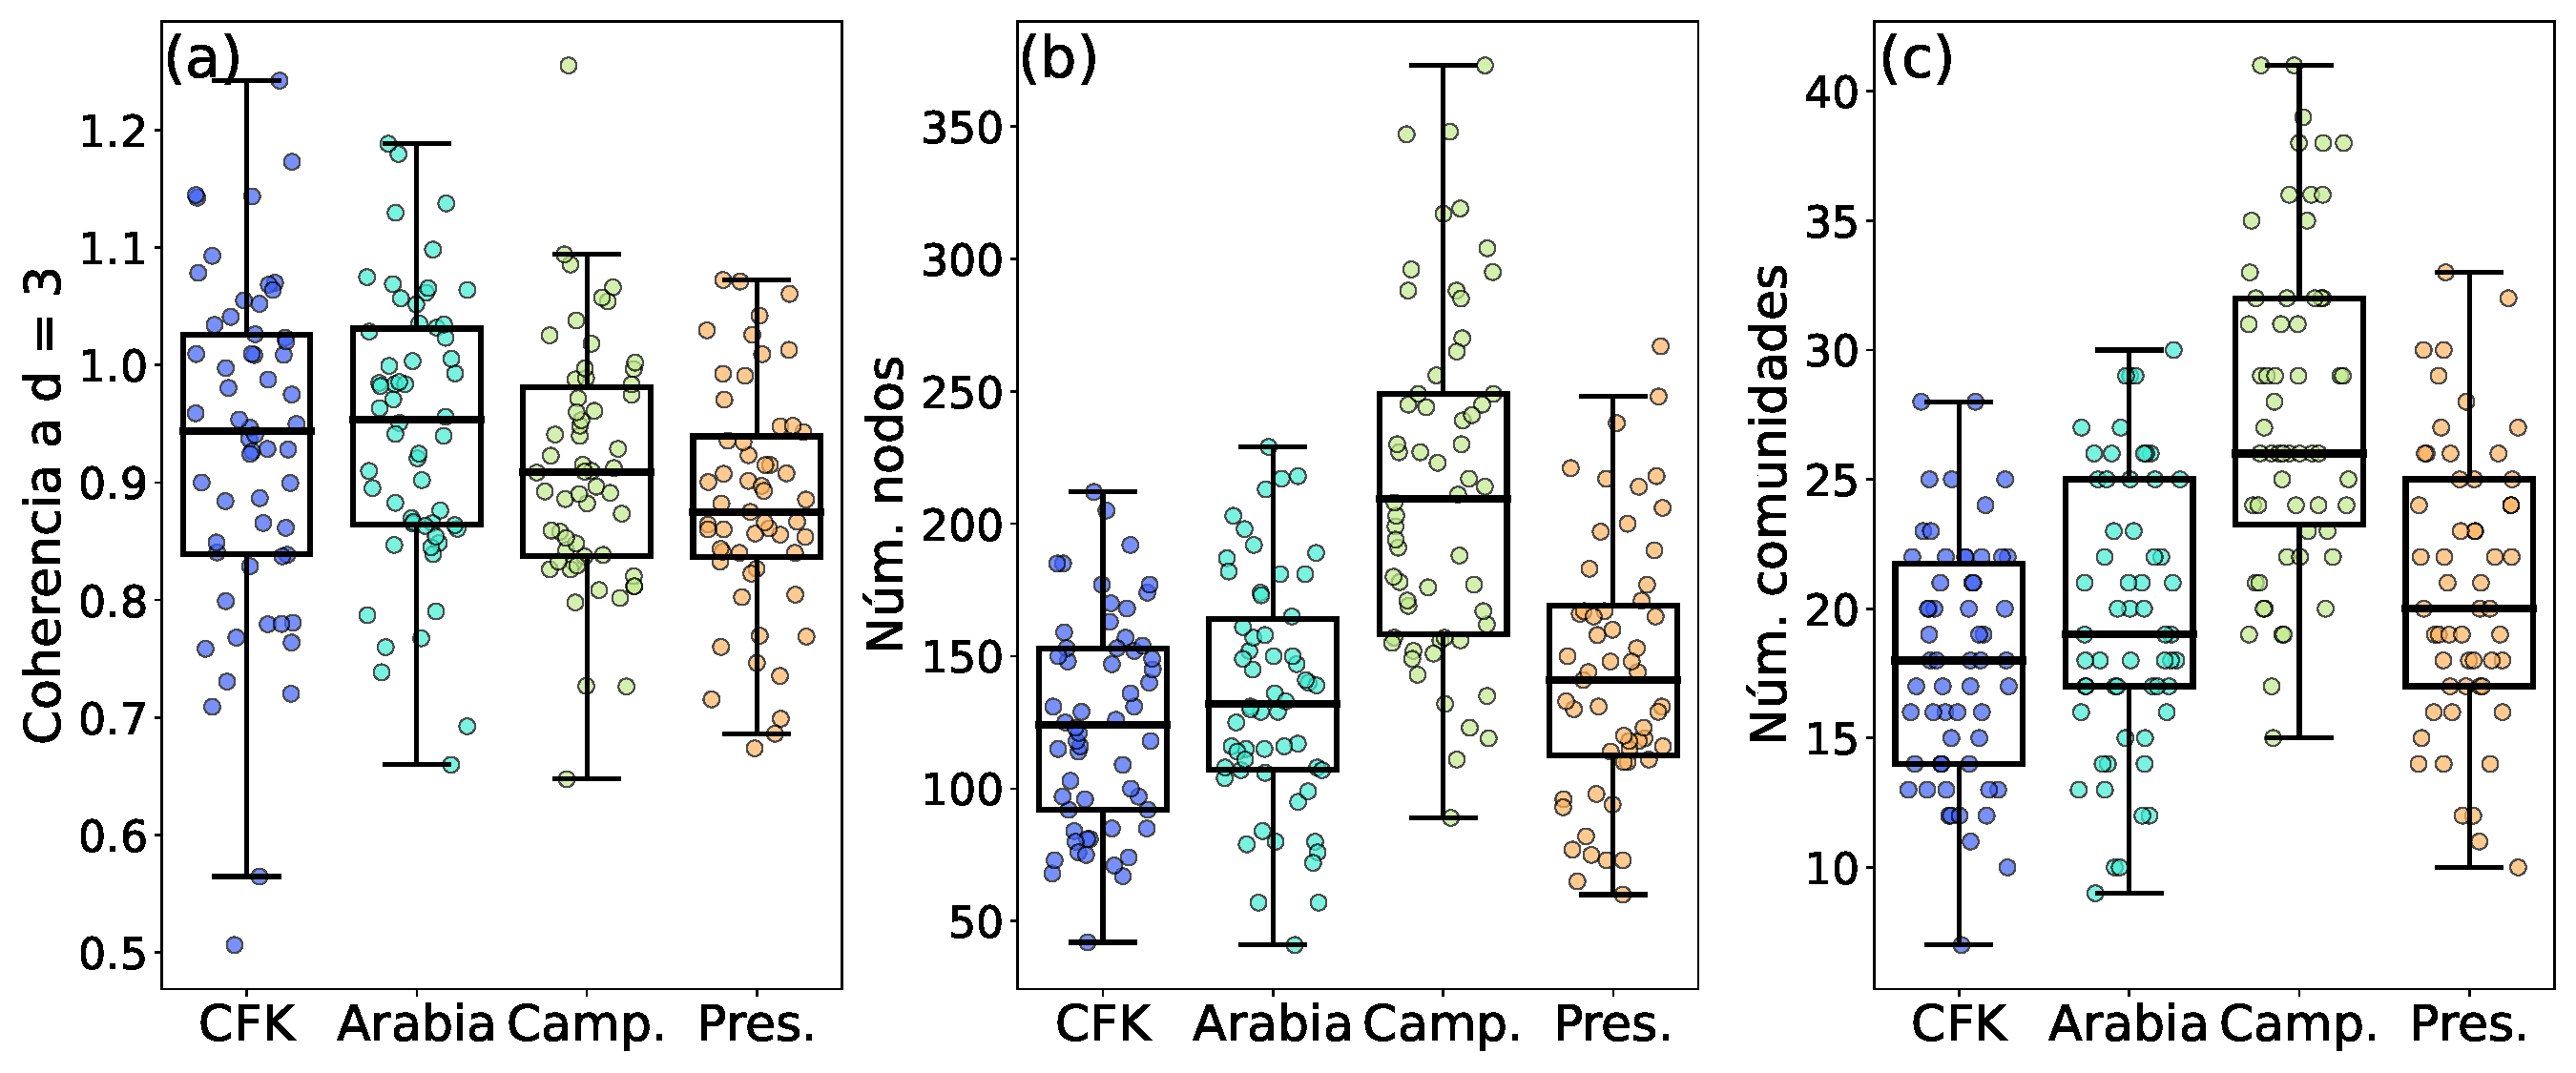
\includegraphics[width = 15cm]{figures/ch03/Herramientas NPL/Primer tiempo/Sin control/estructurales1op2_boxplot.pdf} 
    \caption{Gráfico de boxplot de diferentes variables estructurales para las distintas condiciones. En particular en \textbf{(a)} de la coherencia a distancia 3, en  \textbf{(b)} del número de nodos en la componente fuertemente conexa y en \textbf{(c)} del número de comunidades en la misma componente.}
\label{fig:cap3_vars_estructurales}
\end{figure}

Por último los cuantificadores de memoria que son detalles interno y externos. Como están anticorrelacionados vamos a solo observar el primero en la Figura \ref{fig:cap3_vars_mem}(c). Se puede observar una mayor cantidad de detalles internos en la condición de campeones y la menor en presencial. El ANOVA dio diferencia significativa entre las medias F$_{3, 138}$ = 21,3, p $<$ 2,2$\times$10$^{-11}$, $\eta_g^2$ = 0,22 y Tuckey significativo entre campeones y las demás condiciones con p $<$ 5$\times$10$^{-6}$.


\begin{figure}[H]
    \centering
    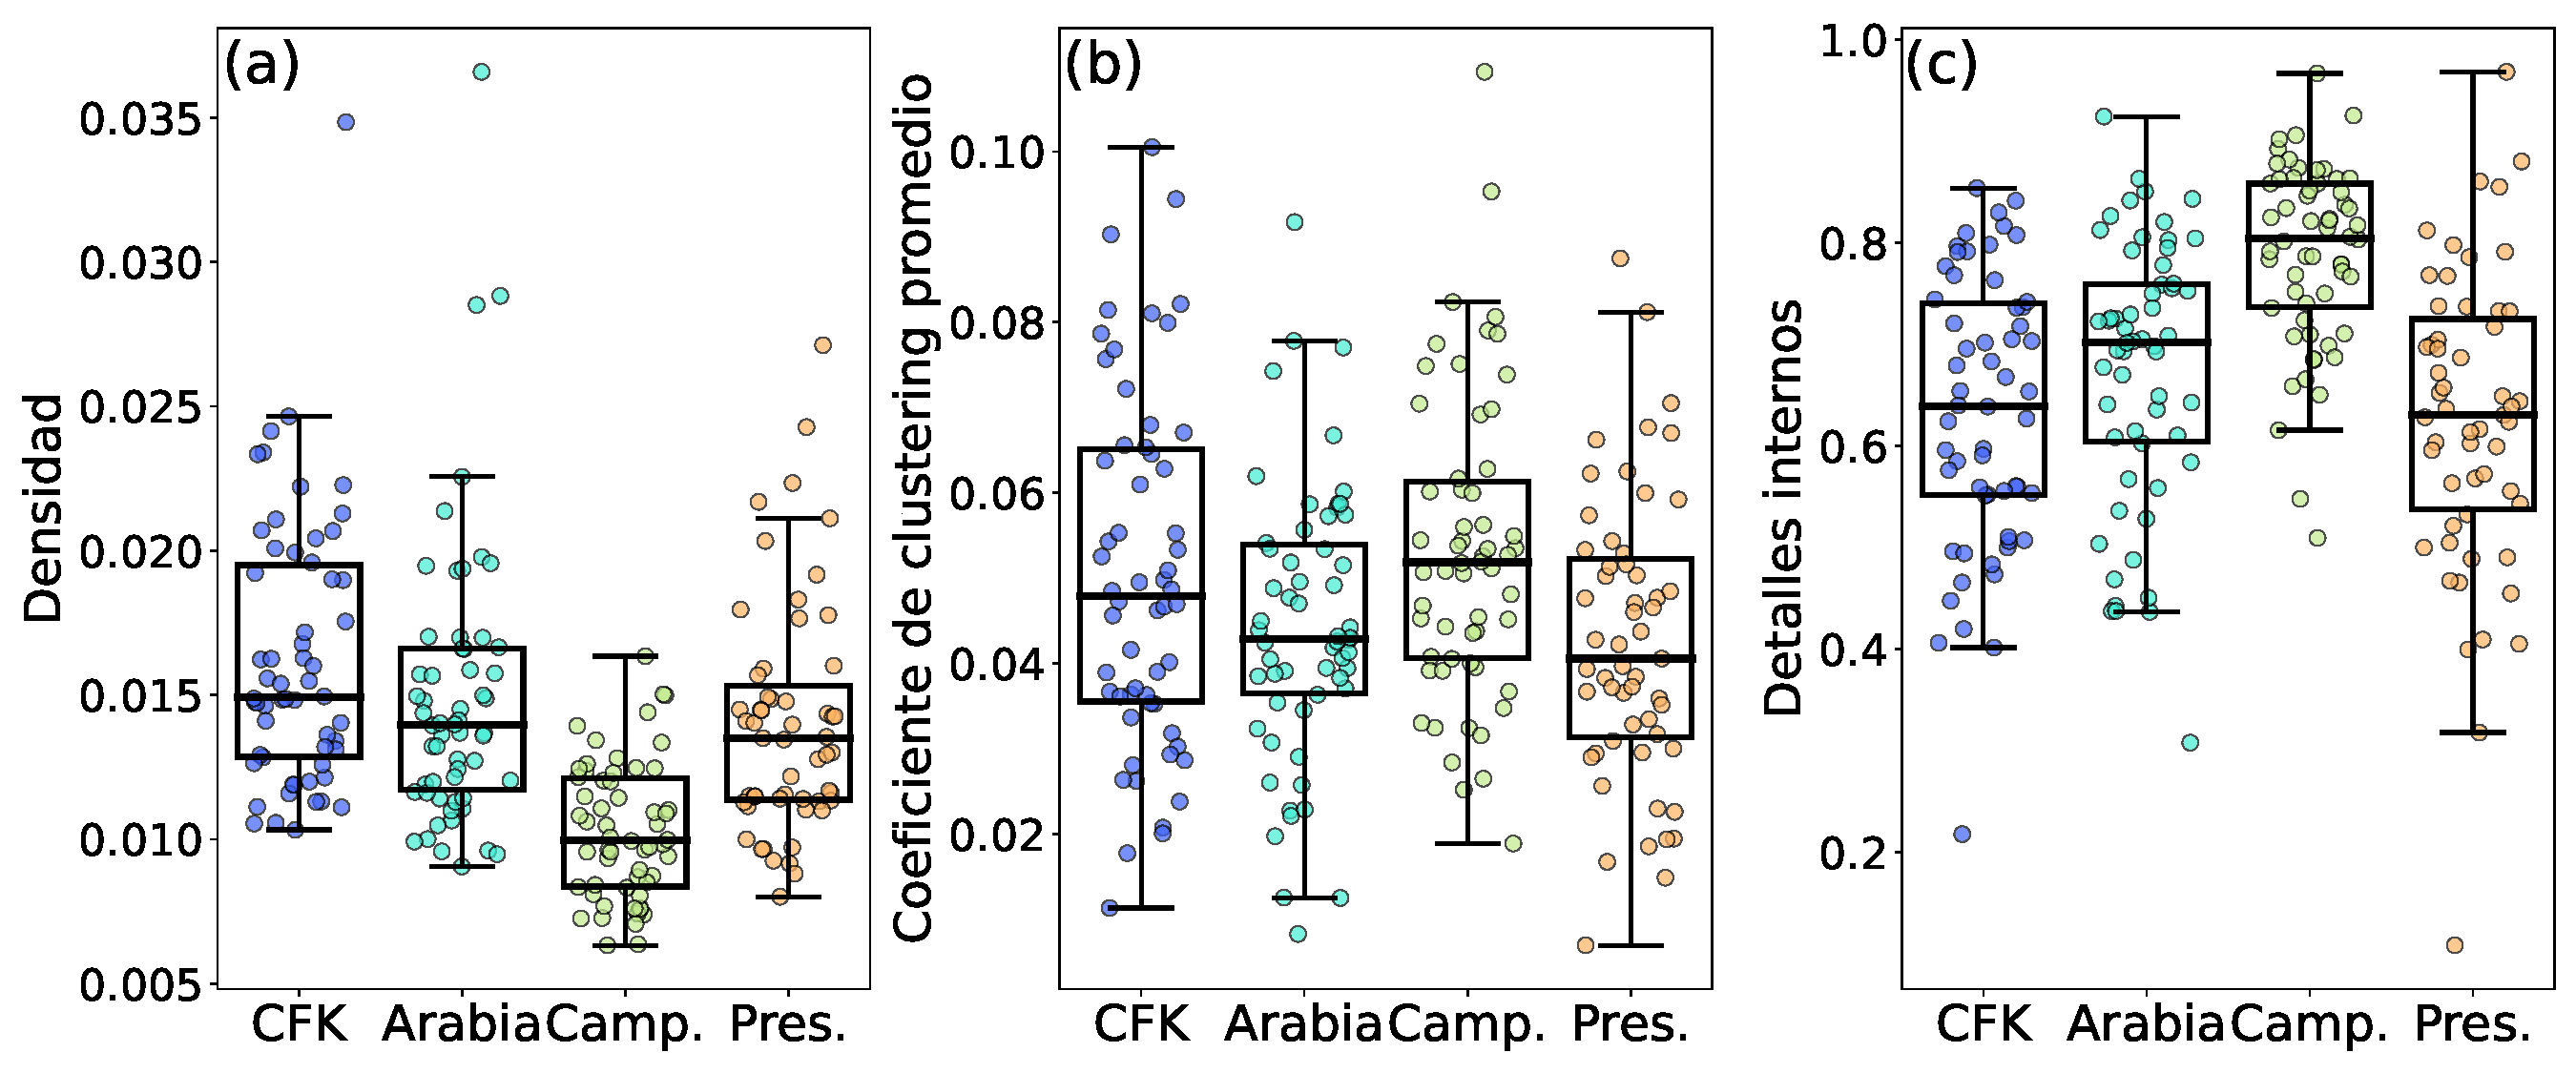
\includegraphics[width = 15cm]{figures/ch03/Herramientas NPL/Primer tiempo/Sin control/estructurales2op2_boxplot.pdf} 
    \caption{Boxplots para las distintas condiciones de variables estructurales y de memoria. En particular en \textbf{(a)} para la densidad de la red armada con los relatos, en \textbf{(b)} del coeficiente de clustering promedio de dicha red y en \textbf{(c)} la variable de memoria de detalles internos.}
\label{fig:cap3_vars_mem}
\end{figure}


\section{Correlación entre las variables del relato y de autopercepción}

Se estudió la correlación entre las variables discursivas incluyendo además las variables obtenidas de las respuestas del cuestionario posterior a la entrevista. Se obtuvo el resultado de la Figura \ref{fig:cap3_corr} para el primer tiempo, donde se grafica la matriz de correlación. El color blanco representa que el p$_{val}$ no fue significativo. Se tuvo en cuenta la corrección por las múltiples comparaciones (¿comparaciones? ¿cálculos?). 


\begin{figure}[h]
    \centering
    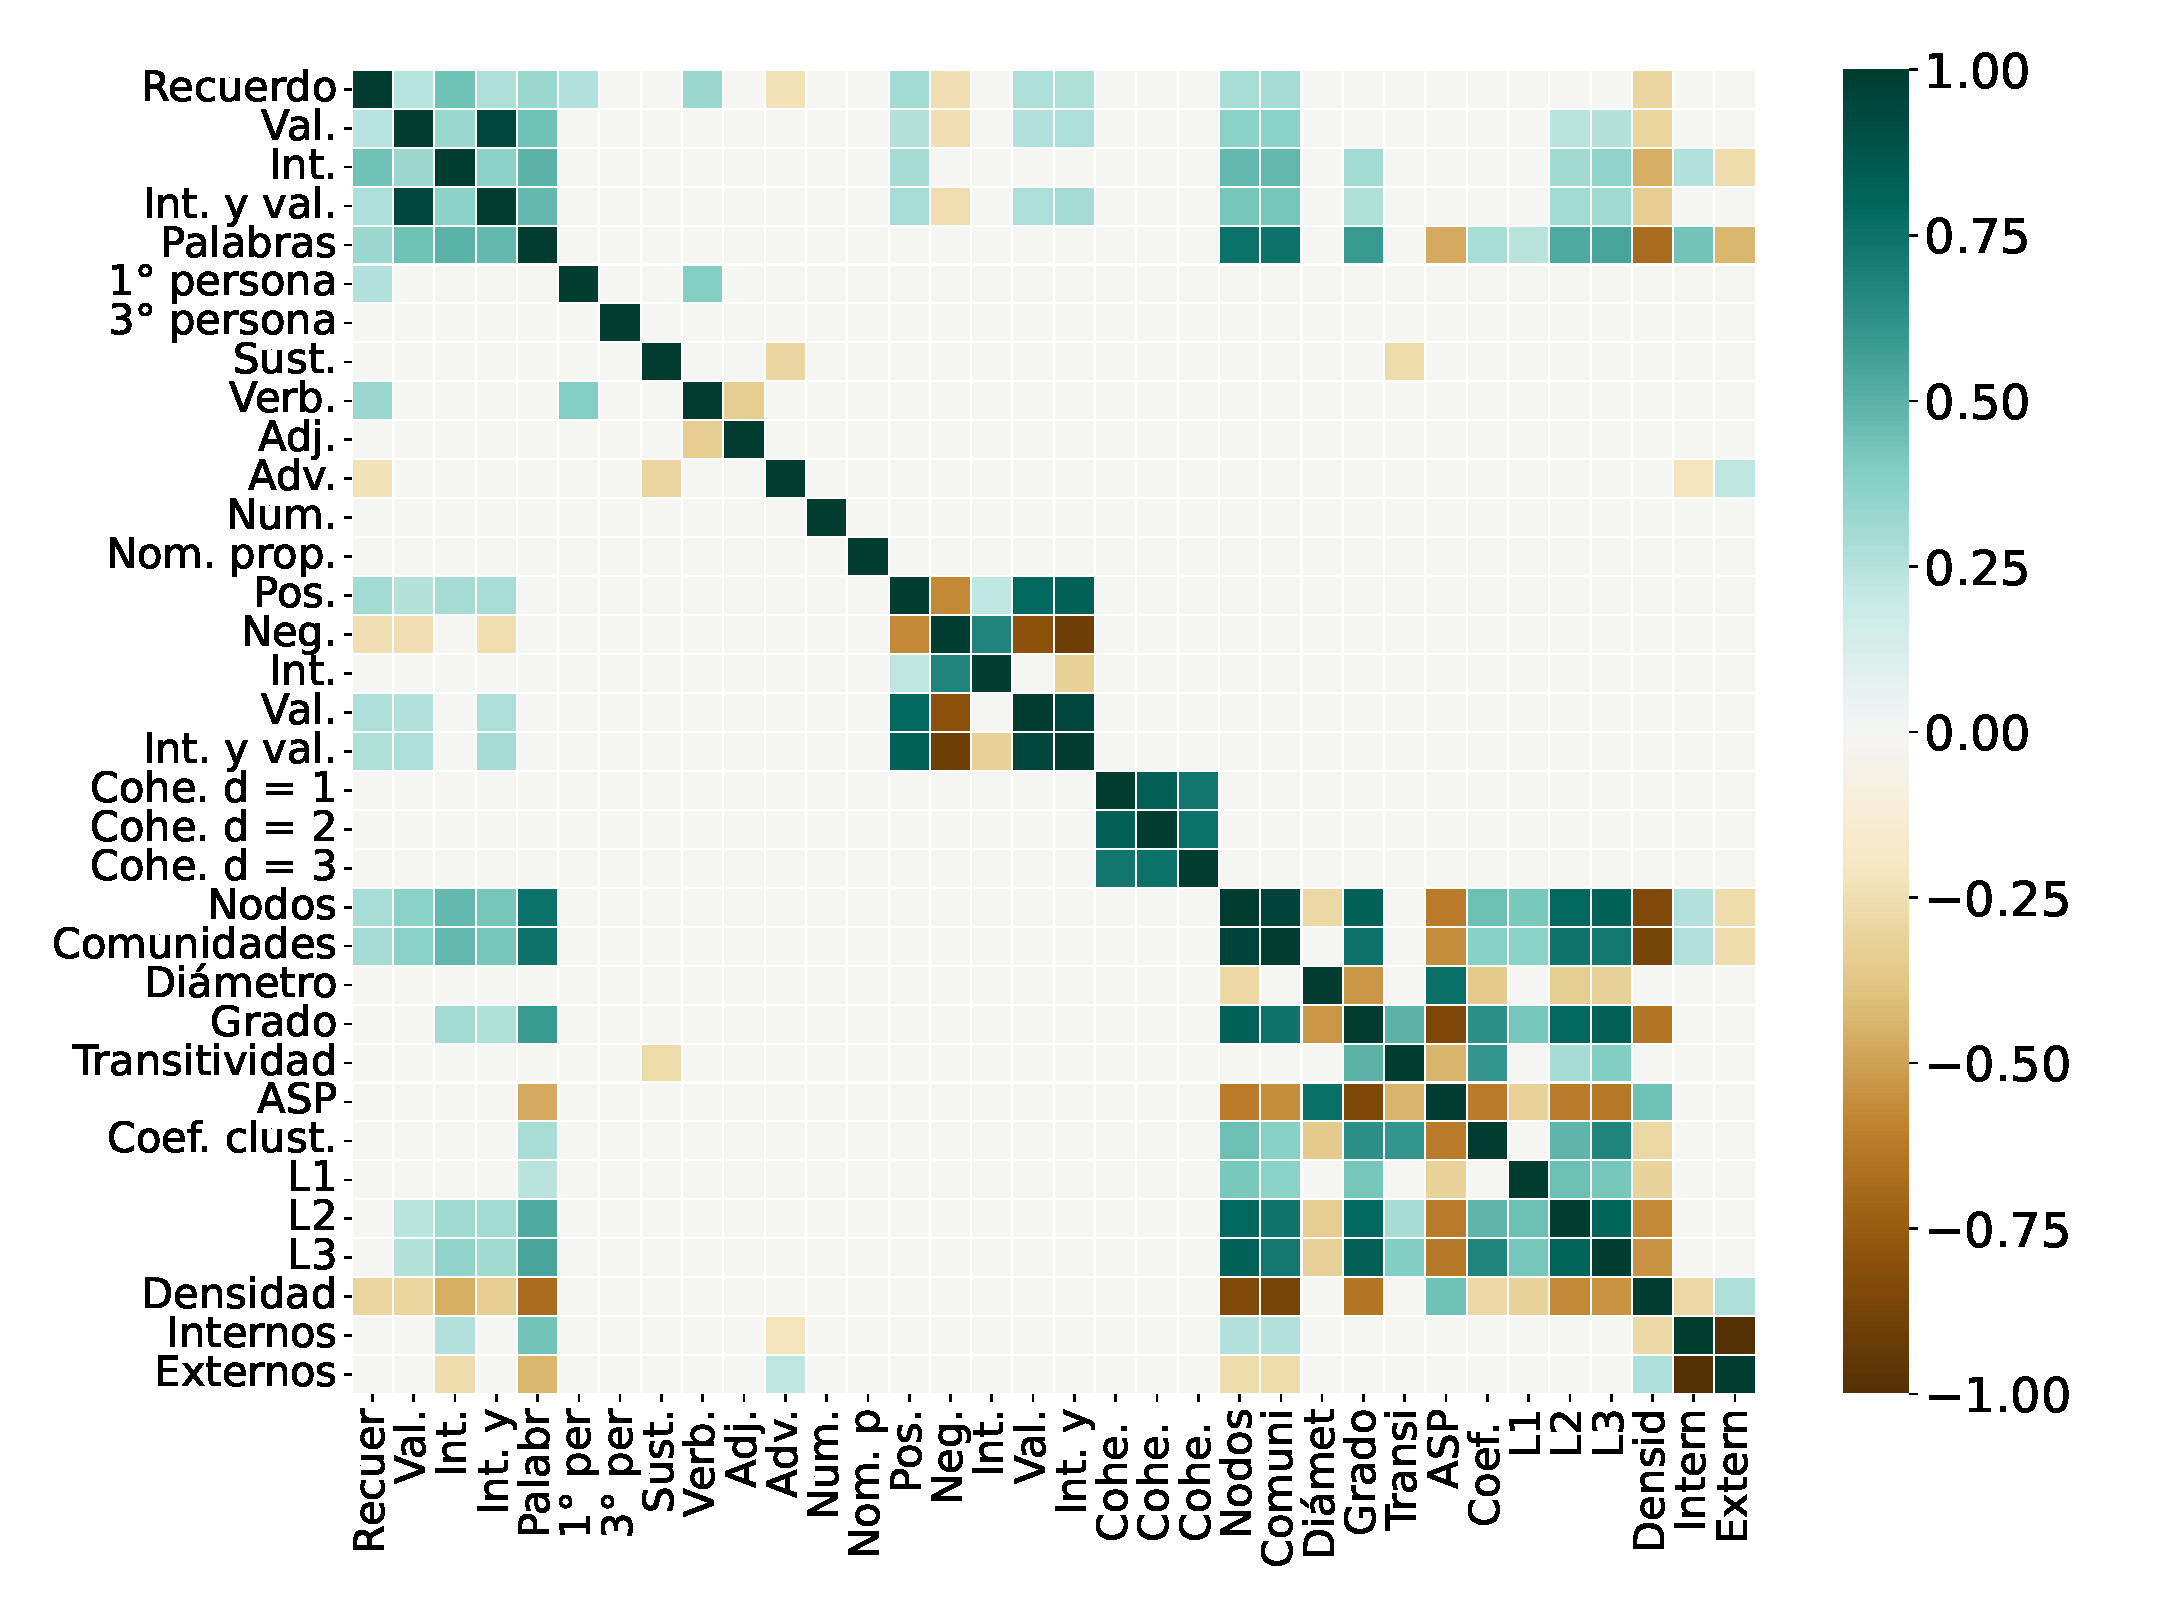
\includegraphics[width = 15cm]{figures/ch03/Correlacion/2correlacion_Primera.pdf} 
    \caption{Matriz de correlación de los cuantificadores de los relatos y las variables de autopercepción para la primer entrevista. Solo se presentan en color las correlaciones con un p$_{val}$ menor al significativo (9 $\times$ 10$^{-5}$ = 0,05/número de variables).}
\label{fig:cap3_corr}
\end{figure}

Se puede observar correlación entre todas las variables de autopercepción, y estas además correlacionan con el número de palabras. Es decir, cuando el número de palabras aumenta también lo hace el recuerdo valencia e intensidad autopercibida. Destaca además la correlación entre la valencia autopercibida con la calculada a través de pysentimiento y esto también sucede con la variable de intensidad y valencia. Con la variable de intensidad no se tuvo correlación.
El recuerdo autopercibido correlaciona con la variable positivo de pysentimiento, la valencia e intensidad y valencia, y anticorrelaciona con negativo. Es decir, los participantes dicen recordar mas los relatos clasificados como positivos y mas intensos, y menos los negativos y menos intensos. 
Además algunas variables de autopercepción correlacionan con algunas estructurales. Todas correlacionan con el número de nodos y comunidades en la componente fuertemente conexa que nos habla del largo del relato. Y también todas anticorrelacionan con la densidad, ... no se que decir de esto. Tampoco se que decir de las correlaciones con el grado y L2 Y L3...
Por último la intensidad autopercibida correlacionó con el número de detalles internos (episódicos) y anticorrelacionó con los externos (semánticos) lo cual es consistente con investigaciones previas (¿pongo citas en resultados?).
También correlaciona el recuerdo con primera persona verb y anticorr con adverbio, pero no se qué decir de eso, asi que mejor ni lo menciono, no?

A diferencia de las variables de autopercepción, no se tiene correlacion entre todas los variables de contenido. destaca que número de palabras correlaciona con varias medidas estructurales de las redes, y con las variables de memoria correlaciona con los detalles internos (episódicos), es decir, en los relatos en los que más se habla hay mas información episódica que semántica. También se ve una correlación entre el número de palabras en primera persona co enl número de verbos, y una correlación leve entre el número de adverbios y los detalles internos.

Observando las variables de sentimiento obtenidas del relato, estas correlacionan entre ellas, con excepción de intensidad y valencia que no correlacionan entre ellas. Destaca la leve correlación de los relatos positivos con la intensidad. Estas variables no correlacionan con ninguna otra variable obtenida de los relatos.

Las variables estructurales también tienen varias correlaciones entre ellas. Destaca que las variables de coherencia solo correlacionan entre ellas. Esta correlación es esperable pues los relatos mas coherentes entre oraciones contiguas siguen siendo los mas coherentes calculando cada dos oraciones o tres. Luego las variables de redes tienen varias correlaciones entre ellas, pero destaca la leve correlación del número de nodos y comunidades con el número de detalles internos (episódicos) y la anticorrelación con densidad. El número de nodos nos habla del tamaño de la red, por lo tanto es consistente esta correlación con la que se vió con el número de palabras.

Para finalizar, las variables de memoria anticorrelacionan entre ellas, esto se debe a que una es 1 - la otra (jaja ver como escribir).


Para el segundo tiempo se obtiene una matriz de correlación muy similar (ver Figura \ref{fig:cap3_corrsegt}). Destaca que ahora en las variables de autopercepción tampoco se observa correlación entre intensidad y valencia (cosa que ya sucedía con las variables calculadas por pysentimiento en el primer tiempo) y ahora el recuerdo autopercibido es el que correlaciona con los detalles internos. También destaca que los detalles internos correlacionan con el número de verbos. La verdad, no tengo mucho mas que decir, podría no ponerlo.



\begin{figure}[h]
    \centering
    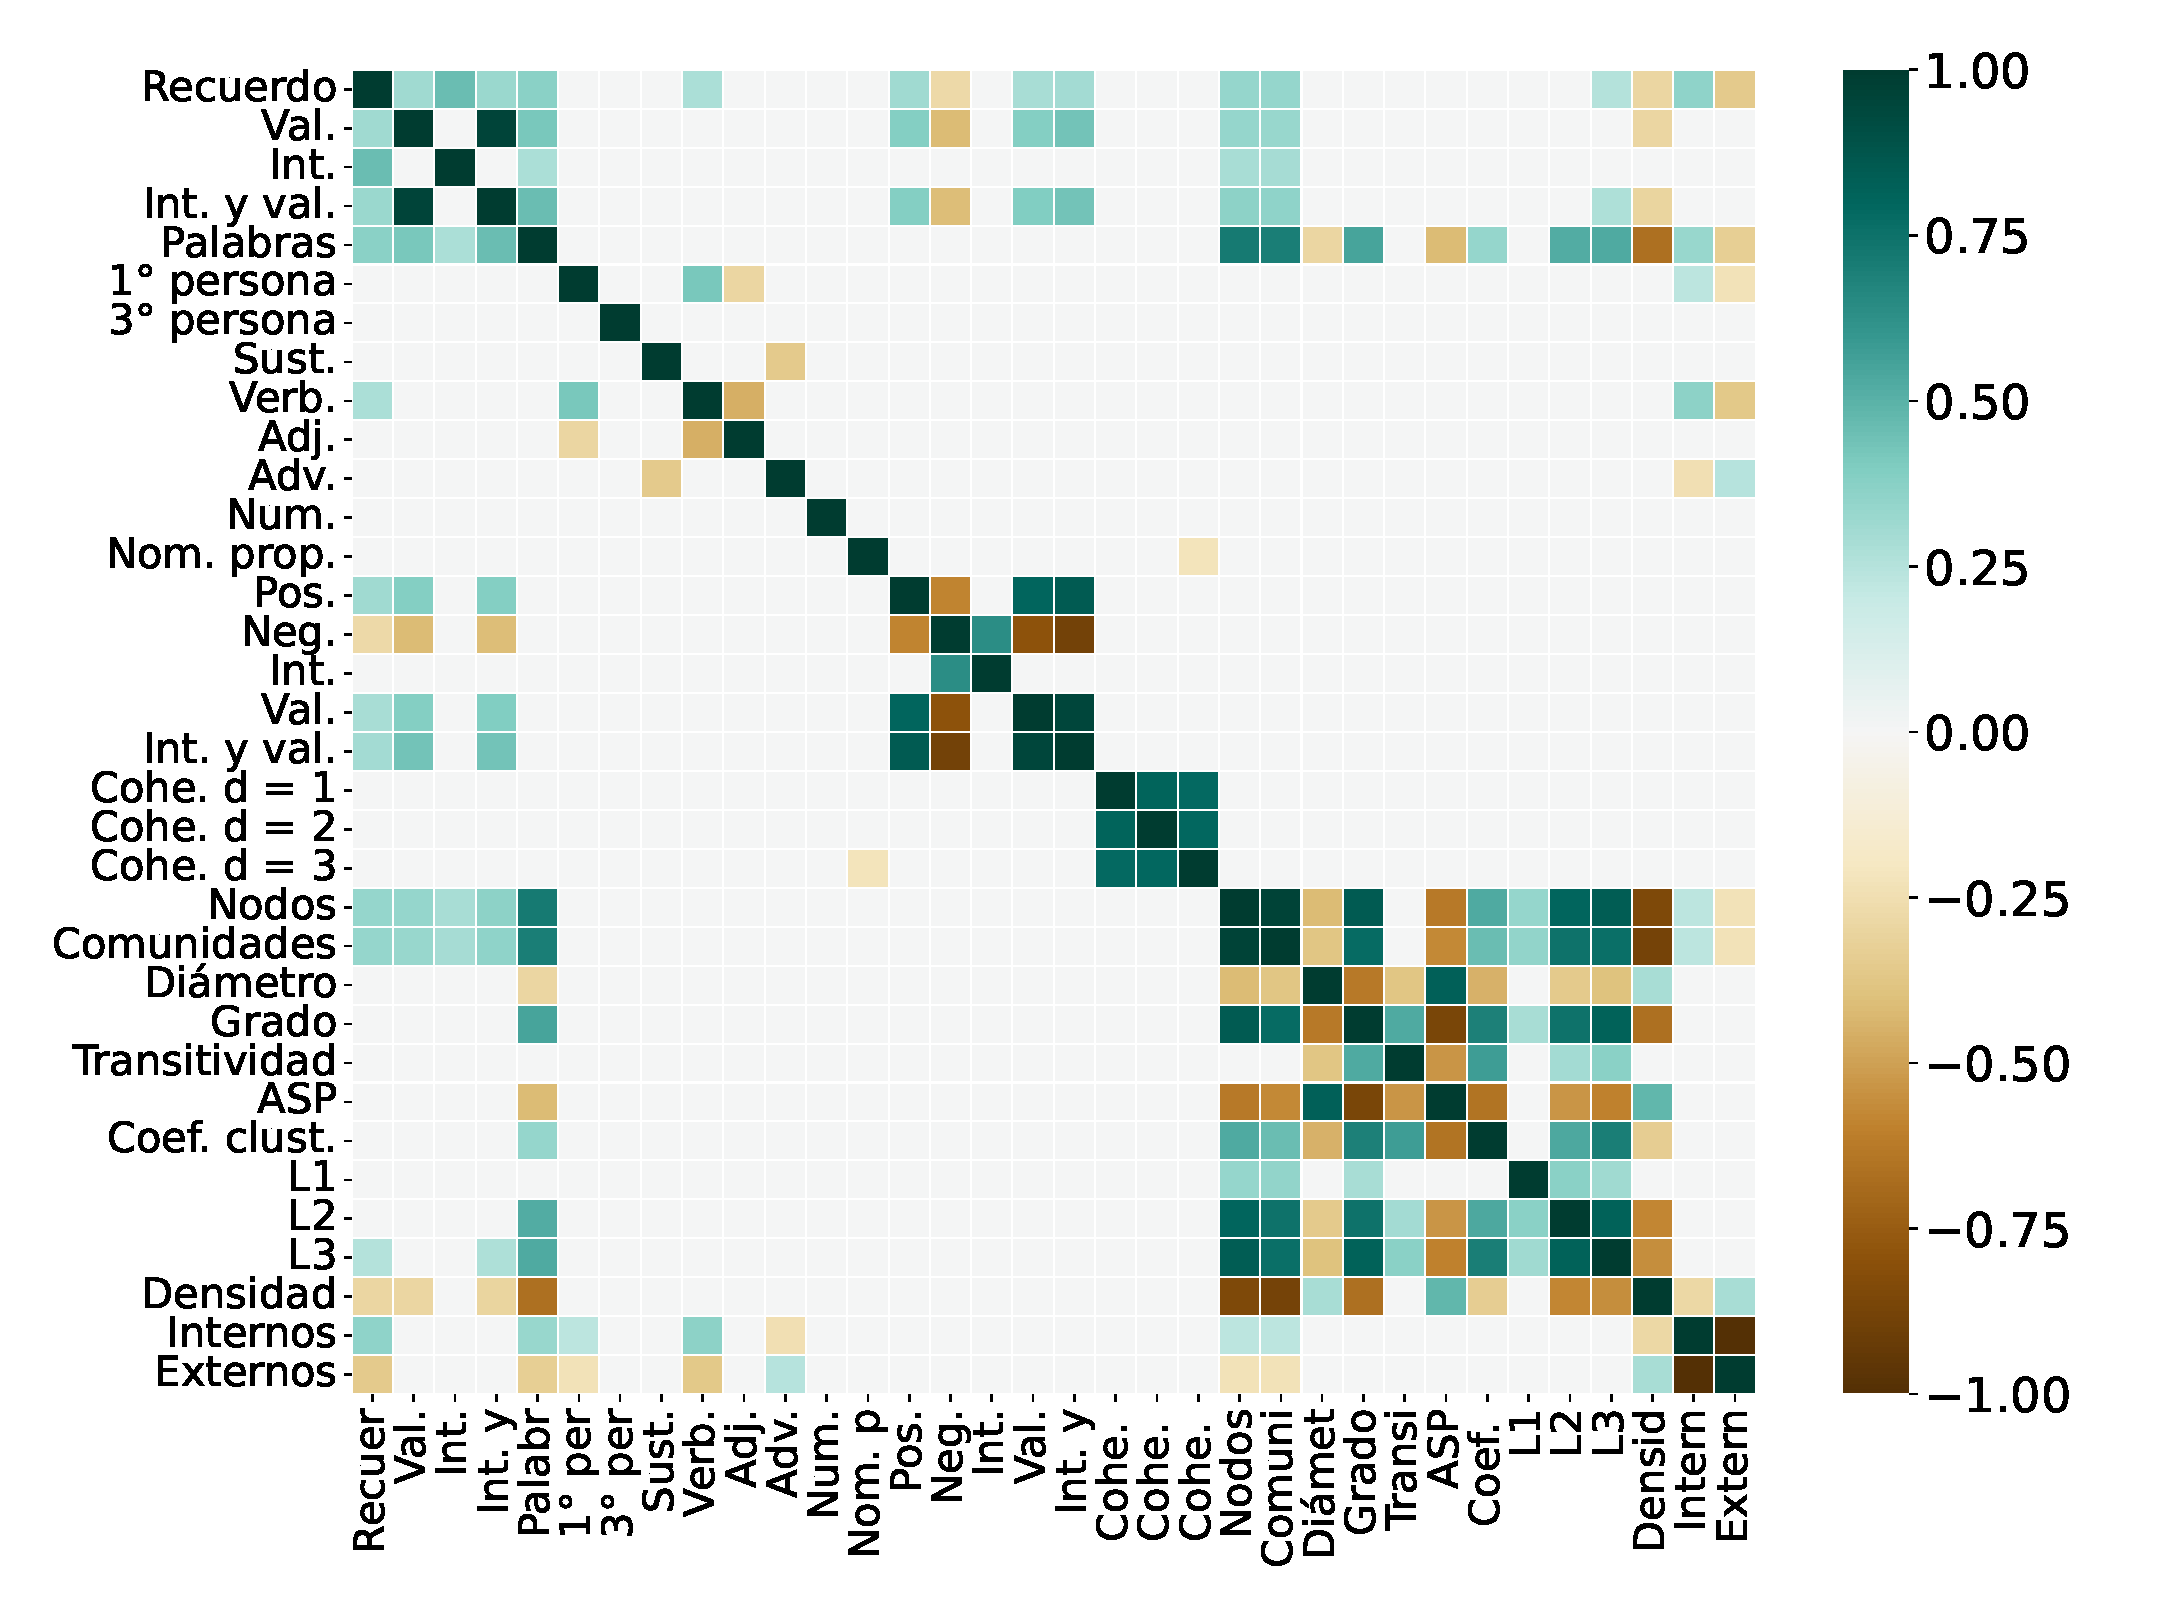
\includegraphics[width = 15cm]{figures/ch03/Correlacion/2correlacion_Segunda.pdf} 
    \caption{Matriz de correlación de los cuantificadores de los relatos y las variables de autopercepción para la segunda entrevista. Solo se presentan en color las correlaciones con un p$_{val}$ menor al significativo (9 $\times$ 10$^{-5}$ = 0,05/número de variables).}
\label{fig:cap3_corrsegt}
\end{figure}

\section{Busqueda de los cuantificadores usando PCA y aprendizaje no supervisado (o clustering)}

En esta sección se utilizará una reducción de dimensionalidad únicamente con las variables obtenidas de los relatos y luego se buscó el agrupamiento natural que surgía de los datos haciendo clustering con Kmeans.

El procedimiento fue el siguiente, inicialmente se buscó separar uno de los relatos autobiográficos, el relato de vuelta a la presencialidad del relato de control que era una memoria no consolidada (se le preguntaba a los participantes qué hicieron antes de ir a la entrevista). Se decidió utilizar estos dos relatos pues son los únicos dos que no son memorias colectivas y ponen prioridad a la primera persona. 
Inicialmente se buscaba el número óptimo de grupos con la validación interna dada por Silhouette. Para ello se hacía un análisis de componentes principales y se barría tanto el número de componentes como el número de grupos (clusters). Luego dejando fijo el número de grupos se hacía un barrido en el número de componentes principales y se volvía 
a hacer clustering con el objetivo de encontrar cuando se maximizaba la validación externa. La validación externa contaba de un test R que compara las etiquetas externas de los relatos con las obtenidas del agrupamiento con clustering. Luego, una vez que se tenía el número de componentes principales se buscaba las variables mas importantes en ellas. Estos resultados se pueden encontrar en la subsección \ref{sec:PCspresvscontrol}.

Se buscó las variables mas importantes de las componentes principales que optimizaban la validación externa para agrupar los relatos de presencialidad y control. Sólo con esas variables se seguía el mismo procedimiento para agrupar los relatos restantes (campeones, CFK y Arabia), lo cual se puede encontrar en la subsección \ref{sec:PCscamparCFK}.

\colorbox{yellow}{pongo esto aca no? Y en métodos solo explico el algoritmo de reducción usado y el de agrupamiento, no esto}

\colorbox{yellow}{en caso de mover esto a métodos, qué escribo aca para introducir?}


\subsection{Memoria autobiográfica contra memoria no consolidada}
\label{sec:PCspresvscontrol}

Se buscó el agrupamiento natural que surgía al hacer clustering en los relatos de presencial y control luego de aplicar una reducción de dimensionalidad.
Inicialmente se buscó con la validación interna de Silhouette cuál era el número de grupos óptimo para la separación. Dado a que también se iba a hacer una redución de dimensionalidad con PCA se hizo un barrido no sólo en el número de grupos, sino también en el número de componentes principales, y en cada caso se buscó el coeficiente promedio de Silhouette. Estos resultados se pueden ver en la Figura \ref{fig:cap3_defk_controlpres}(a). Se puede observar que en todos los números de componentes principales el mayor coeficiente de Silhouette promedio corresponde a dos clusters, cuyo perfil de Silhouette para el caso de 9 componentes principales se puede observar en la Figura \ref{fig:cap3_defk_controlpres}(b). En la misma se puede apreciar que todos los elementos del primer cluster se encuentran con un coeficiente positivo, mientras que en el segundo cluster menos del 10$\%$ tienen un coeficiente negativo. Se decidió continuar entonces con dos grupos. \colorbox{yellow}{decidí mostrar con 9PCs pq después es lo que usamos, pero en 6 PCs no da negativo nada, muestro mejor ese?}

\begin{figure}[h]
    \centering
    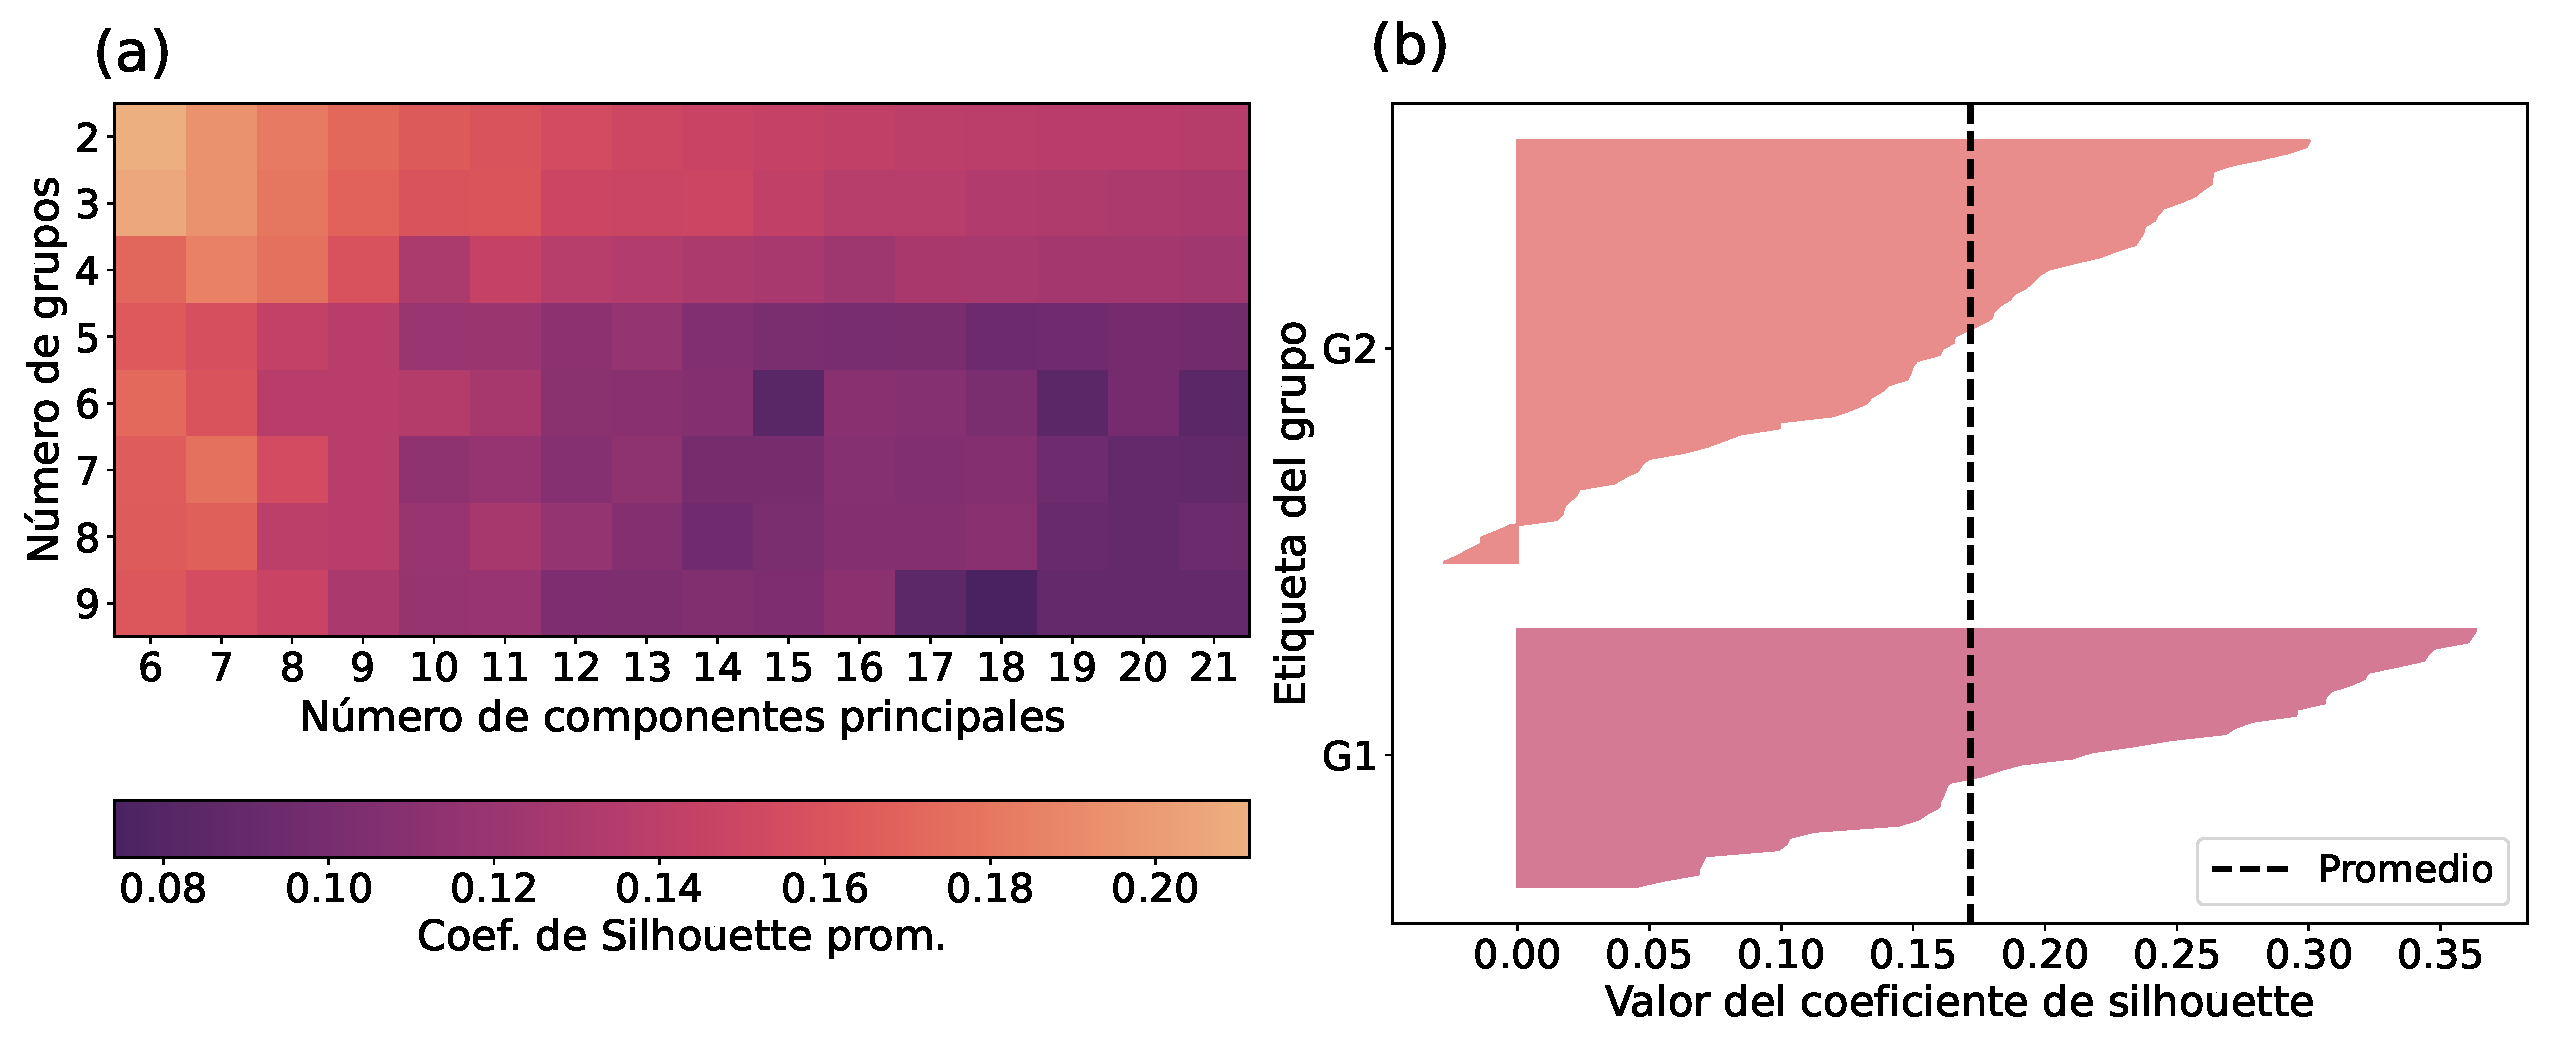
\includegraphics[width = 15cm]{figures/ch03/PCA_clustering/Primer tiempo/silhouette2_pres_control_perfil9PCs.pdf} 
    \caption{Gráficos para la definición del número de clusters utilizado para el agrupamiento de los relatos de presencial y control. En \textbf{(a)} se observa la matriz del coeficiente de Silhouette promedio en un barrido del número de clusters y el número de componentes principales utilizadas. El valor del coeficiente viene dado por la barra de color debajo de la matriz. Se graficó de 6 a 21 componentes principales pero en todo el rango se veía el mismo comportamiento. En \textbf{(b)} se observa el perfil de Silhouette para dos clusters cuando se toman 9 componentes principales.}
\label{fig:cap3_defk_controlpres}
\end{figure}

Luego se buscó el número de componentes principales que maximizan la validación interna hecha con el índice R. Para ello se graficó este índice en función del número de componentes como se ve en la Figura \ref{fig:cap3_defpcscontrolpres}(a). En esta se observa que el índice R toma su máximo valor desde las 9 componentes principales en adelante. Con la intención de reducir la dimensionalidad se decidió tomar solo 9 componentes principales. La varianza total acumulada en estas componentes es de casi el 80$\%$ como se puede observar en la Figura \ref{fig:cap3_defpcscontrolpres}(b).

\begin{figure}[H]
    \centering
    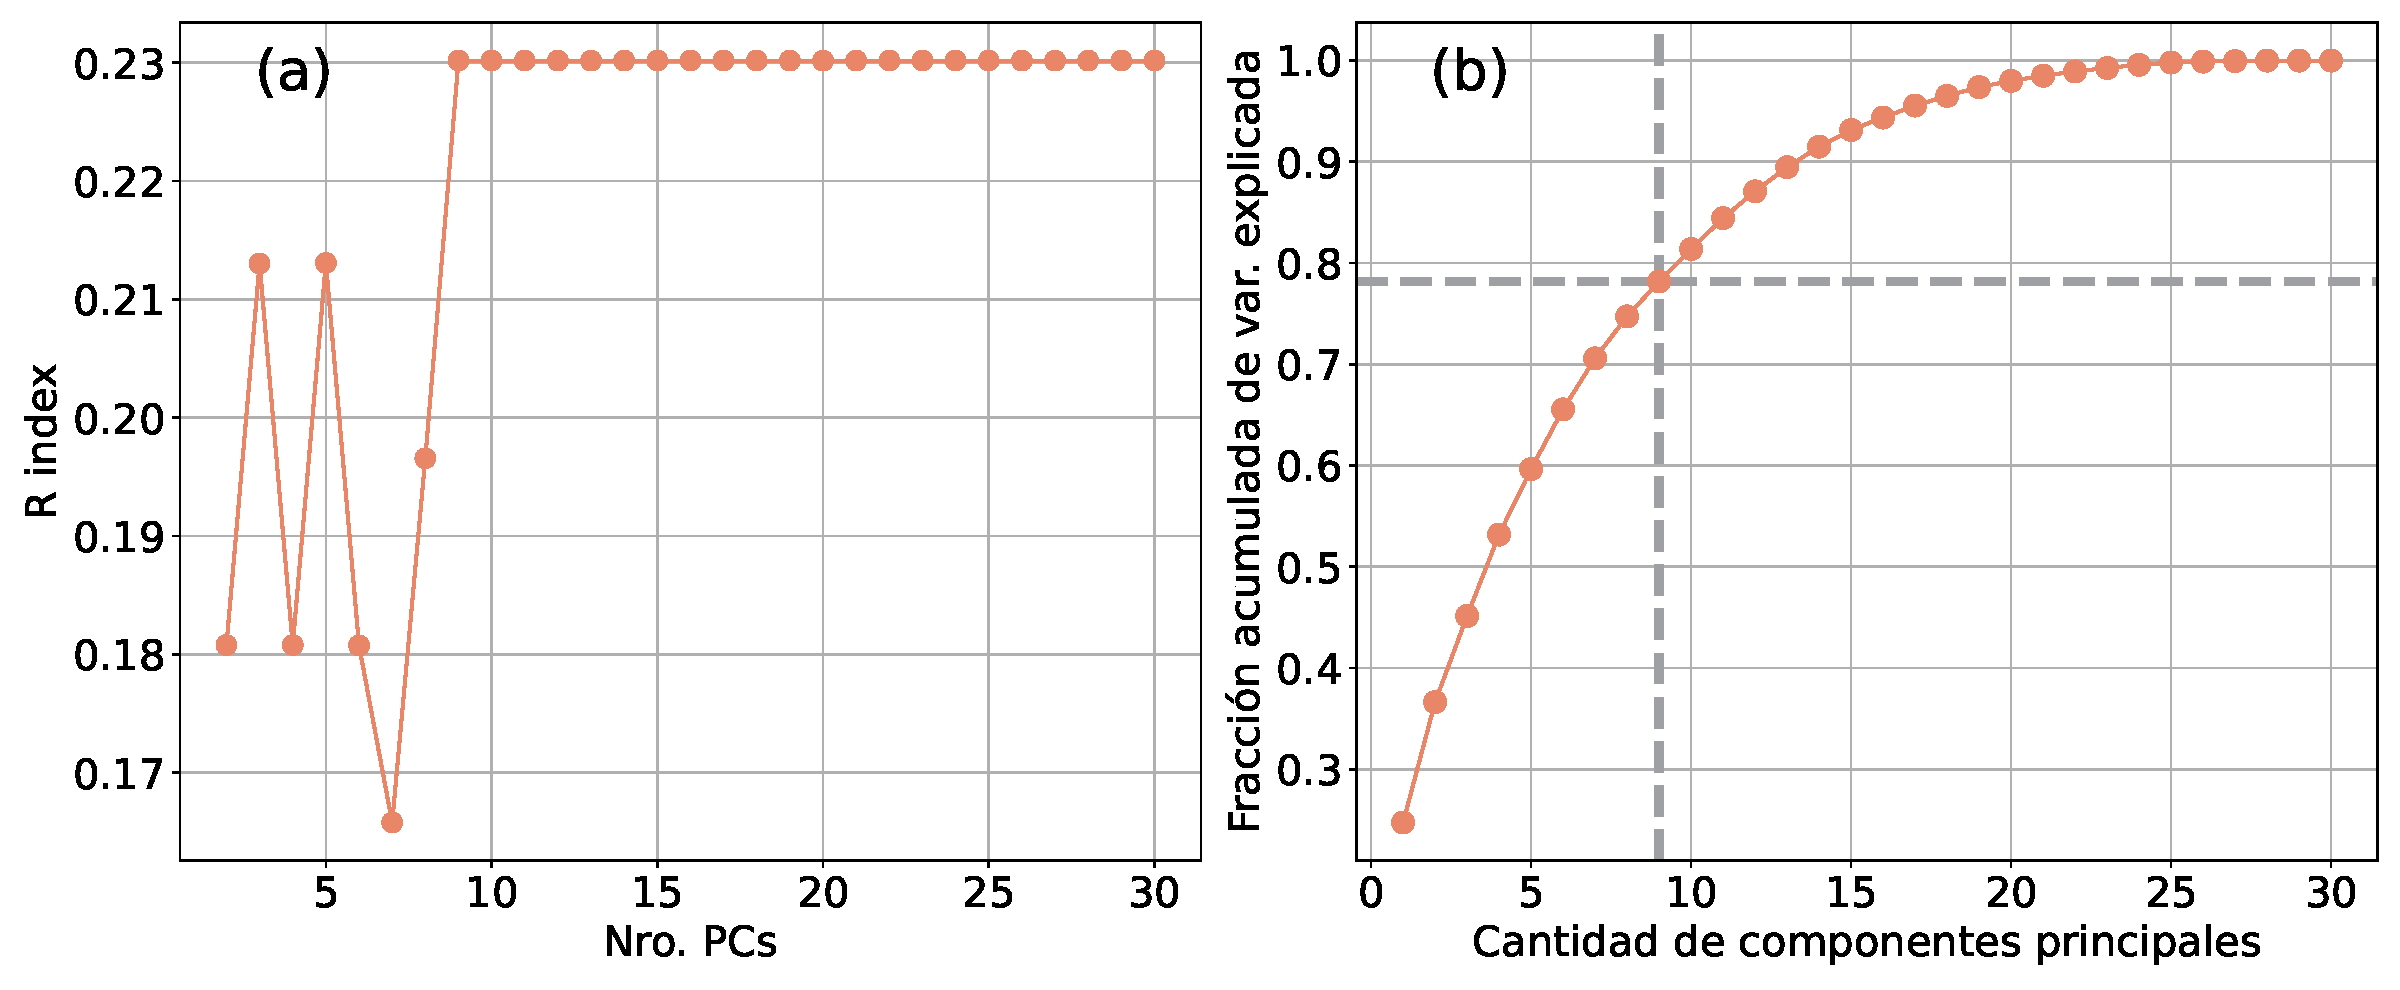
\includegraphics[width = 15cm]{figures/ch03/PCA_clustering/Primer tiempo/RindexyPCs_pres_control.pdf} 
    \caption{Definición número de componentes principales. En \textbf{(a)} se observa el índice R en función del número de componentes principales. En \textbf{(b)} la varianza total acumulada al aplicar el análisis de componentes principales. Se marca en línea punteada el valor que toma para 9 componentes.}
\label{fig:cap3_defpcscontrolpres}
\end{figure}

En la Figura \ref{fig:cap3_9PCscontrolpres} se graficó la dependencia de las componentes principales en función de las variables originales. Destaca que la mayoría de componentes principales son principalmente combinaciones lineales de variables de la misma categoría. Se puede observar que la primer componente principal depende principalmente del número de palabras y la mayoría de variables estructurales de redes. En la segunda componente tienen mucho peso todas las variables de sentimiento menos intensidad. La tercer componente tiene principalmente variables estructurales de coherencia, aunque también tienen importancia no despreciable variables de contenido y memoria, al igual que la cuarta componente donde la importancia de cada categoría se ve mas distribuida. La quinta componente principal tiene principalmente variables de memoria. La sexta, octava y novena son variables de contenido, y la séptima mezcla variables de contenido y sentimiento.

\colorbox{yellow}{no se si no mover esto a apéndice}

\begin{figure}[h]
    \centering
    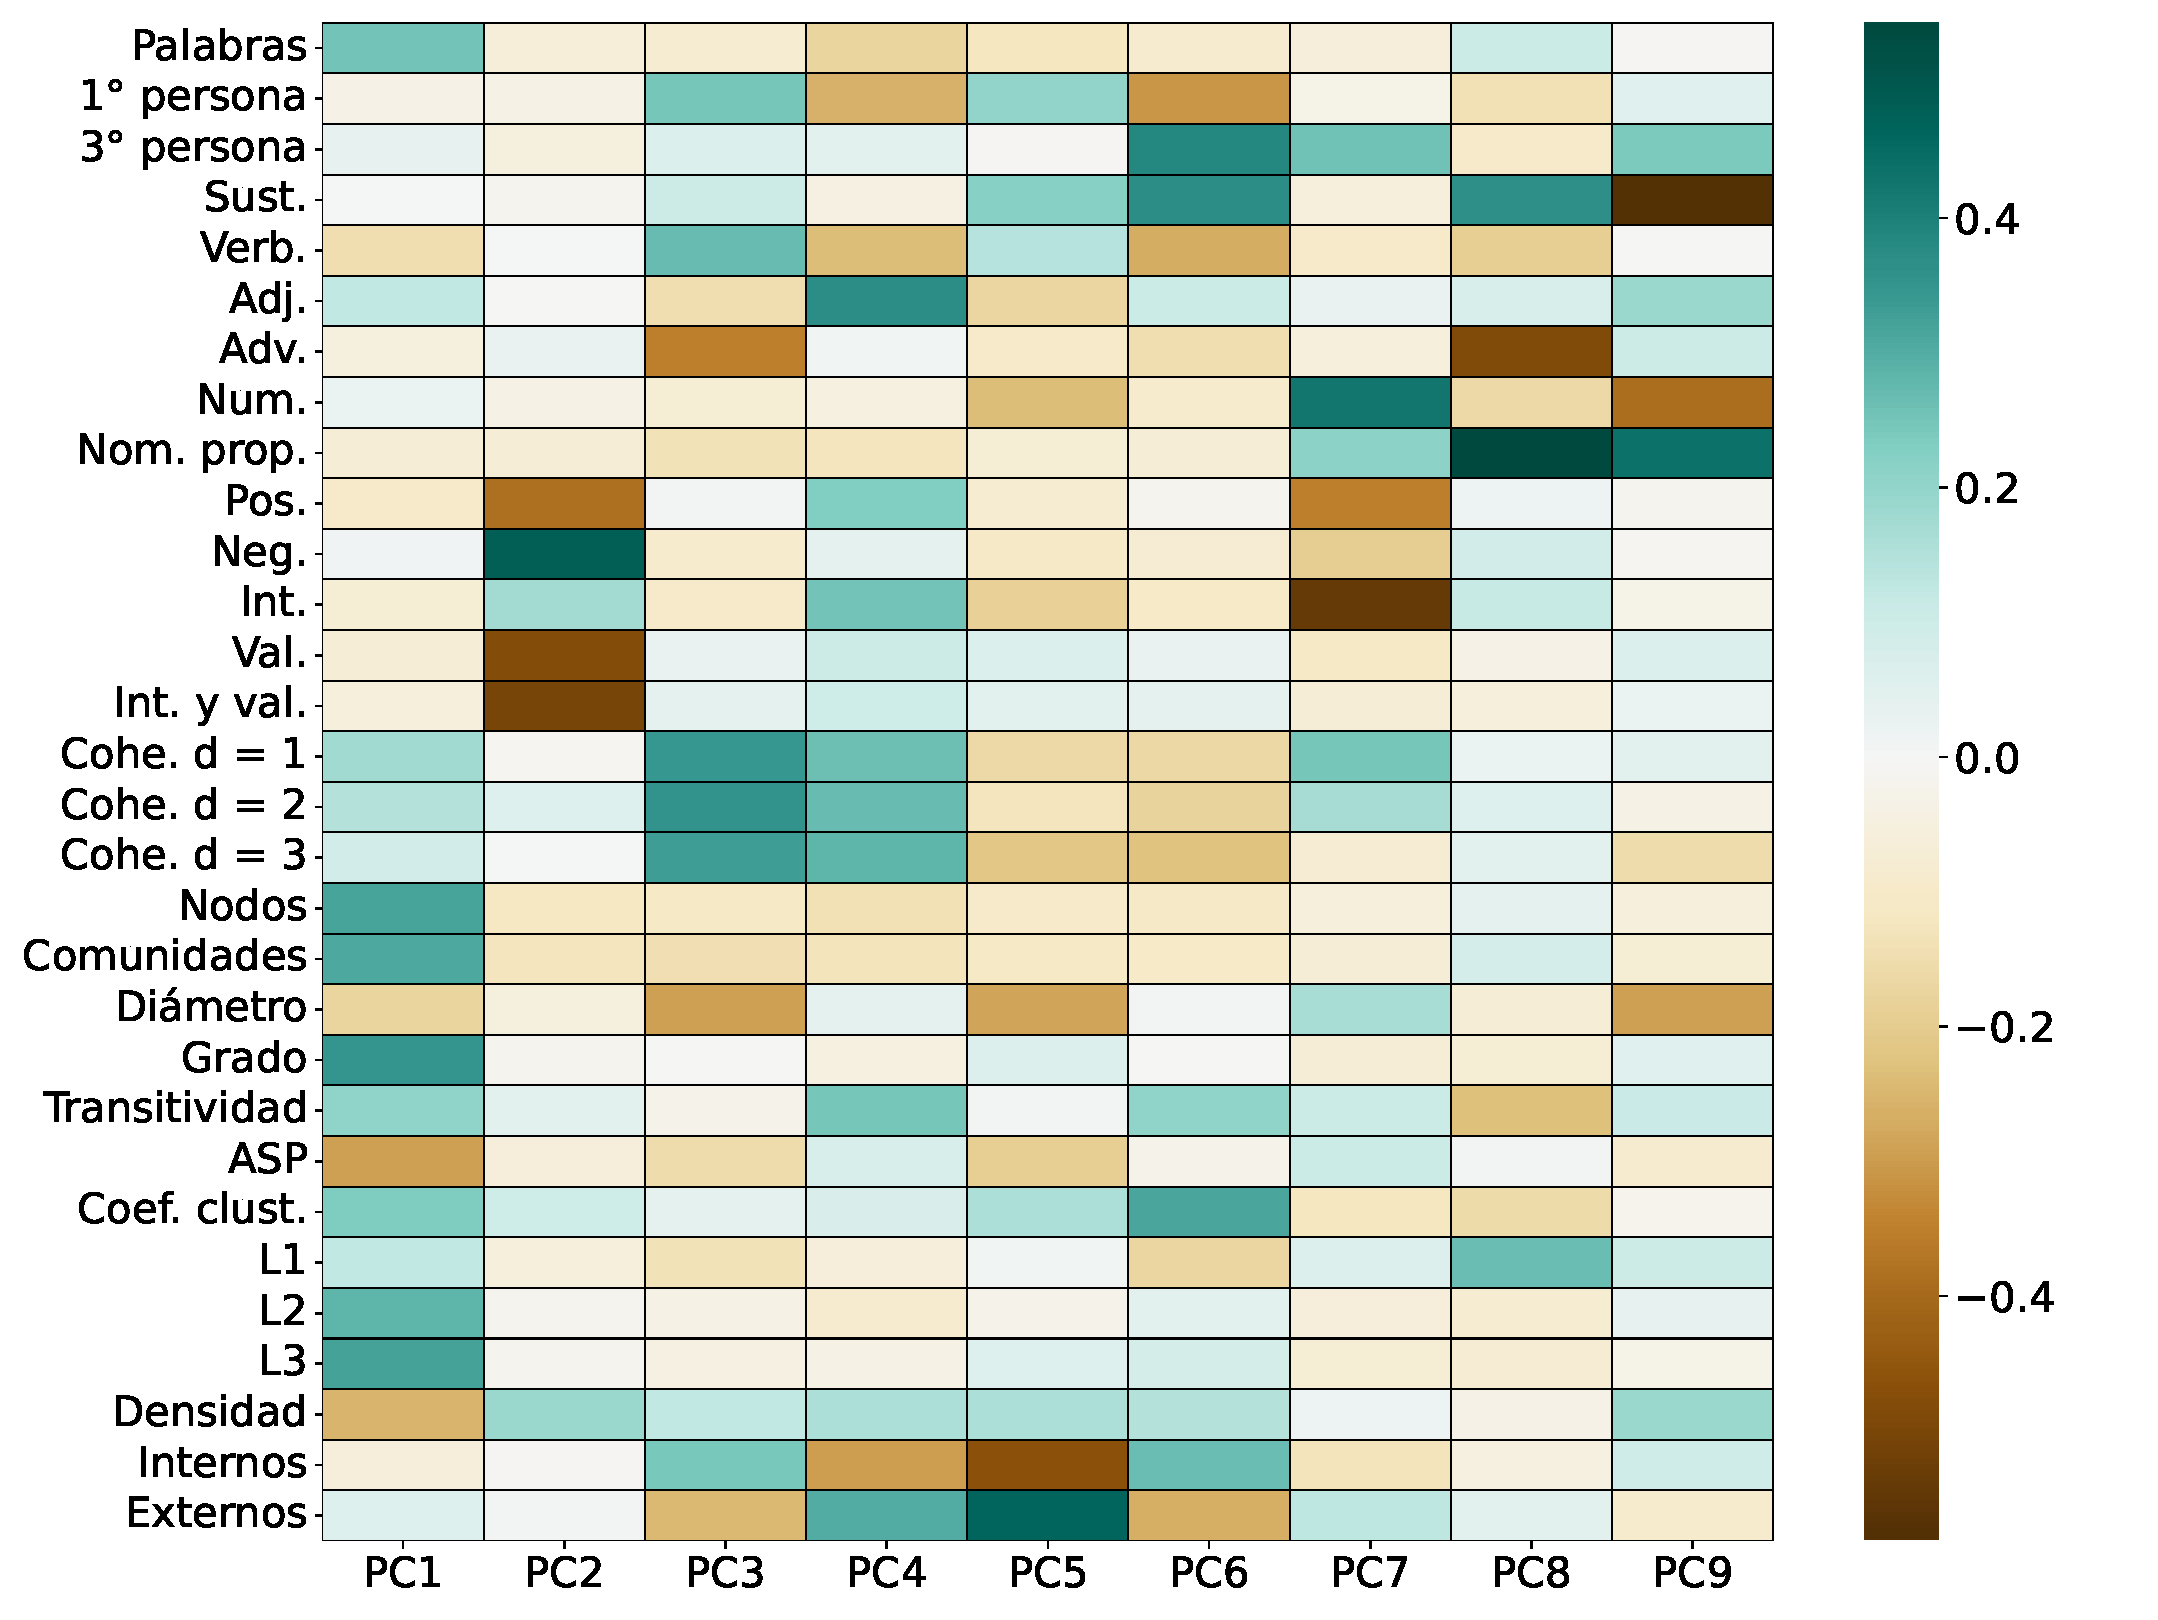
\includegraphics[width = 15cm]{figures/ch03/PCA_clustering/Primer tiempo/9PCs_pres_control.pdf} 
    \caption{Combinación lineal de las componentes principales de los relatos de presencial control en función de las variables originales. El color indica el coeficiente que acompaña a la variable en la combinación lineal.}
\label{fig:cap3_9PCscontrolpres}
\end{figure}

Finalmente se graficó los datos de los relatos de presencial y control en la primera y segunda componente principal como se puede observar en la Figura \ref{fig:cap3_PC1vsPC2presycontrol}. En la misma el color representa los distintos relatos y la forma los distintos grupos. El índice R es de 0,23 y la matriz de confusión se puede observar en la Tabla \ref{tab:confusion_matrix_PyC}.

\begin{table}[htbp]
    \centering
    \begin{tabular}{|l|c|c|c|}
        \hline
        \multicolumn{1}{|c|}{} & \multicolumn{3}{c|}{\textbf{Condición real}} \\
        \cline{2-4}
        \multicolumn{1}{|c|}{} & & \textbf{Control} & \textbf{Presencial} \\
        \hline
        \multirow{2}{*}{\textbf{Condición clustering}} & \textbf{Control} & 47 & 18 \\
        \cline{2-4}
        & \textbf{Presencial} & 10 & 36 \\
        \hline
    \end{tabular}
    \caption{Matriz de confusión para las condiciones de presencial y control.}
    \label{tab:confusion_matrix_PyC}
\end{table}


\begin{figure}[h]
    \centering
    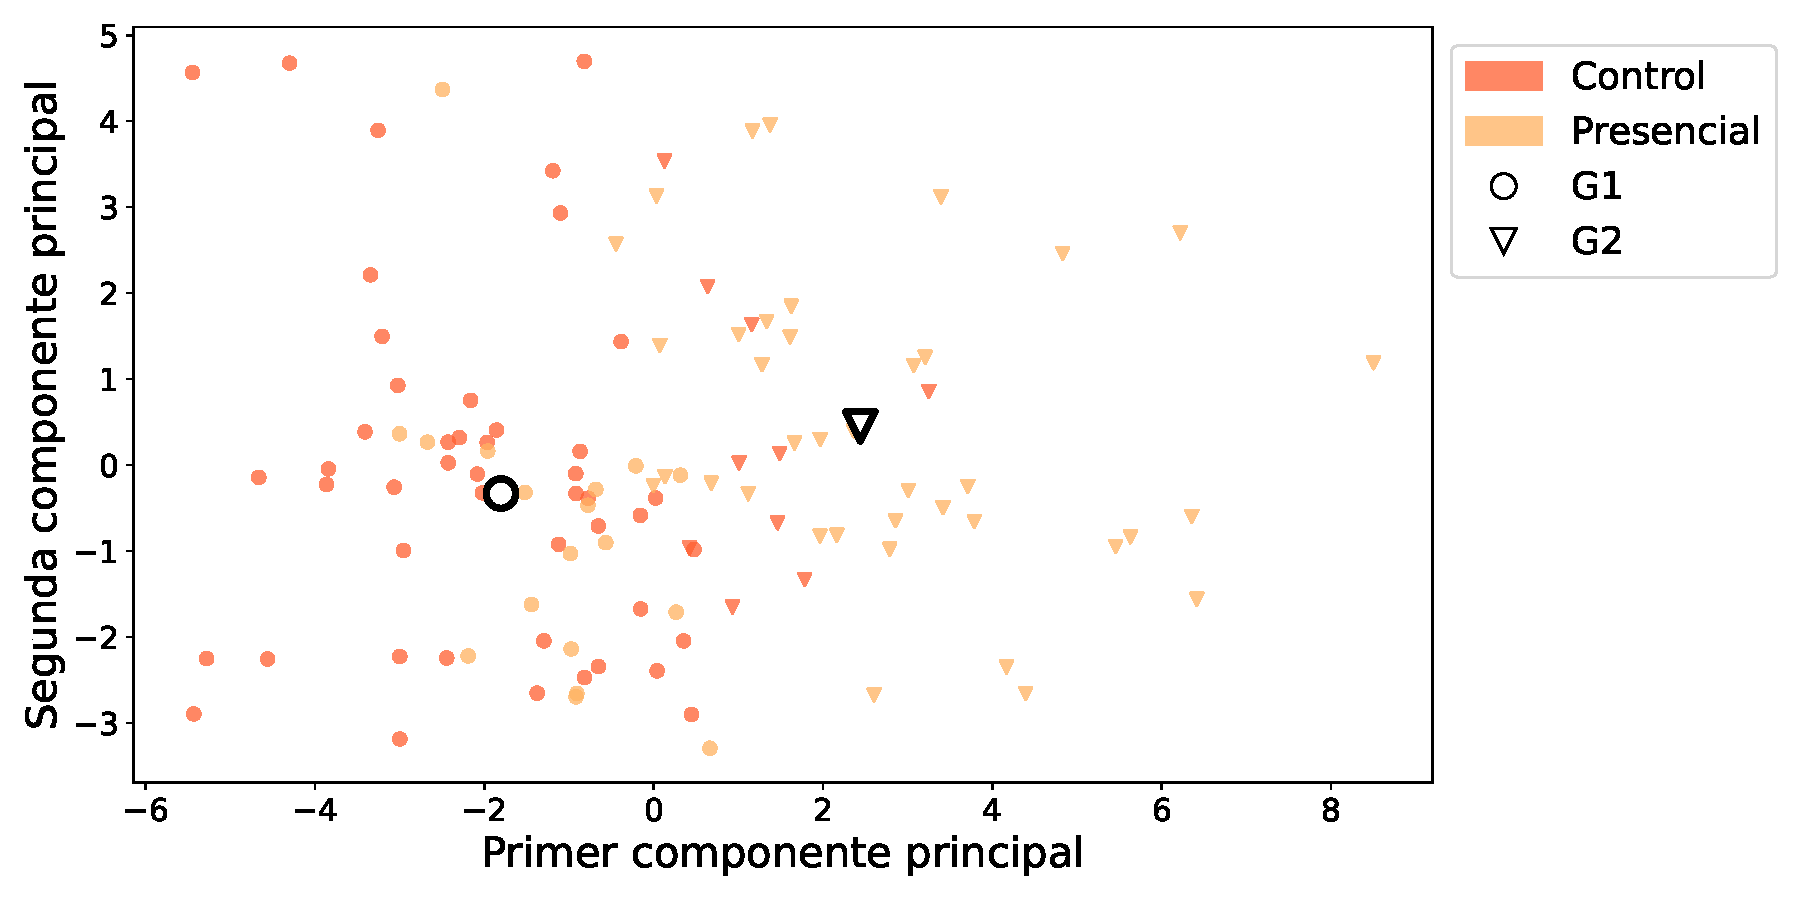
\includegraphics[width = 15cm]{figures/ch03/PCA_clustering/Primer tiempo/presvscontrol_NOenespaciocosine_PC1vsPC2_markersclusters_colortemas.pdf} 
    \caption{Resultado del clustering para las condiciones de control y presencial. El color representa las distintas condiciones, las formas los distintos grupos (clusters). El índice R es de 0,23.}
\label{fig:cap3_PC1vsPC2presycontrol}
\end{figure}


\subsection{Memorias con distinta valencia e intensidad}
\label{sec:PCscamparCFK}

Se continuó buscando agrupar las condiciones de CFK, Arabia y campeones.  Inicialmente se buscó el número de grupos óptimo para agrupar mediante una validación interna con el coeficiente de Silhouette. Para ello se calculó el coeficiente de Silhouette promedio haciendo un barrito tanto en el número de grupos y el número de componentes principales. Los resultados se pueden observar en la Figura \ref{fig:cap3_defk_cfkArCamp}(a) donde se puede ver que para todas las componentes principales se obtiene el mayor coeficiente de Silhouette promedio con 2 grupos. En la Figura \ref{fig:cap3_defk_cfkArCamp}(b) se puede observar el perfil de Silhouette en el caso particular de usar solo dos componentes principales, se puede ver que en el primer grupo todos los elementos fueron clasificados con coeficientes de Silhouette mayor a 0 y en el segundo grupo menos del 3$\%$ fue clasificado con un coeficiente menor a 0. Dado a que los relatos son de tres condiciones distintas se investigó cómo se distribuyen los relatos entre los grupos. Se observó lo que suele suceder es que se tiene un grupo del relato de campeones y otro de los relatos de CFK y Arabia. Si se aumenta el número de grupos el cluster de campeones sigue unido mientras que el otro se va dividiendo mezclando ambos relatos. Estos resultados se pueden ver en el Apéndice \colorbox{yellow}{hacer. o lo discuto después de la última figura de pc1 vs pc2 aumentando el número de grupo?}

\colorbox{yellow}{discutir en discusión que debe ser por la valencia e intensidad q no son muy distintas}. Se decidió continuar entonces tomando solo dos grupos.

\begin{figure}[h]
    \centering
    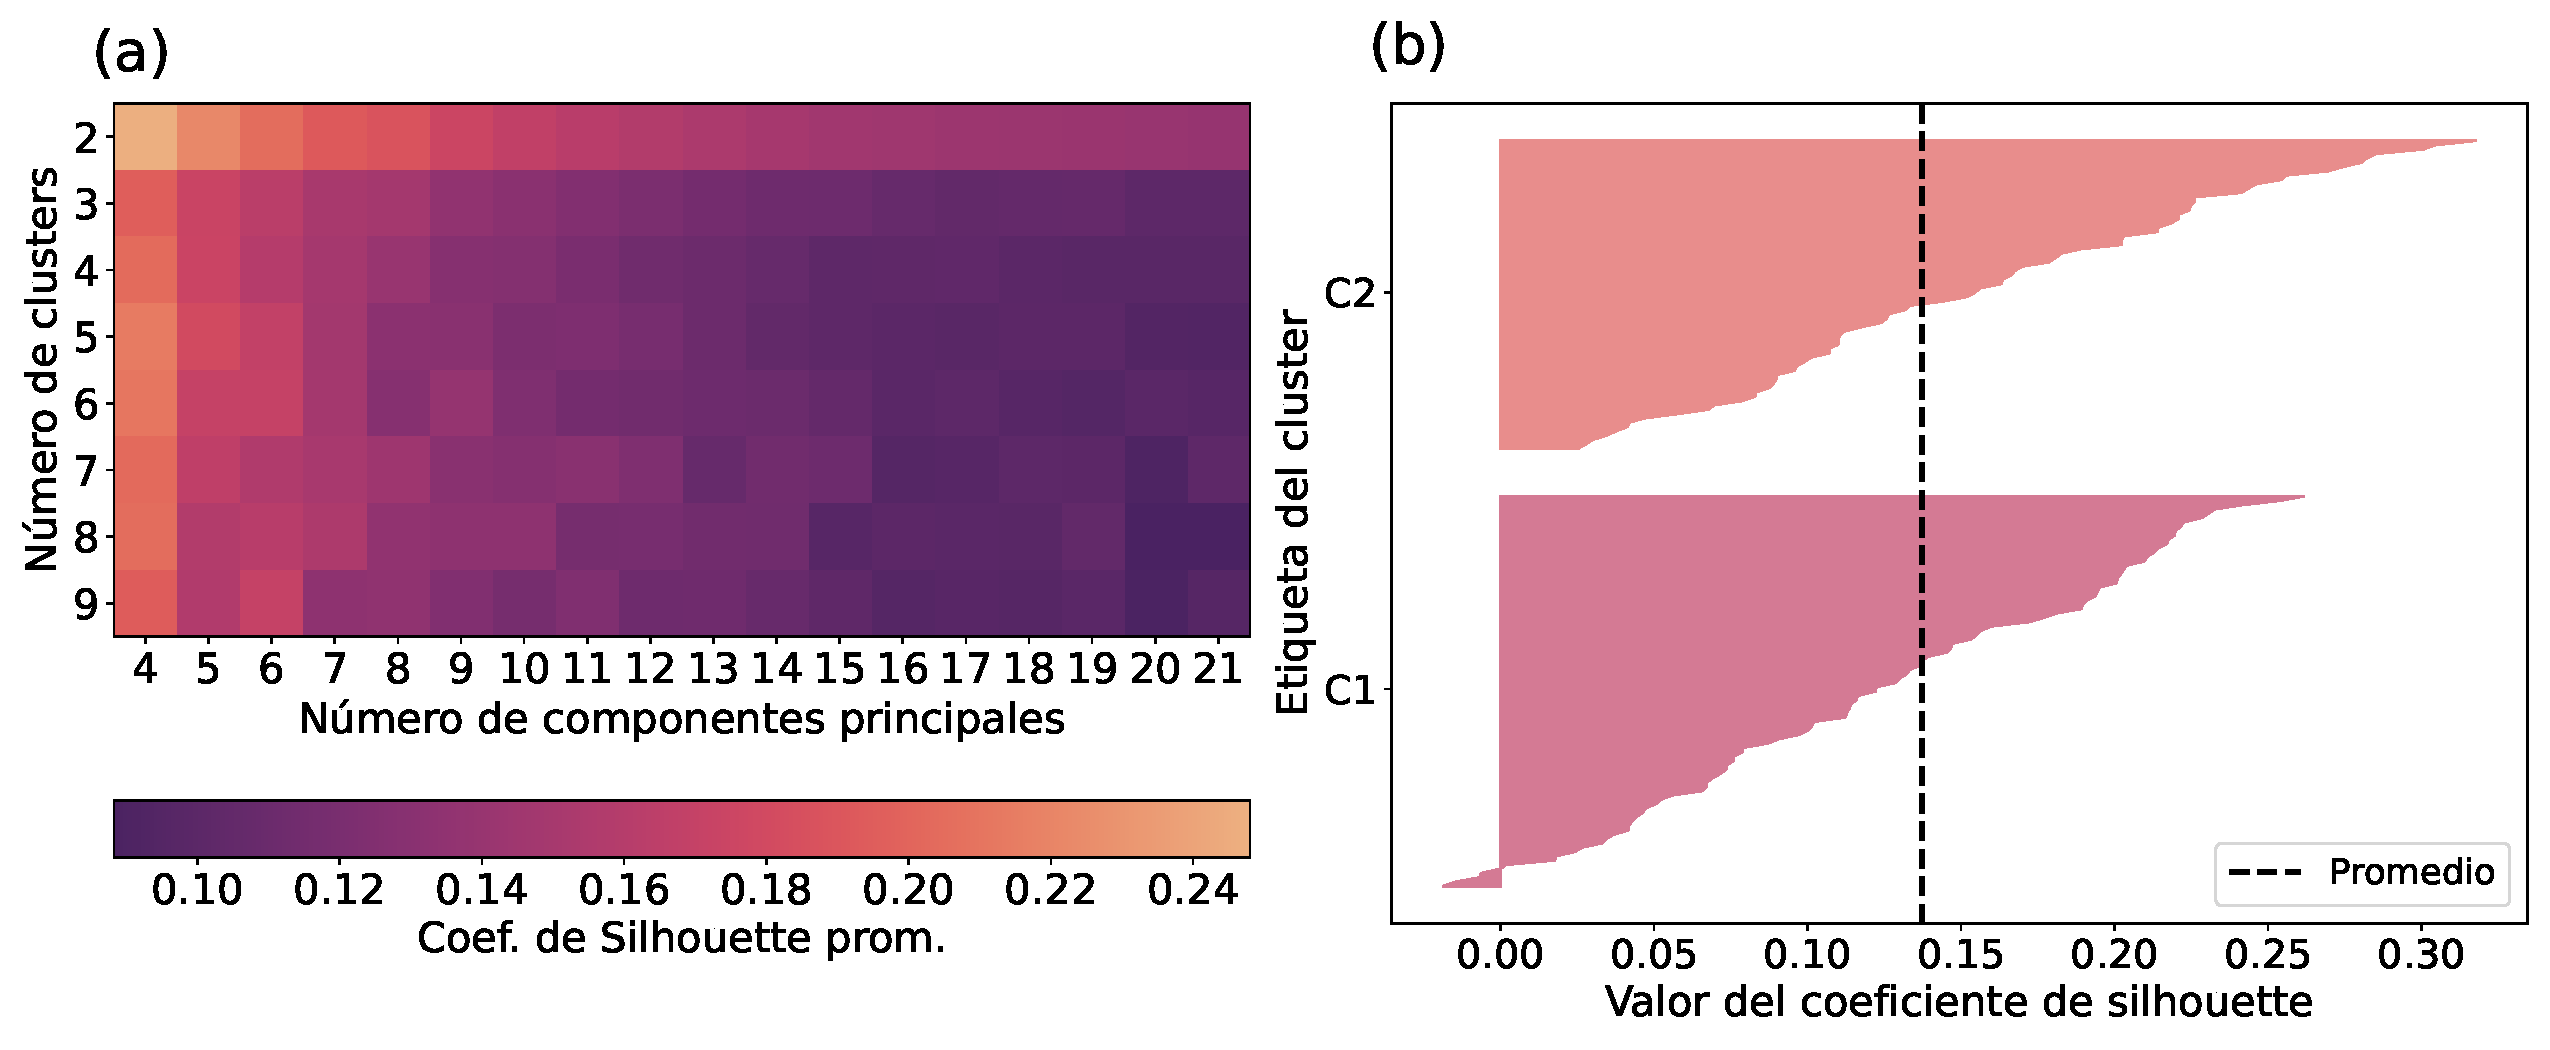
\includegraphics[width = 15cm]{figures/ch03/PCA_clustering/Primer tiempo/silhouette2_cfk_pres_ar_control.pdf} 
    \caption{Definición del número de grupos mediante validación interna con el coeficiente de Silhouette. En \textbf{(a)} se observa el coeficiente de Silhouette promedio de los relatos CFK, Arabia y campeones al hacer un barrido del número de grupos y el número de componentes principales. El barrido de número de componentes se hizo para todo el rango posible pero no se graficó todo por cuestiones de visualización. En todo el rango el comportamiento es similar. En \textbf{(b)} se observa el perfil de Silhouette para el caso particular de dos componentes principales.}
\label{fig:cap3_defk_cfkArCamp}
\end{figure}

Luego se buscó el número óptimo de componentes principales y las variables a utilizar para hacer el agrupamiento.\colorbox{yellow}{de aca} Para seleccionar las variables se tomó las 9 componentes principales utilizadas en la separación de los relatos de presencial y control (de la Figura \ref{fig:cap3_9PCscontrolpres}) y se buscó las variables mas importantes en estas. El barrido fue hecho de la siguiente manera, inicialmente se tomaban n variables de la primer componente principal, donde en caso de que n no sea un número entero se lo redondeaba. Luego para elegir cuántas variables se tomaba de la segunda componente se buscaba cuánta varianza explicaba la misma, llamamosle a esta cantidad $var_{PC2}$, y se la comparaba respecto de la varianza de la primer componente principal $var_{PC1}$. Luego, se tomaban n$\frac{var_{PC2}}{var_{PC1}}$ variables de la segunda componente principal. En caso de no ser un número entero se lo redondeaba. Para la tercera se n$\frac{var_{PC3}}{var_{PC1}}$ tomaban variables, y así se hizo con cada componente. Luego se utilizaba la unión de todas estas variables para hacer el agrupamieto.\colorbox{yellow}{hasta aca podría ir en métodos}. 
Entonces se hizo un barrido del número de componentes pricipales y el número de variables que se tomaba de la primer componente principal y se hacía reducción de dimensionalidad y después clustering de los relatos de CFK, Arabia y campeones, y para cada combinación se calculaba el índice R para hallar la combinación que maximizaba esta validación externa. En la Figura \ref{fig:cap3_defPCs_cfkArCamp}(a) se observan estos resultados. Se obtiene que el mayor índice R eliminando siete variables (primera persona, número de verbos, coherencia a distancia 3, diámetro, transitividad, coeficiente de clustering promedio y loops de uno). El número de componentes principales puede ser 2, 3 o 4, en todos esos casos el índice es el mismo. Por simplificación se decidió continuar con dos componentes principales. En la Figura \ref{fig:cap3_defPCs_cfkArCamp}(b) se puede ver la varianza acumulada explicada al hacer reducción de dimensionalidad solo con las variables que maximizan el índice R. Las primeras dos componentes explican aproximadamente un 45$\%$ de la varianza.

\begin{figure}[h]
    \centering
    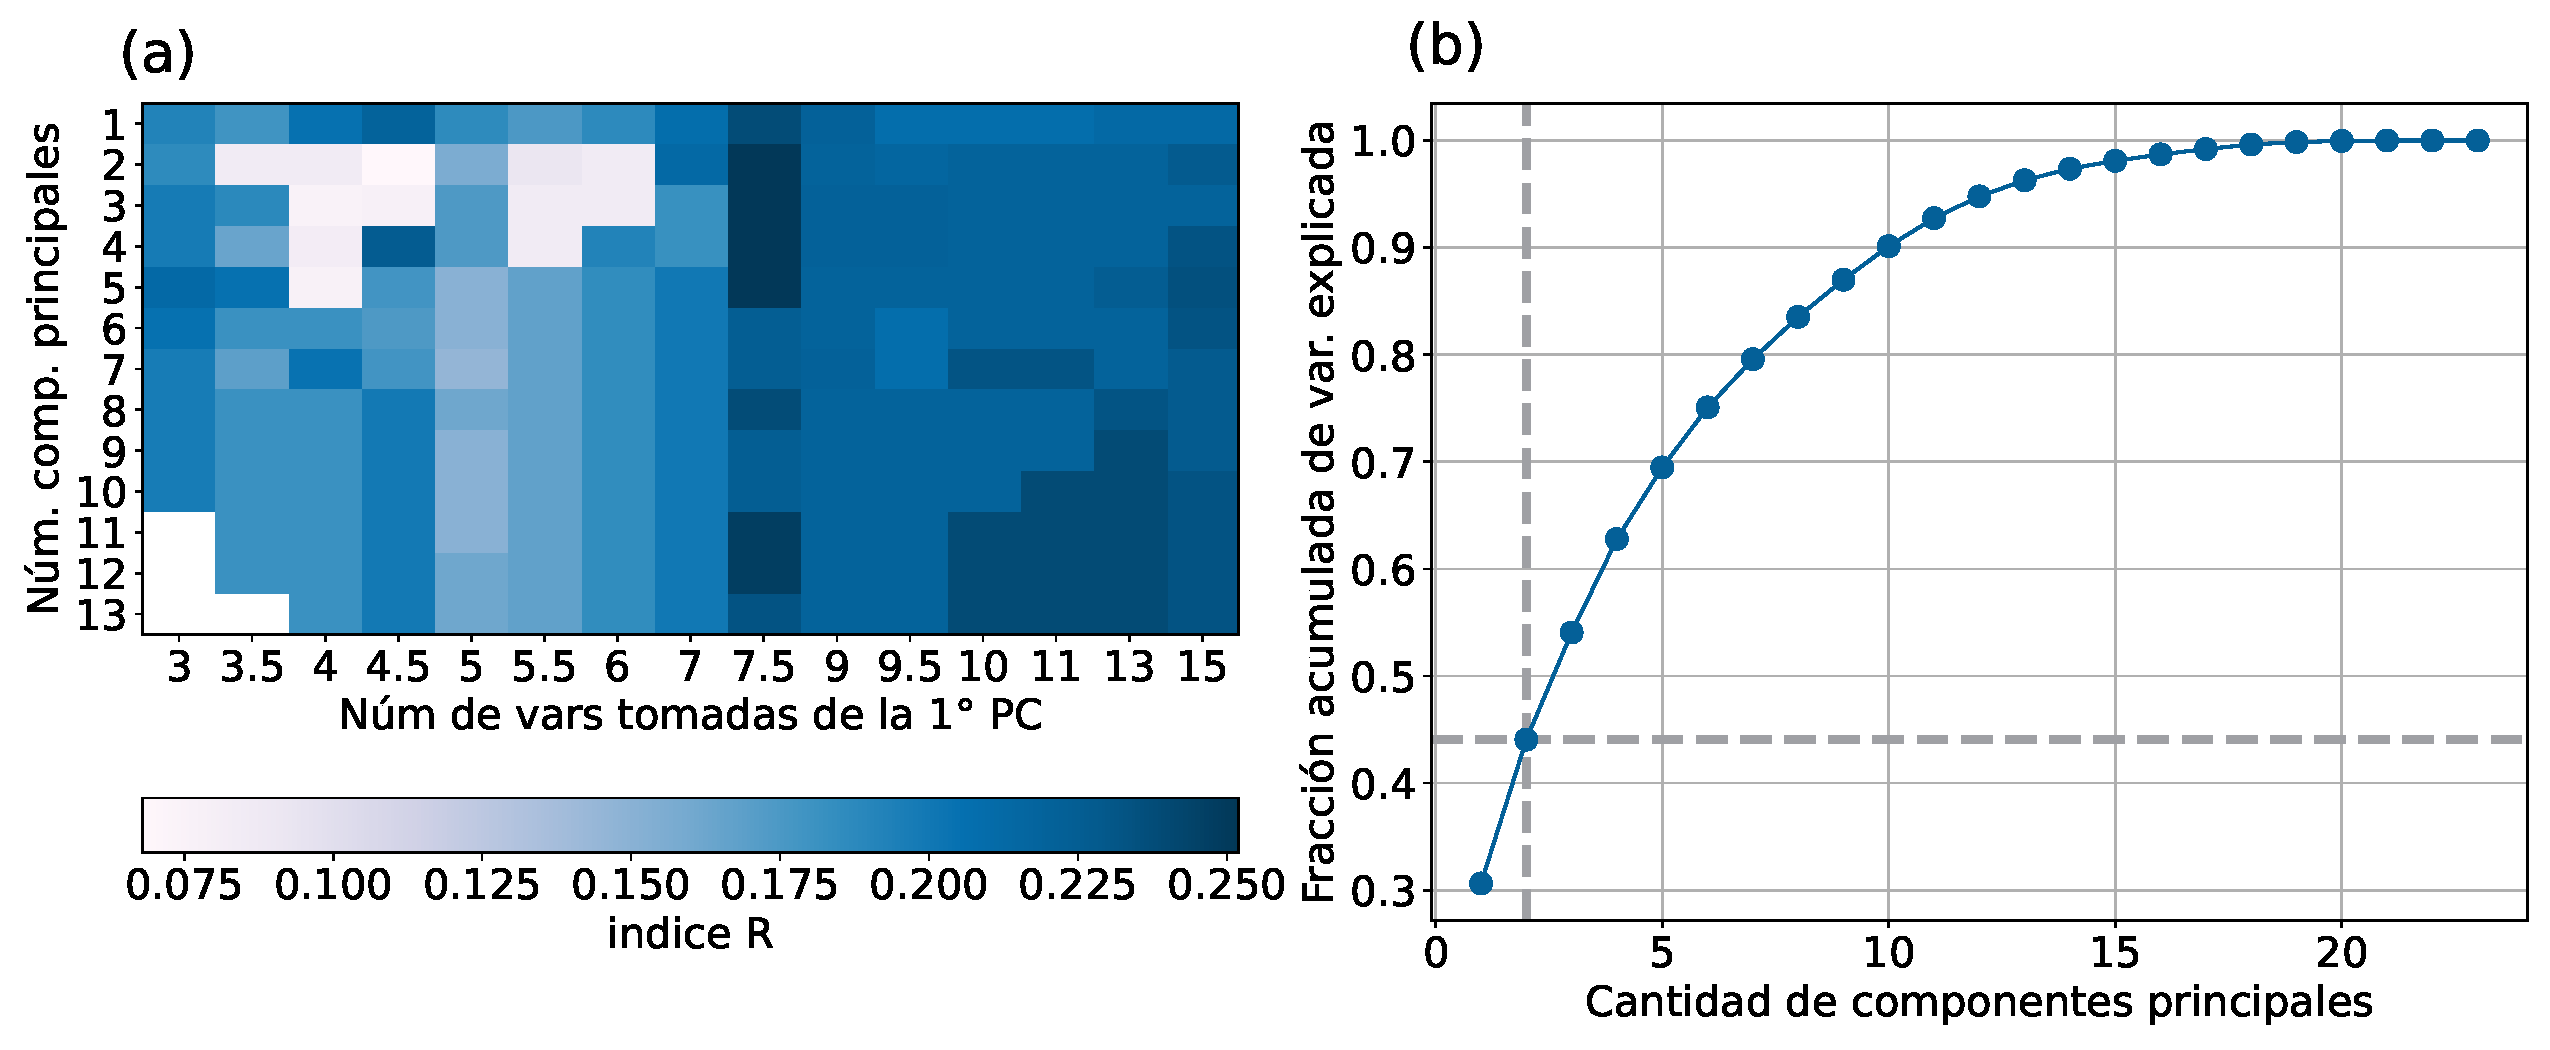
\includegraphics[width = 15cm]{figures/ch03/PCA_clustering/Primer tiempo/eleccionPCs_cfk_pres_ar_control.pdf} 
    \caption{Definición del número de componentes principales y las variables que se utilizarán luego para hacer clustering. En \textbf{(a)} se ve el valor del índice R (validación con las etiquetas externas de los relatos) ante un barrido en el número de PCs y el número de variables tomada en la primer componente principal. Se graficó hasta trece componentes pues el comportamiento de allí en adelante es el mismo. En \textbf{(b)} se ve la fracción acumulada de varianza de los datos solo utilizando las variables que maximizan el índice R. En línea punteada se marca el valor para dos componentes principales.}
\label{fig:cap3_defPCs_cfkArCamp}
\end{figure}


Las primeras dos componentes principales se pueden observar en la Figura \ref{fig:cap3_PC1vsPC2cfkArCamp}. Se puede ver que la primer componente es una combinación lineal donde el mayor peso lo tiene el número de palabras y todas las variables estructurales de redes. La segunda componente es una combinación de todas las variables de sentimiento, donde intensidad tiene un peso menor al resto.


\begin{figure}[h]
    \centering
    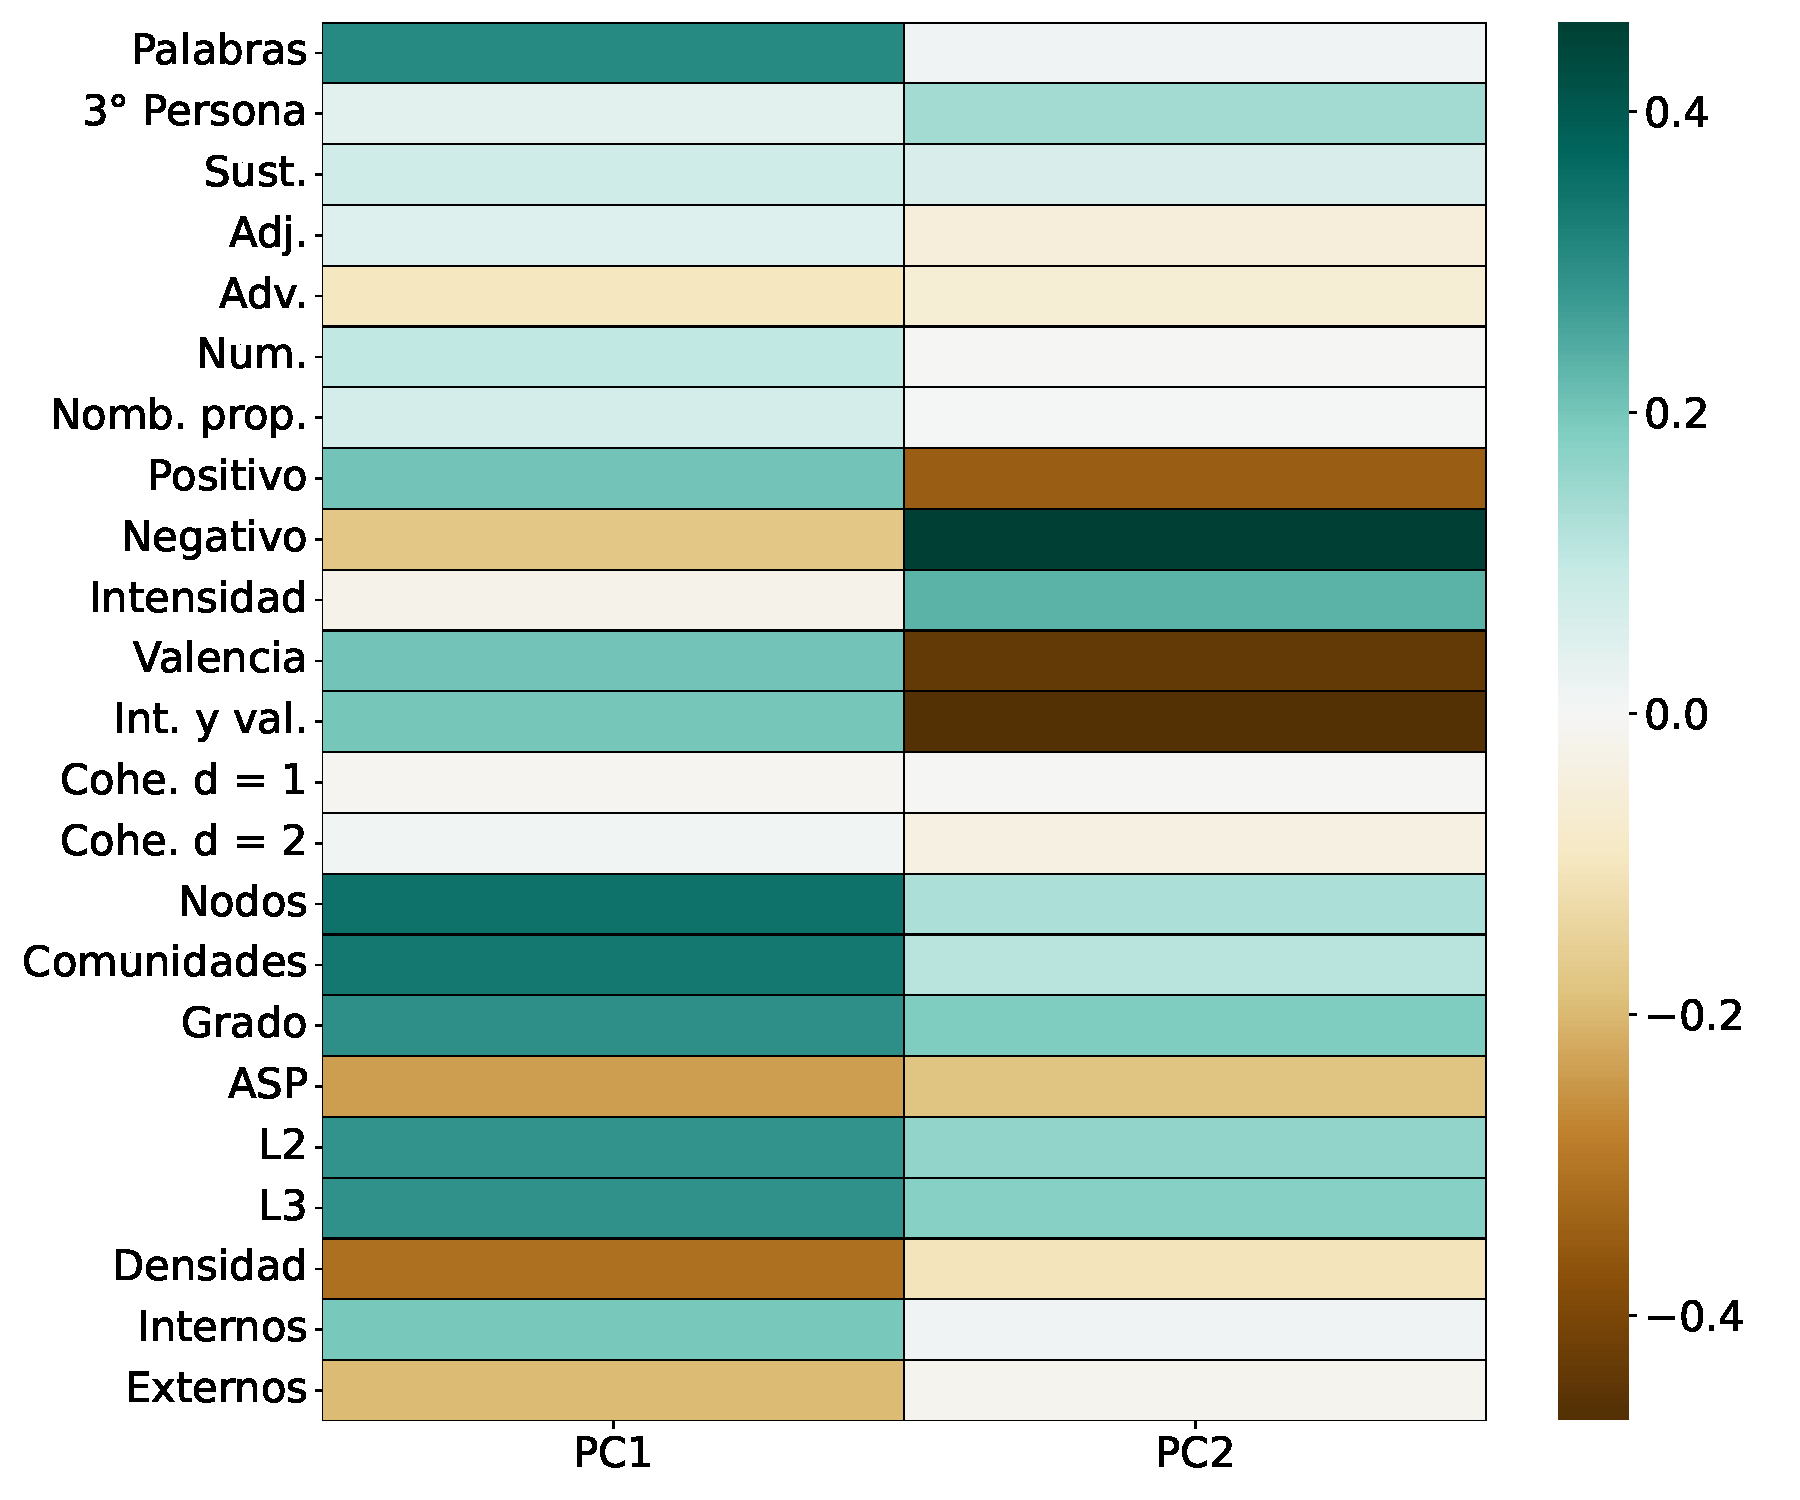
\includegraphics[width = 15cm]{figures/ch03/PCA_clustering/Primer tiempo/2PCs_cfk_pres_ar_control.pdf} 
    \caption{Primeras dos componentes principales que maximizan la validación externa del índice R para los relatos de CFK, Arabia y campeones.}
\label{fig:cap3_2PCscfkArCamp}
\end{figure}

Por último se graficó los relatos proyectados en la primera y segunda componente principal. El color denota las diferentes condiciones, la forma los distintos grupos. El índice R de esta configuración es de 0,25, sube a 0,34 al tratar a Arabia y CFK como una única condición. La matriz de confusión se puede ver en la Tabla \ref{tab:confusion_matrix_CFKARcamp}


\begin{table}[htbp]
    \centering
    \begin{tabular}{|l|c|c|c|c|}
        %\hline
        \cline{2-5}
        \multicolumn{1}{|c|}{} & \multicolumn{4}{c|}{\textbf{Condición real}} \\
        \cline{2-5}
        \multicolumn{1}{|c|}{} & & \textbf{CFK} & \textbf{Arabia} & \textbf{Campeones} \\
        \hline
        \multirow{2}{*}{\textbf{Condición clustering}} & \textbf{CFK y Arabia} & 41 & 35 & 4 \\
        \cline{2-5}
        & \textbf{Campeones} & 12 & 18 & 50 \\
        \hline
    \end{tabular}
    \caption{Matriz de confusión \colorbox{yellow}{le digo asi?} para las condiciones de CFK, Arabia y campeones.}
    \label{tab:confusion_matrix_CFKARcamp}
\end{table}

\begin{figure}[h]
    \centering
    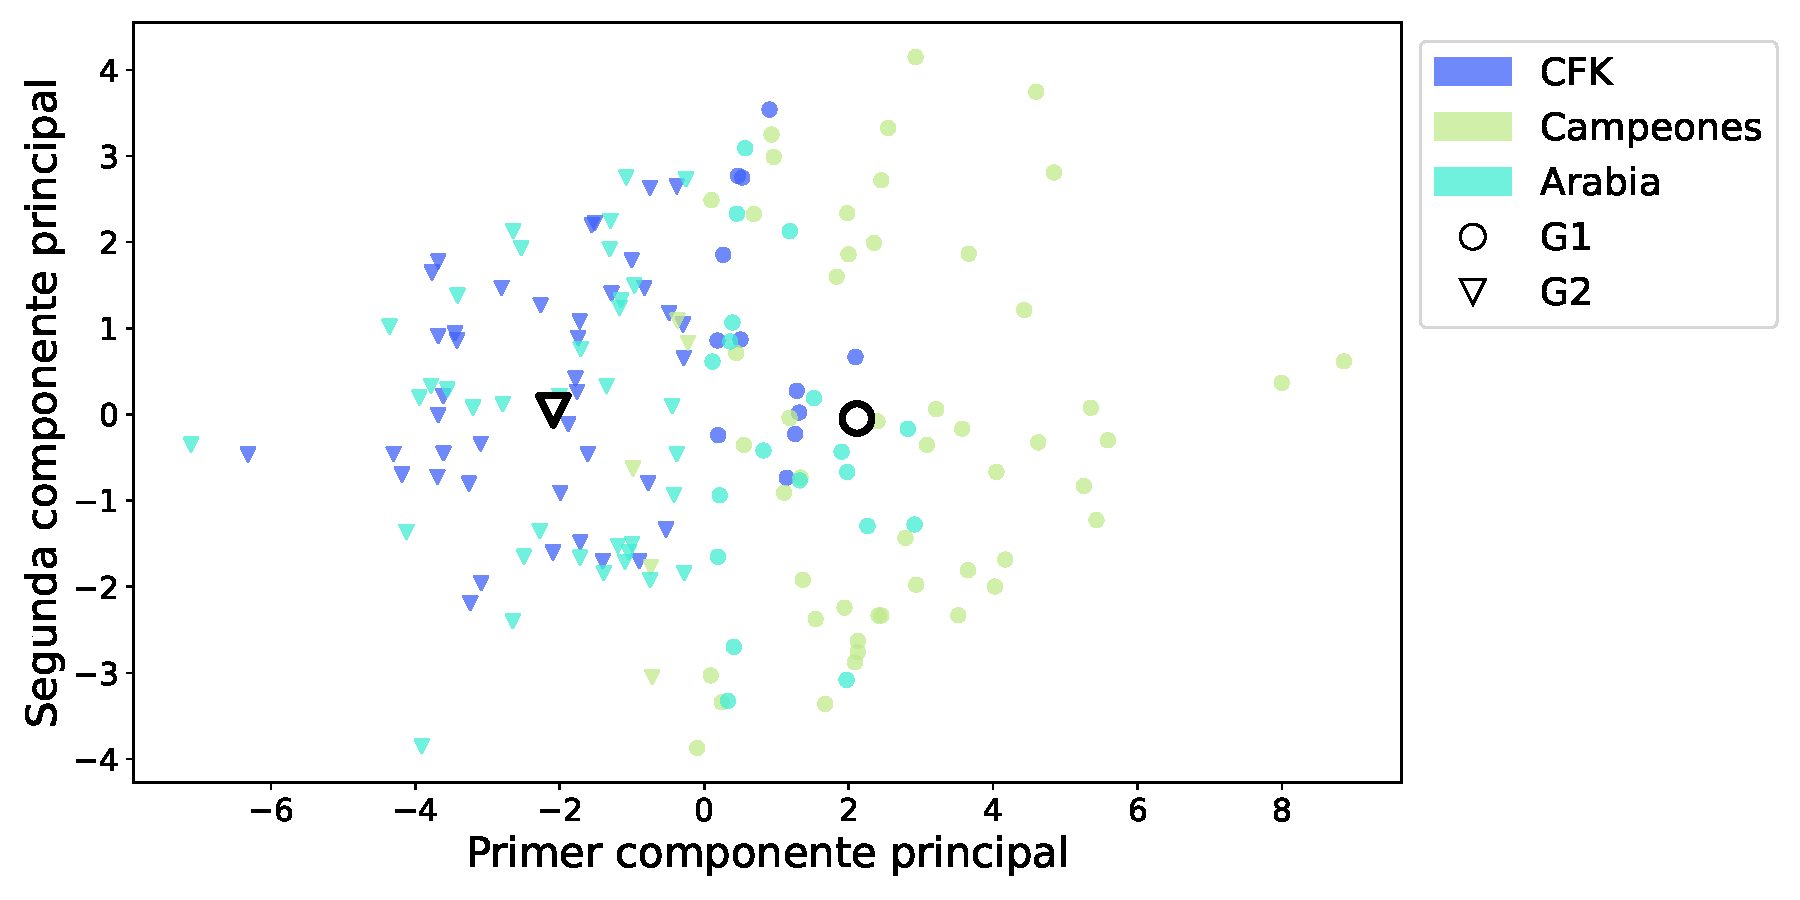
\includegraphics[width = 15cm]{figures/ch03/PCA_clustering/Primer tiempo/cfkArCamp_NOenespaciocosine_PC1vsPC2_markersclusters_colortemas.pdf} 
    \caption{Relatos de CFK, Arabia y campeones proyectados en la primera y segunda componente principal. El color denota las diferentes condiciones y la forma el grupo al que pertenecen. \colorbox{yellow}{CAMBIA C1 C2 POR G1 G2}}
\label{fig:cap3_PC1vsPC2cfkArCamp}
\end{figure}


\section{Agrupamiento natural (o clustering) en la segunda entrevista}

\colorbox{yellow}{la de presencial y control creo q es la idea, los cuantificadores son los que encontramos en la segunda entrevista y fin pero ya la escribo x por las dudas}

En esta sección se contará los resultados del agrupamiento de los datos en la segunda entrevista. Se utilizará las mismas componentes principales que en la primer entrevista. Para las condiciones de presencial y control se utilizaran las 9 componentes principales de la Figura \ref{fig:cap3_9PCscontrolpres} y para las condiciones de CFK, Arabia y campeones las dos componentes de \ref{fig:cap3_2PCscfkArCamp}.

Los resultados para las condiciones de presencial y control se pueden ver en la Figura \ref{fig:cap3_PC1vsPC2pres_control_segundot}, donde se proyectó los relatos en la primera y segunda componente principal y se marcó los grupos con formas y las condiciones con formas. El índice R de la configuración es de 0,13, el mismo bajó respecto de la primer entrevista. La matriz de confusión se puede ver en la Tabla \ref{tab:confusion_matrix_PyC_2t}. Se tiene que el 78$\%$ de los relatos de control fueron bien clasificados y el 62$\%$ de los de presencial.

\begin{figure}[H]
    \centering
    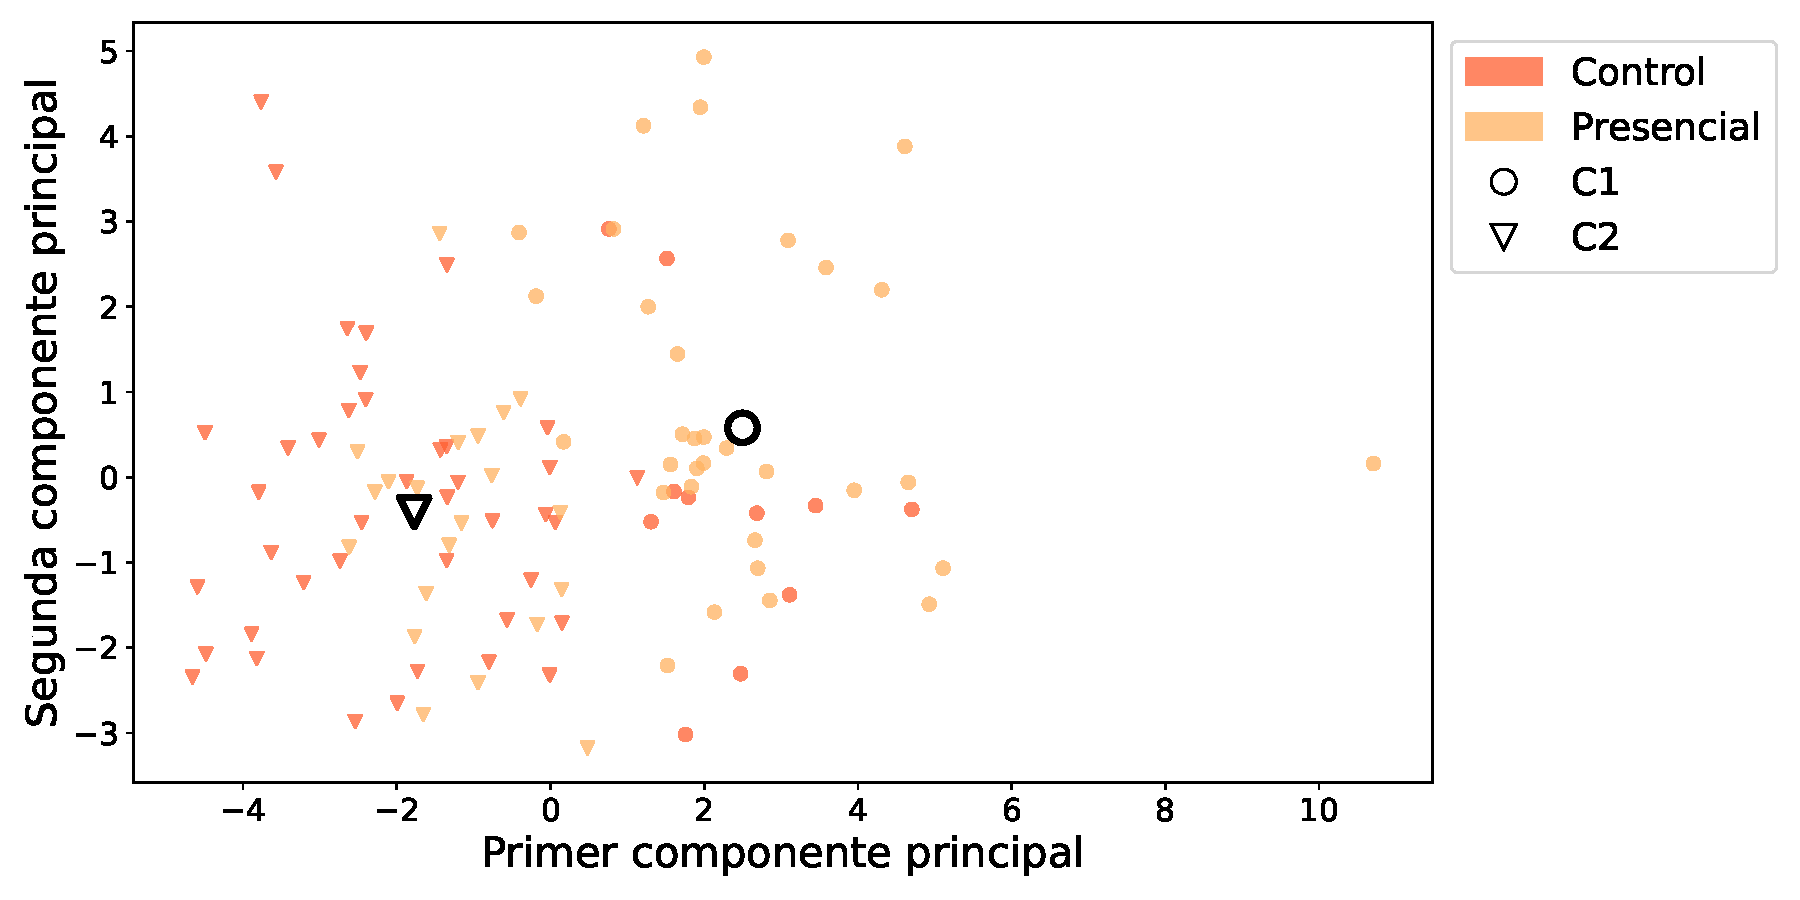
\includegraphics[width = 15cm]{figures/ch03/PCA_clustering/Segundo tiempo/presvscontrol_SEGUNDA_ENT_NOenespaciocosine_PC1vsPC2_markersclusters_colortemas.pdf} 
    \caption{Relatos de las condiciones de presencial y control en la segunda entrevista proyectador en la primera y segunda componente principal y agrupados en dos grupos. Los grupos se denota con las formas, las condiciones con colores.}
\label{fig:cap3_PC1vsPC2pres_control_segundot}
\end{figure}

\begin{table}[htbp]
    \centering
    \begin{tabular}{|l|c|c|c|}
        %\hline
        \cline{3-4}
        \multicolumn{1}{c|}{} & \multicolumn{3}{c|}{\textbf{Condición real}} \\
        \cline{3-4}
        \multicolumn{1}{c}{} & & \textbf{Control} & \textbf{Presencial} \\
        \hline
        \multirow{2}{*}{\textbf{Condición clustering}} & \textbf{Control} & 41 & 20 \\
        \cline{2-4}
        & \textbf{Presencial} & 11 & 32 \\
        \hline
    \end{tabular}
    \caption{Matriz de confusión para las condiciones de presencial y control en la segunda entrevista.}
    \label{tab:confusion_matrix_PyC_2t}
\end{table}


Los resultados para las condiciones de CFK, Arabia y campeones se pueden observar en la Figura \ref{fig:cap3_PC1vsPC2cfkArCamp_segundot}. Allí se puede ver los relatos de las condiciones proyectados en la primer y segunda componente luego de haber hecho el agrupamiento. El índice R del agrupamiento es de 0,25 al igual que en el primer tiempo. Si se toma a CFK y Arabia como una única condición sube a 0,33. La matriz de confusión se puede ver en la Tabla \ref{tab:confusion_matrix_CFKARcamp_2t} donde se puede ver que mas del 90$\%$ de los datos de campeones fueron correctamente clasificádos, el 76$\%$ para CFK y el 73$\%$ para Arabia.

\begin{figure}[H]
    \centering
    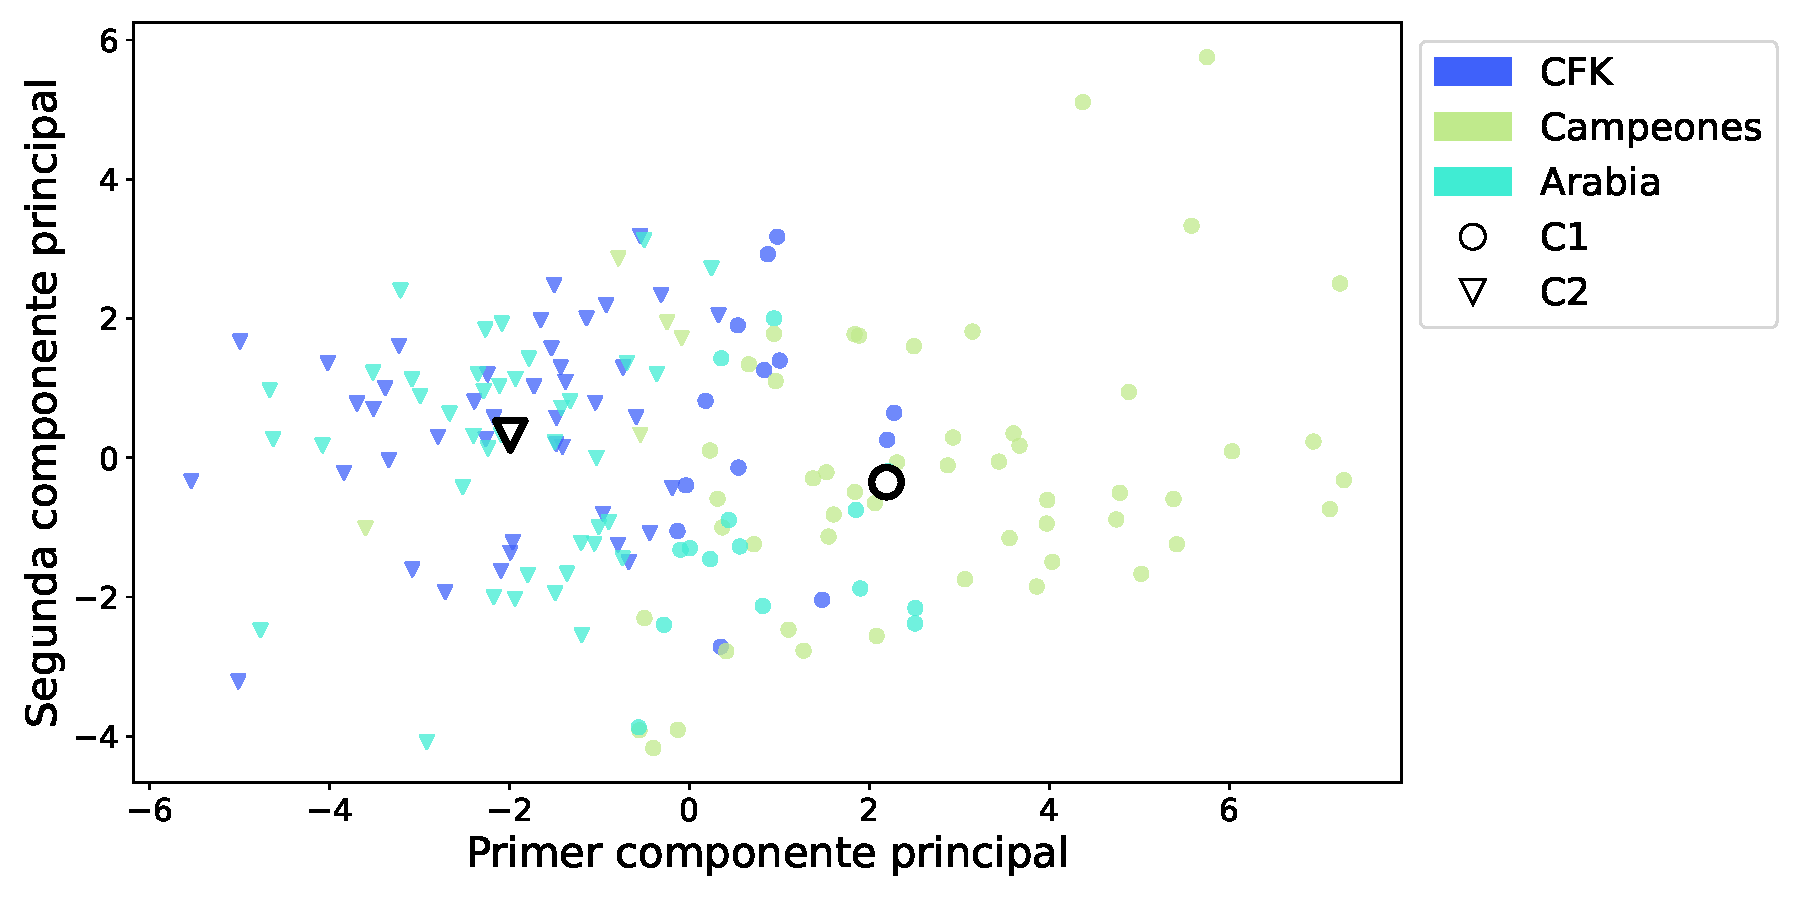
\includegraphics[width = 15cm]{figures/ch03/PCA_clustering/Segundo tiempo/cfkArCamp_SEGUNDA_ENT_NOenespaciocosine_PC1vsPC2_markersclusters_colortemas.pdf} 
    \caption{Relatos de las condiciones de CFK (azul), Arabia (celeste) y campeones (verde) en la segunda entrevista proyectador en la primera y segunda componente principal y agrupados en dos grupos. Los grupos se denota con las formas, las condiciones con colores.}
\label{fig:cap3_PC1vsPC2cfkArCamp_segundot}
\end{figure}

\begin{table}[htbp]
    \centering
    \begin{tabular}{|l|c|c|c|c|}
        %\hline
        \cline{3-5}
        \multicolumn{2}{c|}{} & \multicolumn{3}{c|}{\textbf{Condición real}} \\
        \cline{3-5}
        \multicolumn{1}{c}{} & & \textbf{CFK} & \textbf{Arabia} & \textbf{Campeones} \\
        \hline
        \multirow{2}{*}{\textbf{Condición clustering}} & \textbf{CFK y Arabia} & 42 & 39 & 5 \\
        \cline{2-5}
        & \textbf{Campeones} & 13 & 14 & 50 \\
        \hline
    \end{tabular}
    \caption{"Matriz de confusión" \colorbox{yellow}{le digo asi?} para las condiciones de CFK, Arabia y campeones.}
    \label{tab:confusion_matrix_CFKARcamp_2t}
\end{table}


\section{Comparación entre ambos tiempos}

En esta sección se estudiarán las diferencias de las componentes principales de cada condición por el paso del tiempo. Para ello se realizó un one way ANOVA para cada condición y se observó en cuales componentes las medias tenían diferencias significativas.

Recordando el resultado de la sección \ref{sec:PCAyclustering}.\ref{sec:PCscamparCFK} en la Figura \ref{fig:cap3_2PCscfkArCamp}, la primer componente esta compuesta principalmente por las variables estructurales de redes y el número de palabras, mientras que en la segunda componente tienen mayor peso en la combinación lineal las variables de sentimiento.

Para la condición de Arabia se observó diferencias significativas en las dos componentes principales. En particular para la primer componente se tenía F$_{1,49}$ = 13,05, p = 0,0007 y $\eta_g^2$ = 0,06. En la Figura \ref{fig:cap3_ArPC1} se puede observar la distribución de la primer componente para cada tiempo y también a su derecha se puede ver la media y error estándar de las cuatro variables con mayor peso en la combinación lineal de esta componente. En ella se ve que la primer componente principal disminuye su media en el segundo tiempo. Viendo lo que sucede con las medias de las primeras 4 variables que la componen, se ve que en 3 de ellas la media disminuye. El número de nodos y palabras nos hablan de que el relato en el segundo tiempo en promedio fue mas corto que el primero. \colorbox{yellow}{no se q decir del núm de comunidades y densidad :) un poco lo mismo dicen...}


\begin{figure}[h]
    \centering
    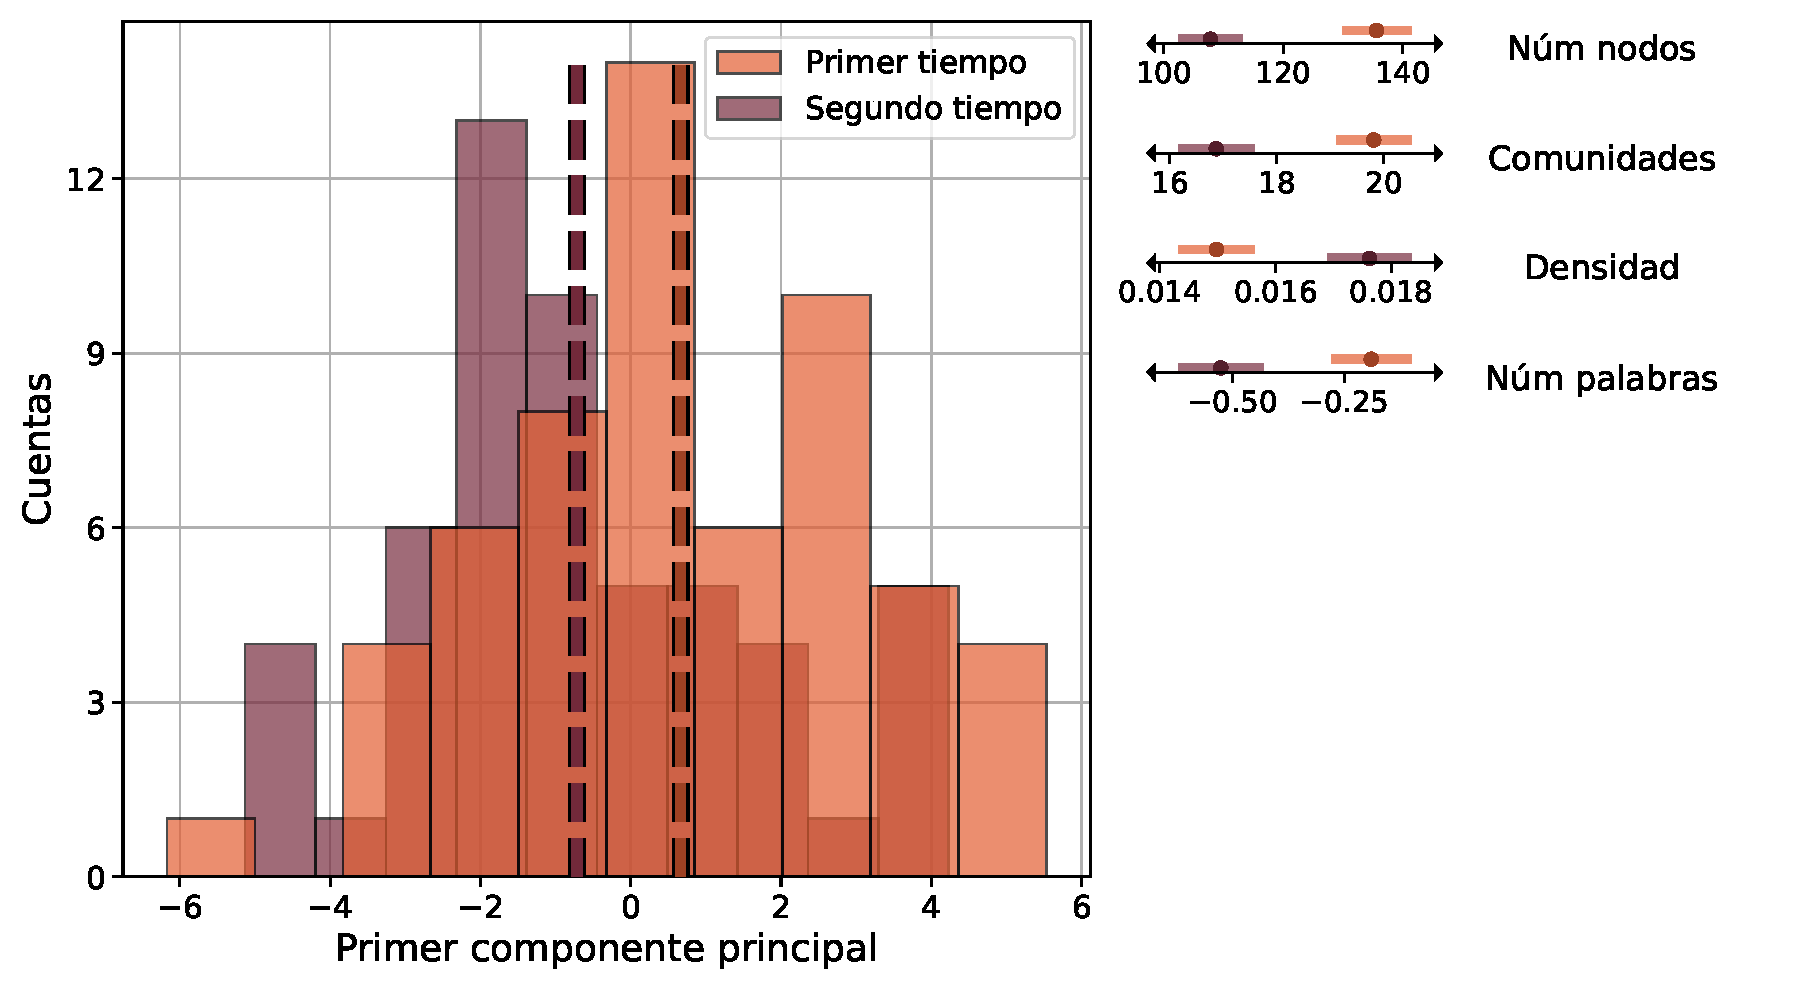
\includegraphics[width = 14cm]{figures/ch03/DosTiempos/arabia_PC1.pdf} 
    \caption{Histogramas de la primer componente principal en el primer y segundo tiempo para la condición de Arabia. En línea punteada se marcan las medias. A la derecha se observan graficadas la media y error estándar de las cuatro variables que mayor peso tienen en la combinación lineal de la primer componente principal.}
\label{fig:cap3_ArPC1}
\end{figure}

Para la segunda componente principal de Arabia se tuvo valores F$_{1,49}$ = 4,13, p = 0,048 y $\eta_g^2$ = 0,04. En la Figura \ref{fig:cap3_ArPC2} se puede observar que la media disminuye en el segundo tiempo. A la derecha se puede ver que las variables que mas pesan en la combinación lineal, que son las de sentimiento no tienen diferencias significativas entre ambos tiempos por separado. 

\begin{figure}[h]
    \centering
    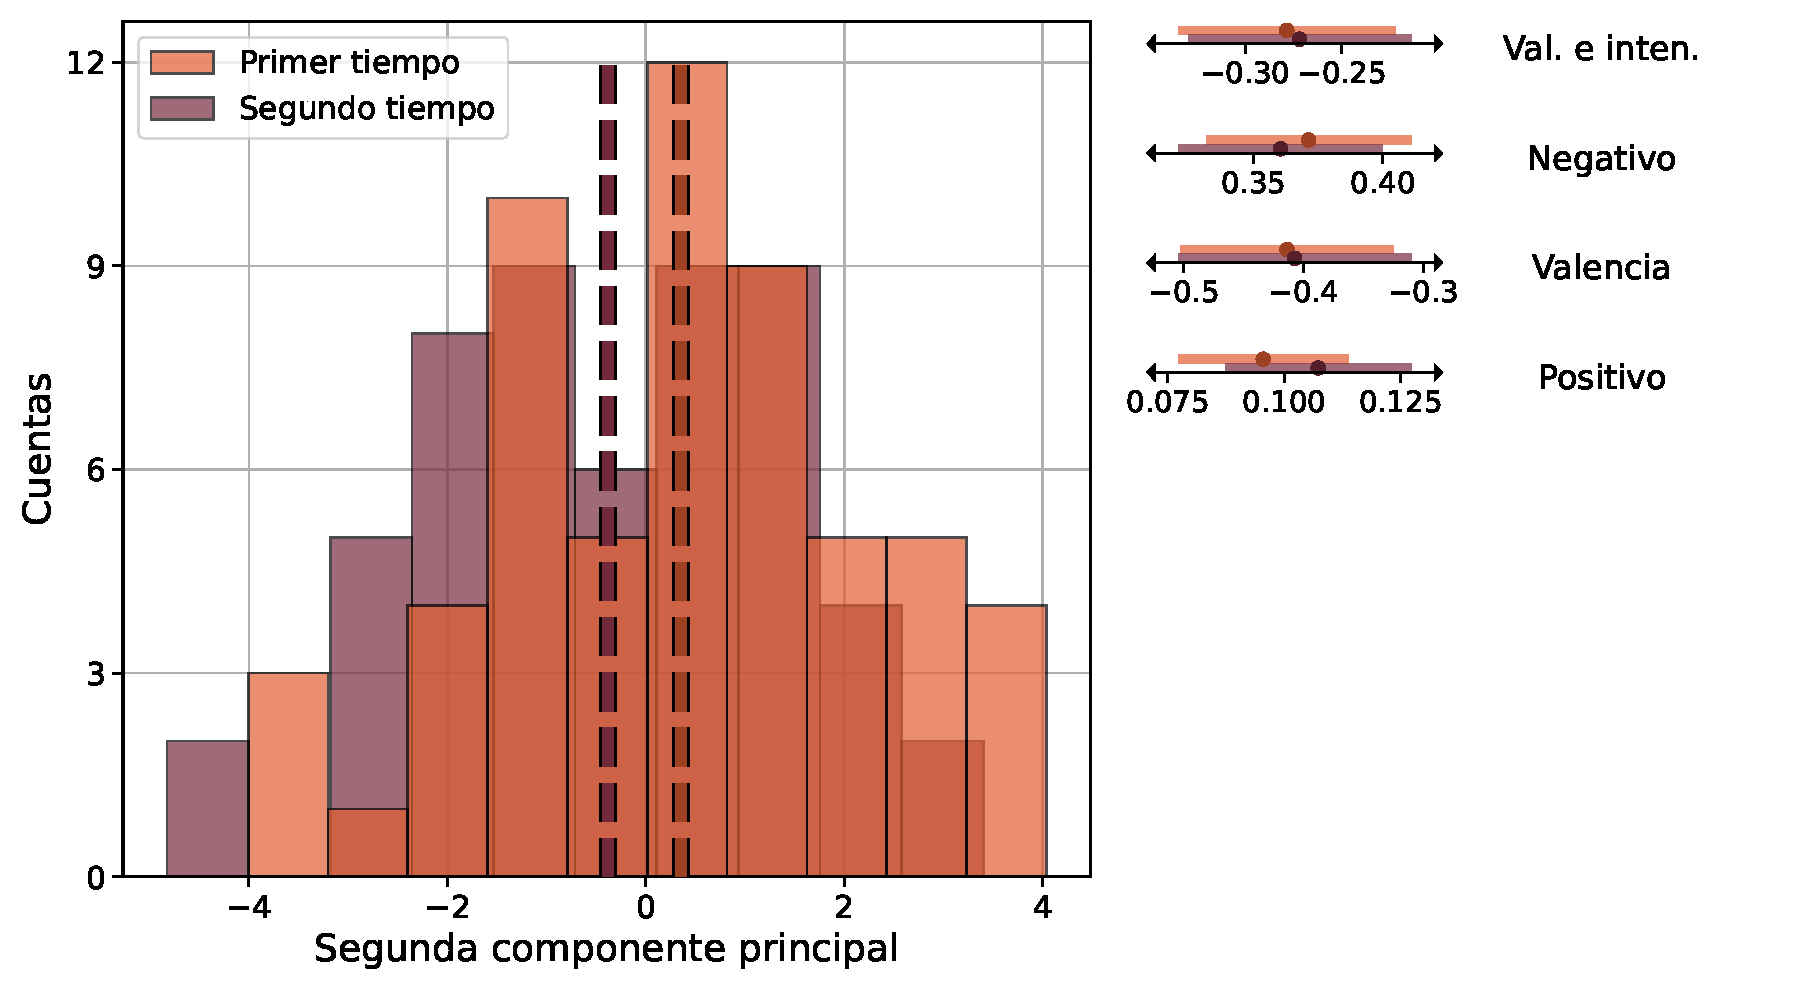
\includegraphics[width = 14cm]{figures/ch03/DosTiempos/arabia_PC2.pdf} 
    \caption{Histogramas de la segunda componente principal en el primer y segundo tiempo para la condición de Arabia. En línea punteada se marcan las medias. A la derecha se observan graficadas la media y error estándar de las cuatro variables que mayor peso tienen en la combinación lineal de la segunda componente principal.}
\label{fig:cap3_ArPC2}
\end{figure}

Para la condición de CFK se observó diferencias significativas solo en la primer componente principal. El valor del F de ANOVA fue de F$_{1,52}$ = 5,83 con p = 0,019 y $\eta_g^2$ = 0,02. En la Figura \ref{fig:cap3_cfkPC1} se observa que la media disminuye en el segundo tiempo aunque \colorbox{yellow}{no se como decir bien que el eta y p nos dicen que es menos significativo que arabia}. En tanto a las variables mas importantes en la combinación lineal, se ve un comportamiento similar al de Arabia, pero en este caso el número de palabras no tiene diferencias significativas entre ambos tiempos, pero sí la tiene el número de nodos. \colorbox{yellow}{no se bien q decir}


\begin{figure}[h]
    \centering
    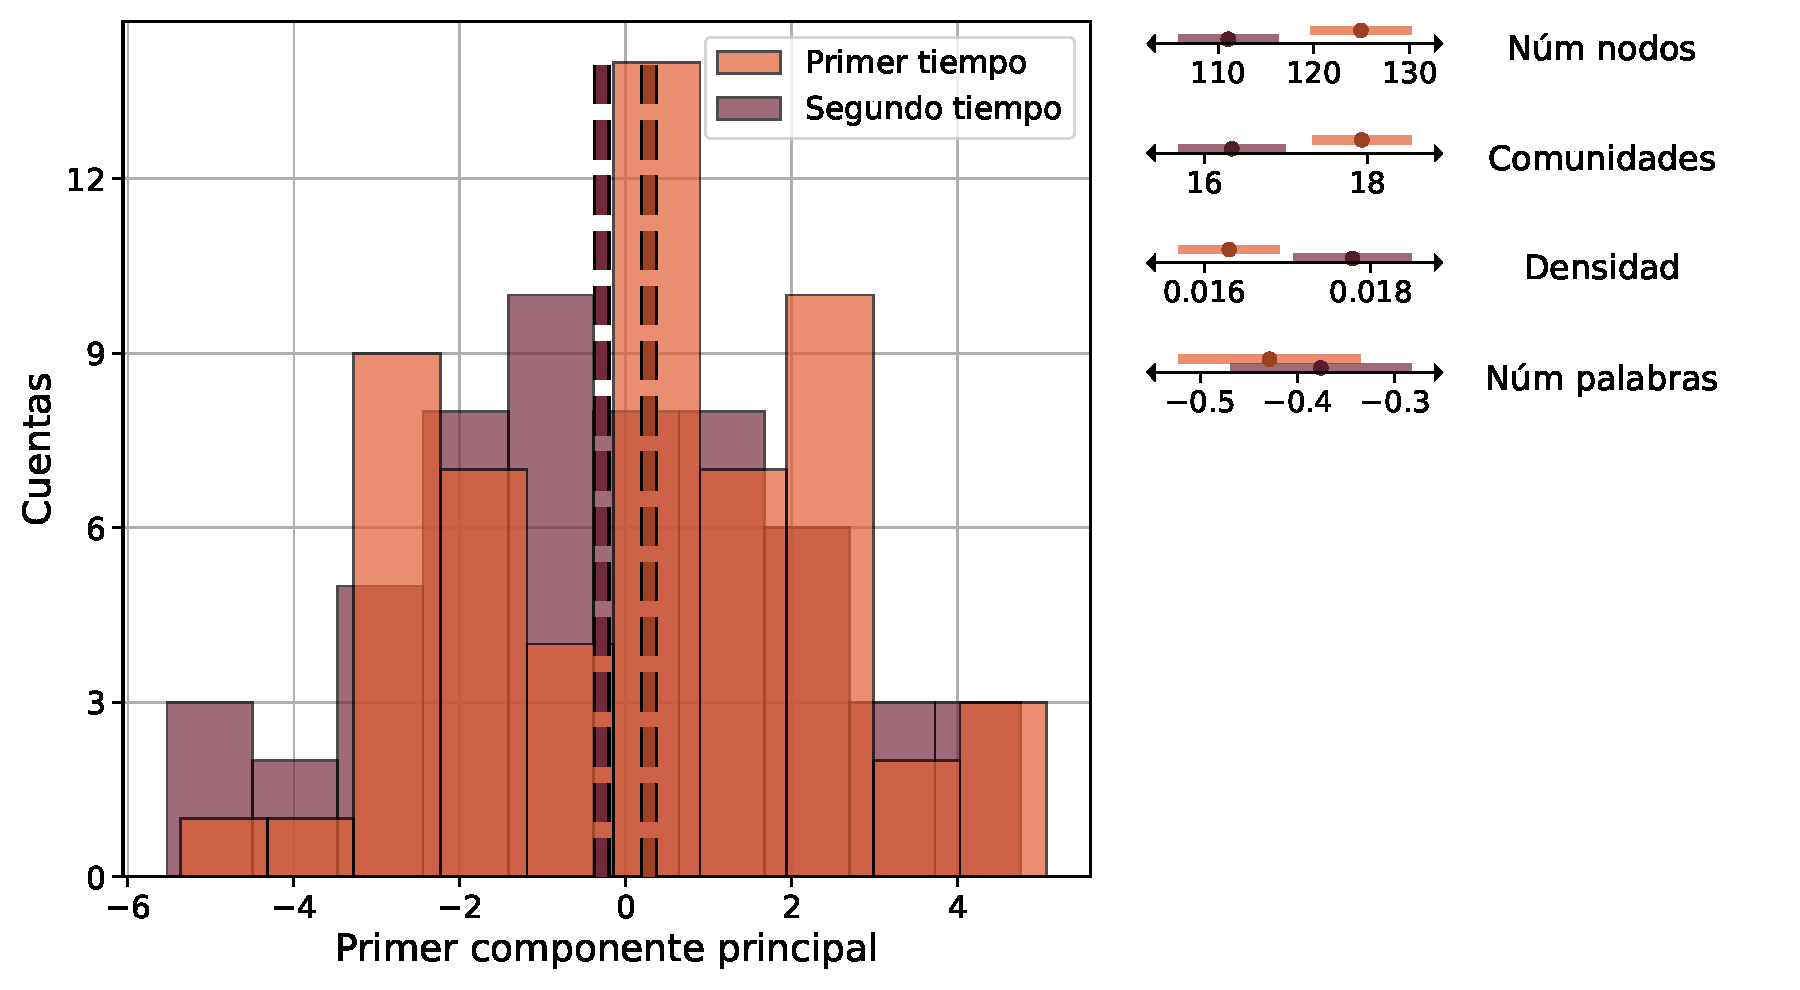
\includegraphics[width = 14cm]{figures/ch03/DosTiempos/cfk_PC1.pdf} 
    \caption{Histogramas de la primer componente principal en el primer y segundo tiempo para la condición de CFK. En línea punteada se marcan las medias. A la derecha se observan graficadas la media y error estándar de las cuatro variables que mayor peso tienen en la combinación lineal de la primer componente principal.}
\label{fig:cap3_cfkPC1}
\end{figure}

Para la condición de presencial solo se tuvo diferencias significativas en la media de la segunda componente principal con F$_{1,47}$ = 5,86, p = 0,019 y $\eta_g^2$ = 0,04. Los resultados se pueden observar en la Figura \ref{fig:cap3_presPC2}. Nuevamente la media disminuye en el segundo tiempo. En este caso a diferencia de Arabia si se observa diferencia significativa entre las medias de las variables mas importantes de la componente principal. En particular se tiene que el relato en el segundo tiempo tiende a una valencia mas neutra, baja la negatividad y sube la positividad. \colorbox{yellow}{creo q nada mas no?}

\begin{figure}[h]
    \centering
    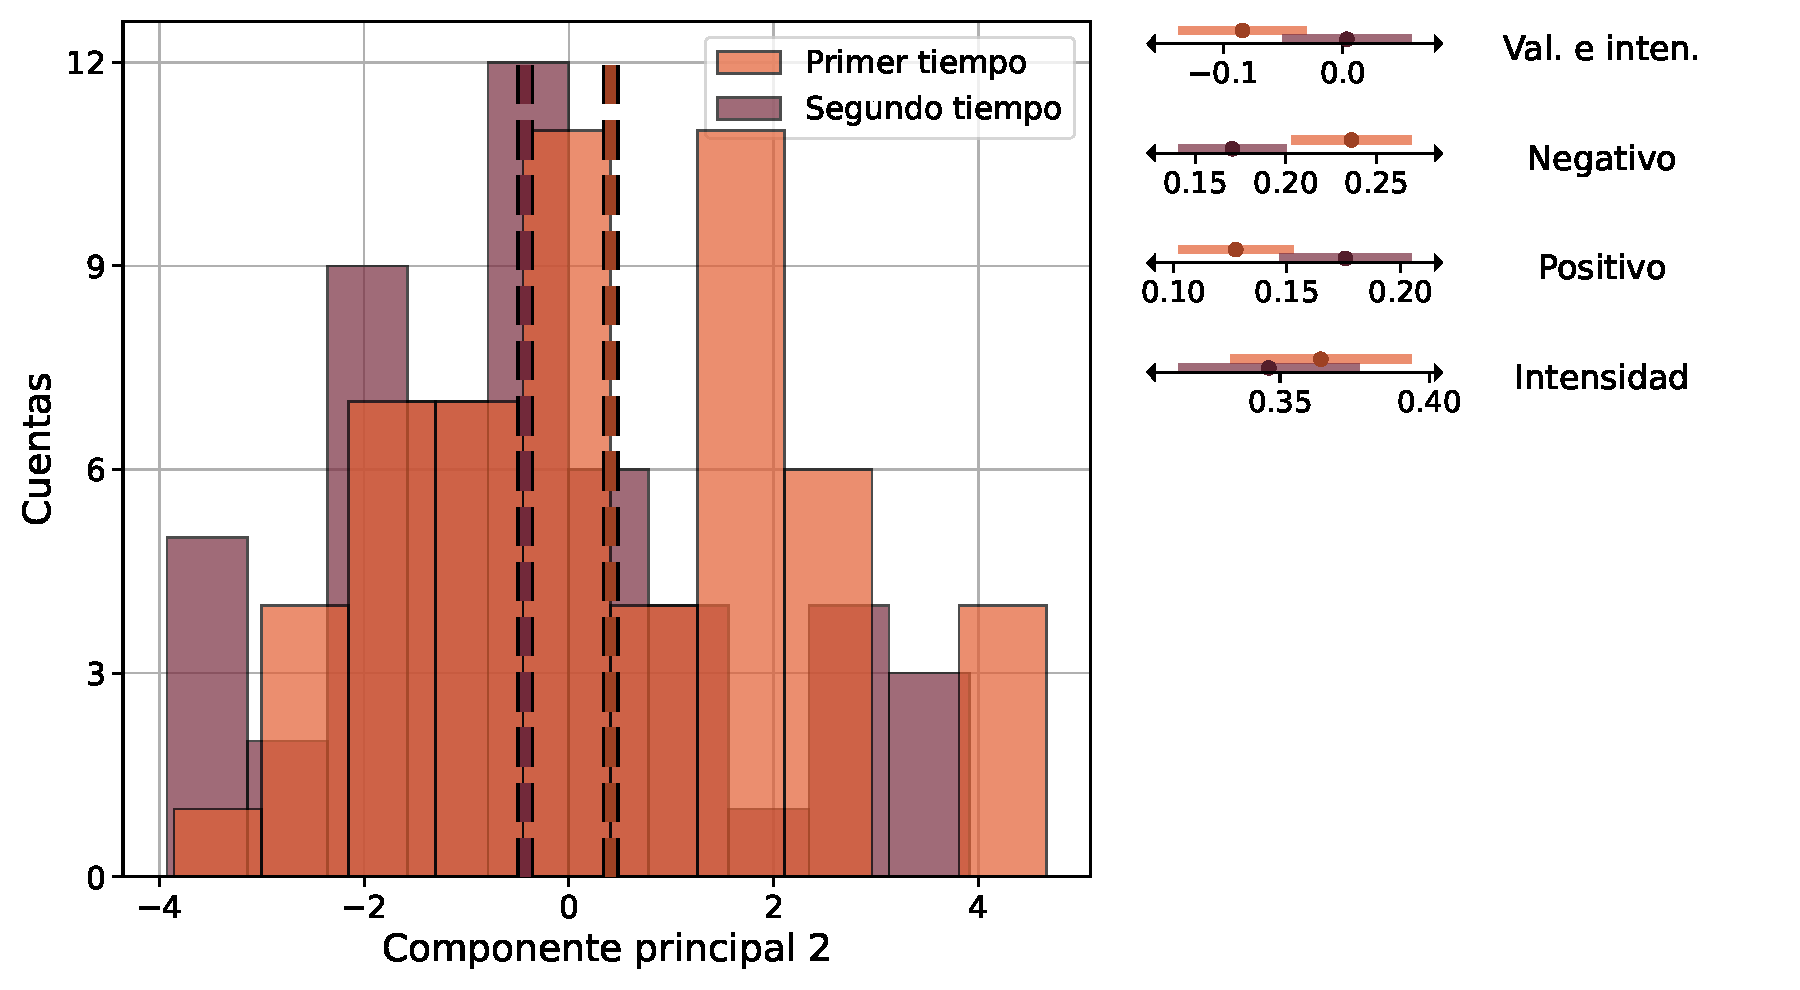
\includegraphics[width = 14cm]{figures/ch03/DosTiempos/presencial_PC2.pdf} 
    \caption{Histogramas de la segunda componente principal en el primer y segundo tiempo para la condición de presencial. En línea punteada se marcan las medias. A la derecha se observan graficadas la media y error estándar de las cuatro variables que mayor peso tienen en la combinación lineal de la segunda componente principal.}
\label{fig:cap3_presPC2}
\end{figure}

Finalmente para la condición de campeones, el relato mas intenso (\colorbox{yellow}{no se si poner eso aca, pero en discusión si discutir el hecho de que el relato mas intenso es el q no tiene diferencias)} no tiene ninguna componente principal con diferencias significativas.



%-------------------------------------------------------
%\chapter{Discusión}
%\label{ch:ch4}
%\input{sections/ch4.tex}


%-------------------------------------------------------
%\chapter{Conclusiones y perspectivas}
%\label{ch:ch5}
%\\input{sections/conclusion.tex}

%--------------------------------------------------------


%--------------------------------------------------------
%\bibliographystyle{IEEEtran}
%\bibliography{IEEEabrv,cite.bib}{}

%__________________________________________________________
%apendices
%\chapter{Apéndices}
%\begin{apendice}\label{ap:conestelabellocitas}

Selección de eventos

tengo que contar de dónde saque los temas, los participantes (edad genero y eso) y el gráfico de valencia vs intensidad, VA ese gráfico por ahi va en materiales y métodos y la discusión de por qué se eligieron esos (queríamos diferente valencia e intensidad), y bueno, también hay que contar del filler

\end{apendice}

\begin{apendice}\label{ap:otrolabelacitar}
y aca va lo que queres poner en el apéndice
 
\end{apendice}

% %--------------------------------------------------------
% % 'Publication 1'
% \chapter*{Publications}
% \chapter*{Publication 1}
% \addtocontents{toc}{\protect{\addvspace{3.0ex plus 1pt}}}
% \addcontentsline{toc}{chapter}{\protect{Publication 1}}
% \input{sections/paper1.tex}
% \includepdf[pages={-}]{papers/paper1.pdf}
% %
% %--------------------------------------------------------
% % 'Publication 2'
% \chapter*{Publication 2}
% \addtocontents{toc}{\protect{\addvspace{3.0ex plus 1pt}}}
% \addcontentsline{toc}{chapter}{\protect{Publication 2}}
% \input{sections/paper2.tex}
% \includepdf[pages={-}]{papers/paper2.pdf}

\end{document}
